\title{Monografia - Janderson}

\documentclass[
	% -- opções da classe memoir --
	12pt,				% tamanho da fonte
    oneside,			% Tipo de impressão, frente-verso(twoside) ou apenas frente(oneside)
	a4paper,			% tamanho do papel. 
	% -- opções da classe abntex2 --
	chapter=TITLE,		% títulos de capítulos convertidos em letras maiúsculas
	% -- opções do pacote babel --    
	english,			% idioma adicional para hifenização
	brazil				% o último idioma é o principal do documento    
	]{abntex2}
    
    %\renewcommand{\ABNTEXpartfontsize}{\normalsize}
	%\renewcommand{\ABNTEXchapterfontsize}{ \large}
	%\renewcommand{\ABNTEXsectionfontsize}{\normalsize}
	%\renewcommand{\ABNTEXsubsectionfontsize}{\normalsize}

% ---
% Pacotes básicos 
% ---
\usepackage{lmodern}			% Usa a fonte Latin Modern			
\usepackage[T1]{fontenc}		% Selecao de codigos de fonte.
\usepackage[utf8]{inputenc}		% Codificacao do documento (conversão automática dos acentos)
\usepackage{lastpage}			% Usado pela Ficha catalográfica
\usepackage{indentfirst}		% Indenta o primeiro parágrafo de cada seção.
\usepackage{color}				% Controle das cores
\usepackage{graphicx}			% Inclusão de gráficos
\usepackage{microtype} 			% para melhorias de justificação
\usepackage{todonotes}
\usepackage{tabularx}


\definecolor{algColor}{RGB}{255,206,206} % rgb(255, 206, 206)

% Pacotes para algoritmos/pseudo-código
\usepackage{listings}

\renewcommand{\lstlistingname}{Programa}

\lstset
{ %Formatting for code in appendix
    language=C,
    basicstyle=\footnotesize,
    numbers=left,
    stepnumber=1,
    frame = single,
    showstringspaces=false,
    tabsize=2,
    breaklines=true,
    xleftmargin=10pt,
    breakatwhitespace=false,
    extendedchars=true,
    literate={á}{{\'a}}1 
             {ã}{{\~a}}1
             {é}{{\'e}}1
             {í}{{\'i}}1
             {õ}{{\~o}}1
             {ç}{{\c{c}}}1,
}

\renewcommand{\lstlistlistingname}{Lista de códigos}

% Configura a ``Lista de Códigos'' conforme as regras da ABNT (para abnTeX2)
\begingroup\makeatletter
\let\newcounter\@gobble\let\setcounter\@gobbletwo
  \globaldefs\@ne \let\c@loldepth\@ne
  \newlistof{listings}{lol}{\lstlistlistingname}
  \newlistentry{lstlisting}{lol}{0}
\endgroup

\renewcommand{\cftlstlistingaftersnum}{\hfill--\hfill}

\let\oldlstlistoflistings\lstlistoflistings
\renewcommand{\lstlistoflistings}{%
   \begingroup%
   \let\oldnumberline\numberline%
   \renewcommand{\numberline}{\lstlistingname\space\oldnumberline}%
   \oldlstlistoflistings%
   \endgroup}
% ---
% Pacotes adicionais, usados apenas no âmbito do Modelo Canônico do abnteX2
% ---
\usepackage{lipsum}				% para geração de dummy text
% ---


% ---
% Pacotes de citações
% ---
%\usepackage[brazilian,hyperpageref]{backref}	 % Paginas com as citações na bibl
\usepackage[alf, abnt-etal-cite=2]{abntex2cite}	% Citações padrão ABNT

% --- 
% CONFIGURAÇÕES DE PACOTES
% --- 

\usepackage{abntex_ufrr_dcc}


% PACOTES DE ALGORITMO

\usepackage{algpseudocode,algorithm}
% Declaracoes em Português

\algrenewcommand\algorithmicend{\textbf{FIM}}
\algrenewcommand\algorithmicdo{\textbf{FAÇA}}
\algrenewcommand\algorithmicwhile{\textbf{ENQUANTO}}
\algrenewcommand\algorithmicfor{\textbf{PARA}}
\algrenewcommand\algorithmicforall{\textbf{PARA TODO}}
\algrenewcommand\algorithmicif{\textbf{SE}}
\algrenewcommand\algorithmicthen{\textbf{ENTÃO}}
\algrenewcommand\algorithmicelse{\textbf{SENÃO}}
\algrenewcommand\algorithmicreturn{\textbf{RETORNE}}
\algrenewcommand\algorithmicfunction{\textbf{FUNÇÃO}}
% New definitions
\algnewcommand\algorithmicswitch{\textbf{ESCOLHA}}
\algnewcommand\algorithmiccase{\textbf{CASO}}
\algnewcommand\algorithmicassert{\texttt{assert}}
\algnewcommand\Assert[1]{\State \algorithmicassert(#1)}%
% New "environments"
\algdef{SE}[SWITCH]{Switch}{EndSwitch}[1]{\algorithmicswitch\ #1\ \algorithmicdo}{\algorithmicend\ \algorithmicswitch}%
\algdef{SE}[CASE]{Case}{EndCase}[1]{\algorithmiccase\ #1}{\algorithmicend\ \algorithmiccase}%
\algtext*{EndSwitch}%
\algtext*{EndCase}%


% Rearranja os finais de cada estrutura
\algrenewtext{EndWhile}{\algorithmicend\ \algorithmicwhile}
\algrenewtext{EndFor}{\algorithmicend\ \algorithmicfor}
\algrenewtext{EndIf}{\algorithmicend\ \algorithmicif}
\algrenewtext{EndFunction}{\algorithmicend\ \algorithmicfunction}

% O comando For, a seguir, retorna 'para #1 -- #2 até #3 faça'
\algnewcommand\algorithmicto{\textbf{até}}
\algrenewtext{For}[3]%
{\algorithmicfor\ #1 $\gets$ #2 \algorithmicto\ #3 \algorithmicdo}


% ---
% Configurações do pacote backref
% Usado sem a opção hyperpageref de backref
%\renewcommand{\backrefpagesname}{Citado na(s) página(s):~}
% Texto padrão antes do número das páginas
%\renewcommand{\backref}{}
% Define os textos da citação
%\renewcommand*{\backrefalt}[4]{
%	\ifcase #1 %
%		Nenhuma citação no texto.%
%	\or
%		Citado na página #2.%
%	\else
%		Citado #1 vezes nas páginas #2.%
%	\fi}%
% ---

% ---
% Informações de dados para CAPA e FOLHA DE ROSTO
% ---
\titulo{\large{Aplicação de Técnicas de Data Mining para Avaliar e classificar os Dados Socioeconômicos dos Candidatos do Vestibular da UFRR de 2017}}

\autor{JANDERSON ALMEIDA DOS SANTOS}
\local{Boa Vista - RR}
\data{2019}
\orientador{Delfa Mercedes Huatuco Zuasnabar}

\tipotrabalho{Monografia}

\preambulo{Monografia de Graduação apresentada ao Departamento de Ciência da Computação da Universidade Federal de Roraima como requisito parcial para a obtenção do grau de Bacharel em Ciência da Computação.}

%Trabalho de conclusão de curso  na área de Verificação de Software desenvolvido na UFRR com o %objetivo \textcolor{red}{VERIFICAR O PADRÃO DOS OUTROS TCC} de gerar casos de teste para %sistemas embarcados críticos	

% ---

%-- Informações de dado para a FOLHA DE APROVAÇÃO
\renewcommand{\dataDefesa}{10 de Julho de 2019}
\renewcommand{\orientadorBanca}{Prof. MSc.Delfa Mercedes Huatuco Zuasnabar}
\renewcommand{\primeiroMembroBanca}{Prof. MSc. Miguel Raymundo Flores Santibañez}
\renewcommand{\segundoMembroBanca}{Prof. MSc. Acauan Cardoso Ribeiro}

% ---
% Configurações de aparência do PDF final

% alterando o aspecto da cor azul
\definecolor{blue}{RGB}{41,5,195}

% informações do PDF
\makeatletter
\hypersetup{
     	%pagebackref=true,
		pdftitle={\@title}, 
		pdfauthor={\@author},
    	pdfsubject={\imprimirpreambulo},
	    pdfcreator={LaTeX with abnTeX2},
		pdfkeywords={abnt}{latex}{abntex}{abntex2}{trabalho acadêmico}, 
		colorlinks=true,       		% false: boxed links; true: colored links
    	linkcolor=blue,          	% color of internal links
    	citecolor=blue,        		% color of links to bibliography
    	filecolor=magenta,      	% color of file links
		urlcolor=blue,
		bookmarksdepth=4
}
\makeatother
% --- 

% --- 
% Espaçamentos entre linhas e parágrafos 
% --- 

% O tamanho do parágrafo é dado por:
\setlength{\parindent}{1.3cm}

% Controle do espaçamento entre um parágrafo e outro:
\setlength{\parskip}{0.2cm}  % tente também \onelineskip

% ---
% compila o indice
% ---
\makeindex
% ---

% ----
% Início do documento
% ----
\begin{document}

% Retira espaço extra obsoleto entre as frases.
\frenchspacing 

% ----------------------------------------------------------
% ELEMENTOS PRÉ-TEXTUAIS
% ----------------------------------------------------------
% \pretextual

% ---
% Capa
% ---
\imprimircapa
% ---

% ---
% Folha de rosto
% (o * indica que haverá a ficha bibliográfica)
% ---
\imprimirfolhaderosto
% ---

% ---
% Inserir folha de aprovação
% ---
\imprimirfolhadeaprovacao
% ---
% Dedicatória
% ---
\begin{dedicatoria}
   \vspace*{\fill}
   \centering
   \noindent
   \textit{Este trabalho é dedicado especialmente para a minha família, que sempre me apoiou nos momentos mais difíceis dessa vida.} \vspace*{\fill}
\end{dedicatoria}
% ---

% ---
% Agradecimentos
% ---
\begin{agradecimentos}
Agradeço, em primeiro lugar, a Deus, meu pai e minha mãe, por estarem sempre comigo, me apoiando nessa longa caminhada que enfrentamos na vida, também, pela compreensão e investimento durante toda a minha vida acadêmica, ao meu irmão e irmã que sempre me apoiaram e que deram sua atenção para me escutar sempre e agradeço também a toda a minha família.
\par
A minha orientadora, professora Delfa, por aceitar a me ajudar na execução deste trabalho, e junto com o coorientador professor Miguel me daram todo o suporte e auxílio. Agradeço aos demais professores da computação que participaram da minha formação, em especial ao professor Herbert Rocha, pela paciência que sempre teve em tirar as minhas dúvidas e pela amizade, os professores Felipe Lobo e Filipe Dwan pelos conselhos que me deram durante o meu curso e ao professor Acauan Cardoso, por todo atenção e disponibilidade que teve em me ajudar no início do meu projeto, onde me deu rumo para que eu concluísse este trabalho.
\par
Agradeço aos amigos do laboratório da NOKIA e Maloca Digital pelo convivio e amizade, especialmente ao Miller Raycell que teve a paciência de ficar lendo o meu projeto a cada parte que eu concluía e na ajuda da tradução do resumo deste trabalho, agradeço também ao meu amigo Luarkian Kaype por sempre tirar as minhas dúvidas no decorrer deste curso. E por fim, agradeço aos demais amigos que conheci no curso e que contribuíram e participaram da minha vida acadêmica de alguma forma: Paulo Victor, Arthur Melo, Anny Walker, Rafael de Sá e entre muitos outros.




\end{agradecimentos}
% ---

% ---
% Epígrafe
% ---
\begin{epigrafe}
    \vspace*{\fill}
	\begin{flushright}
		\textit{Quando as pessoas se machucam, elas aprendem a odiar… quando as pessoas machucam as outras, eles viram odiados e atormentados com a culpa. Mas saiba que a dor permite às pessoas a serem bondosas. A dor permite que todo mundo cresça... e como você cresce é sua responsabilidade. (Masashi Kishimoto)}
	\end{flushright}
\end{epigrafe}
% ---

% ---
% RESUMOS
% ---

% resumo em português
\setlength{\absparsep}{18pt} % ajusta o espaçamento dos parágrafos do resumo
\begin{resumo}
    A mineração de dados tem se tornado uma área crescente durante os últimos anos, devido ao grande crescimento da quantidade de dados que é gerado e a necessidade do mercado por técnicas que sejam eficazes de reconhecer e extrair o conhecimento destes grandes repositórios de dados de forma automatizada. Como não existia na época, um modelo formalizado para o processo de extração de conhecimento a partir de grandes bases de dados o \textit{Knowledge Discovery in Database} (KDD) surgiu, possuindo em uma de suas etapas a mineração de dados, que utiliza métodos, técnicas de aprendizagem de máquina, aplicando nessa base de dados para poder encontrar padrões em dados que possam auxiliar em sua decisão. Com base nesse contexto, este trabalho aplicou técnicas de mineração aos dados dos vestibulandos, com o objetivo de traçar um perfil do candidato para auxiliar a universidade na tomada de decisão. Para o modelo utilizado no trabalho em questão, uma das técnicas que foi aplicada, \textcolor{red}{obteve como resultado uma taxa de confiança acima dos 70\% para as regras geradas, que formam o perfil desses vestibulandos}, contudo, para novas demandas podem surgir melhores modelos para análise dos candidatos que foram aprovados ou não.

 \vspace{\onelineskip}
 
 \noindent 
 \textbf{Palavras-chaves}: KDD, Mineração de Dados, Mineração de Dados Educacional, Aprendizagem de Máquina.
\end{resumo}

\begin{resumo}[Abstract]
 \begin{otherlanguage*}{english}
   The data mining has become a growing field in the last years, due to the big growth of the quantity of data that is generated and the necessity of the market for efficient techniques to automatically recognize and extract the knowledge of those big repositories of data. Because a formalized model to the process of extraction of knowledge from big databases didn’t exist at the time, the Knowledge Discovery in Database (KDD) emerged, possessing in one of its phases the data mining, that uses methods, machine learning techniques, applying into that database to be able to find patterns in the data that can assist one’s decision. Contemplating this context, this work applied mining techniques to the entrance exam applicants, with the purpose of tracing a profile of the candidates to help the university in the decision making. For the utilized model in the subject work, one of the techniques that was applied resulted in a confidence rate above 70\%, in which, there were generated very trustable rules in the formation of the profiles of those applicants, however, to new demands it may rise better models to the analysis of those who had success in the admission exams as well as the ones who had not.
   %Data mining has become a growing area over the last few years due to the large growth in the amount of data that is generated and the need of the market for techniques that are effective in recognizing and extracting knowledge from these large repositories of data in an automated way. As information has played an important role in the success and development of large organizations such as institutions, companies and others, decision support methods are constantly becoming present in the reality of these organizations, making the tasks of collecting, treating, analyzing and use the information resulting in an effective process. However, although this summary and decision-relevant information has a smaller volume of data, it is not available in the database, thus requiring it to be extracted from large volumes of data. With this, for the process of knowledge extraction from large databases, KDD arose, having in one of its stages the data mining, using methods, techniques and machine learning, applying in this database to be able to find patterns in data that can aid in decision making. In this context, this paper presentes an application of data mining techniques on the candidates for the vestibular selective process that occurred in November 2017 of UFRR, in order to identify the factors that influence the performance of the vestibular test, and the results obtained, can be used to trace the profiles of the candidates for the UFRR entrance exam selective process, in order to obtain relevant information that provides assistance to the university in decision making. 

   \vspace{\onelineskip}
 
   \noindent 
   \textbf{Key-words}: KDD, Data Mining, Educational Data Mining, Machine Learning.
 \end{otherlanguage*}
\end{resumo}
% ---
% inserir lista de ilustrações
% ---
\pdfbookmark[0]{\listfigurename}{lof}
\listoffigures*
\cleardoublepage
% ---

% ---
% inserir lista de tabelas
% ---
\pdfbookmark[0]{\listtablename}{lot}
\listoftables*
\cleardoublepage
% ---

% ---
% inserir lista de abreviaturas e siglas
% ---
\begin{siglas}
  \item[KDD] \textit{Knowledge Discovery in Database}
  \item[MD] Mineração de Dados
  \item[MDE] Mineração de Dados Educacional
  \item[MEC] Ministério da Educação
  \item[CVS] \textit{Comma-Separated Values}
  \item[DM] \textit{Data Mining}
  \item[KNN] \textit{K-Nerarest Neighbor}
  \item[MPL] \textit{Multi-Layer Perceptron}
  \item[SVM] \textit{Support Vector Machines}
  \item[EDM] \textit{Educational Data Mining}
  \item[EaD] Ensino a Distância
  \item[IES] Instituições de Ensino Superior
  \item[ENEM] Exame Nacional do Ensino Médio
  \item[PISA] \textit{Programe for International Students Assessment}
  \item[INEP] Instituto Nacional de Estudos e Pesquisas Educacionais Anísio Teixeira
  \item[WEKA] \textit{Waikato Environment for Knowledge Analysis}
  \item[CPV] Comissão Permanente de Vestibular
  \item[MDS] Ministério do Desenvolvimento Social     
\end{siglas}
% ---

% ---
% inserir lista de símbolos
% ---
% \begin{simbolos}  
%   \item[$ \Gamma $] \todo{Atualizar esta lista!} Letra grega Gama
%   \item[$ \Lambda $] Lambda
%   \item[$ \zeta $] Letra grega minúscula zeta
%   \item[$ \in $] Pertence
% \end{simbolos}
% % ---

% ---
% inserir o sumario
% ---
\pdfbookmark[0]{\contentsname}{toc}
\tableofcontents*
\cleardoublepage
% ---



% ----------------------------------------------------------
% ELEMENTOS TEXTUAIS
% ----------------------------------------------------------
\textual
% ----------------------------------------------------------
% Introdução
% ----------------------------------------------------------
\chapter{INTRODUÇÃO}
%===========================================================
%INTRODUÇÃO
%===========================================================

\par
O sucessivo avanço da tecnologia em nossa sociedade, o número de dados gerados nesses últimos anos cresceu de uma forma explosiva. Segundo \citeonline{Observatory2013}, de 2012 à 2014 foram gerados cerca de 90\% dos dados, sendo que tem como fontes documentos de textos, transações comerciais, streaming de áudios e vídeos, e-mails, telecomunicações, dados pessoais e entre diversas outras. Juntando este crescimento excessivo na quantidade imensa de informações geradas com a grande evolução que é realizado na área de armazenamento de dados, o resultado obtido é uma verdadeira mina de ouro escondida em terabytes ou até mesmo em petabytes de dados \cite{Carvalho2014}. 

\par
Diante desse cenário com uma grande quantidade de informações, surge a necessidade de se utilizar técnicas e ferramentas computacionais para administrar, gerenciar e analisar tais informações. No mundo em que vivemos, atualmente vem crescendo a participação dos computadores na sociedade em inúmeros ramos de atividades como social, científica, saúde e econômica, sendo que já existe computadores que armazenam o que foi efetuado, medido, calculado e decidido desses serviços. Contudo, muito dessas decisões que são tomadas, não se tem o conhecimento suficiente das informações que provém dos dados acumulados em bases de dados de sistemas transacionais \cite{Rabelo2007}.

\par
Com base nisso, para atender esse contexto, surgiu uma nova área conhecida como \textit{Knowledge Discovery in Database} (KDD), uma área da computação que tem como intuito de buscar e extrair informações úteis a respeito dos dados. Em vários casos, esse processo pode ser longo e trabalhoso \cite{Stulp2014}. O KDD é descrito como um processo bastante complexo onde tem como objetivo de extrair o conhecimento gerado de grande quantidade de dados, além de que, na sua estrutura é composto por três etapas principais: pré-processamento, mineração de dados e pós-processamento \cite{Rabelo2007}.

\par
Para muitos, uma das etapas mais importante e complexa de todo o método do procedimento de descoberta do conhecimento é a etapa de mineração de dados (MD). O MD utiliza de ferramentas e técnicas no objetivo de procurar encontrar dados importantes que estão ocultos em uma enorme quantidade de dados absorvidos por um banco de dados para poder dar suporte à tomada de decisão. O processo de mineração de dados segue as seguintes etapas: o reconhecimento do problema, o pré-processamento dos dados, a extração de padrões dos dados obtidos, a definição de uma tarefa e a escolha do algoritmo adequado para a mineração e o pós-processamento que inclui a análise dos resultados obtidos \cite{Stulp2014}. 

\par
A mineração de dados possui várias áreas onde ela é aplicada, uma delas é a mineração de dados educacionais (MDE), que é um campo em desenvolvimento que consiste em examinar uma grande quantidade de dados educacionais com o intuito de obter padrões de dados não triviais. Esse campo utiliza técnicas que verificam padrões em contexto educacional para poder criar parâmetros cognitivos de grande complexidade que proporcione de entender o processo de aprendizado, como por exemplo, na utilização de sistemas que recomendação para aumentar o aprendizado de um determinado estudante durante o seu processo de estudo, no caso, informando em quais conteúdos eles precisam melhorar.

\par
Dessa forma, dentro deste contexto, esta pesquisa, visa criar um modelo de classificação para os candidatos que prestaram o vestibular da Universidade Federal de Roraima,  que tem como intuito de gerar regras para poder criar um perfil e identificar os fatores que causam o mal desempenho do candidato no resultado da sua prova através das técnicas de mineração de dados, aprendizagem de máquina e associação de dados, no que vai contribuir para que a UFRR, MEC e o ministério do desenvolvimento social tome alguma atitude através dos perfis gerados, tanto como avaliar a estratégia do plano de ensino nas escolas como tentar de alguma forma, solucionar os problemas socioeconômicos dos candidatos que foram encontrado.







% %===========================================================
% %MOTIVAÇÃO
% %===========================================================
\section{Motivação}

Recentemente, as universidades têm cada vez mais armazenado dados sobre os alunos e candidatos que participaram do vestibular, isso se deve, ao  grande aumento da redução dos custos e facilidade para manter essas informações. Este aumento da quantidade de dados, no entanto, dificulta uma pesquisa mais precisa, fazendo com que ocorra o risco de o mesmo se transformar em apenas um acúmulo de informações sem utilidade. 

\par
Nesse contexto, o uso do KDD vem ganhando interesse e importância por parte dos donos dessa grande quantidade de dados, pois, as pesquisas obtidas nessa área tem em vista à descoberta de técnicas e tecnologias mais eficientes para a recuperação de dados, procurando encontrar conhecimentos escondido que possam ser úteis, como por exemplo, para as universidades que podem conhecer melhor os seus alunos através dos dados obtido.

No que se torna possível compreender esses dados que são armazenados, no objetivo de solucionar o problema proposto e de se obter um resultado relevante, este trabalho visa em analisar algumas técnicas de mineração proposta na literatura e selecionar a mais adequada no intuito de se criar um modelo de classificação para gerar regras que indicará os fatores que influenciam tais alunos em suas notas do vestibular.


%===========================================================
%DEFINIÇÃO DO PROBLEMA
%===========================================================
\section{Definição do Problema}

\par
Com uma quantidade enorme de dados armazenado dos alunos pelas universidades, muitas não sabem de como utiliza-las para o seu aproveito, consequentemente, muitos desses dados acabam ficando acumulados sem nenhuma utilidade. Contudo, muitos desses dados têm uma grande importância para se obter informações preciosas dos candidatos, sendo que se pode identificar problemas para poder tentar resolver alguns deles. Diante disso, como não existe um padrão consolidado para minerar esses dados, este trabalho visa analisar as técnicas de mineração de dados propostas e selecionar a mais adequada para minerar a base de dados da Comissão Permanente de Vestibular, com intuito de compreender o perfil dos candidatos analisando os fatores que influenciam no seu desempenho no vestibular.

\par
O problema deste trabalho pode então, ser expresso na seguinte questão: \textbf{Como analisar o perfil dos vestibulandos, utilizando uma base de dados que contém fatores socioeconômicos e cadastro geral do candidato, no sentido de criar um modelo de classificação de tal forma que se identifique quais fatores que influenciam no seu desempenho da nota  da prova do vestibular? }


%===========================================================
%OBJETIVOS GERAIS E ESPECIFICOS
%===========================================================

\section{Objetivos}

\subsection{Objetivo Geral}

O objetivo geral deste trabalho é de criar um modelo de classificação através do banco de dados dos candidatos inscritos para o vestibular da Universidade Federal de Roraima, com o intuito de criar regras que se possa gerar um perfil e identificar os fatores que influenciam o desempenho dos candidatos no resultado da nota do vestibular através de técnicas de mineração de dados, aprendizagem de máquina e associação de dados.


\subsection{Objetivos Específicos}

Para alcançar o objetivo geral, os seguintes objetivos específicos necessitam ser executados:


\begin{enumerate}
  \item Seleção e análise da base de dados dos candidatos.
  \item Adotar um algoritmo de aprendizagem de máquina para identificar os fatores que influenciam o desempenho dos candidatos.
  \item Definir e aplicar uma técnica de associação de dados, para consolidar os dados dos fatores de desempenho dos candidatos.
  \item Definir métodos e técnicas para validar os resultados obtidos.
\end{enumerate}

%===========================================================
%METODOLOGIA PROPOSTA
%===========================================================
%\section{Metodologia Proposta}

%Este trabalho utilizou o processo de mineração de dados com técnicas de aprendizagem de máquina para ser aplicado a uma base de dados que contém os dados de cadastro geral e socioeconômico dos candidatos que prestaram o vestibular da Universidade Federal de Roraima no ano de 2017, com a finalidade de extrair conhecimentos relevantes dos candidatos dessa base de dados.

%Para desenvolver este trabalho foram definidas algumas etapas, sendo que a primeira está relacionada mais a fundamentação do trabalho, onde foram conceituados e pesquisados os temas abordados nele, na segunda etapa o foco esteve nas ferramentas e técnicas de mineração e aprendizagem de máquina que podem ser utilizadas, já na terceira etapa consiste na modelagem do projeto e finalmente a última etapa tratou da elaboração da documentação do TCC.



%===========================================================
%CONTRIBUIÇÕES PROPOSTAS
%===========================================================
%\section{Contribuições propostas}

%As contribuições propostas para este trabalho são:
%\begin{itemize}
  %\item O desenvolvimeno de um método para verificação de hardware com o intuito de facilitar os passos da verificação e ao mesmo tempo reduzir substancialmente o tempo de verificação de projetos de hardware descritos em VHDL;
  %\item Este trabalho apresenta para o método proposto, o desenvolvimento e implementação de uma ferramenta de verificação de circuitos lógicos em VHDL com a integração da ferramenta ESBMC (\textit{Efficient SMT-Based Context-Bounded Model Checker})\cite{cordeiro2012smt} na análise.
%\end{itemize}


%===========================================================
%ORGANIZAÇÃO DO TRABALHO
%===========================================================
\section{Organização do Trabalho}
A introdução deste trabalho apresentou: o contexto, definição do problema, objetivos, metodologia e contribuições dessa pesquisa. Os capítulos restantes são organizados da seguinte forma:

\par
No \autoref{chapter:conceitos} \textbf{Conceitos e Definições}, são apresentados os conceitos abordados neste trabalho, especificamente: \textit{Knowledge Discovery in Database} (KDD), Mineração de Dados, Aprendizagem de Máquina e Mineração de Dados Educacionais.

\par
No \autoref{chapter:correlatos} \textbf{Trabalhos Correlatos}, será apresentado os resultados alcançados de outras pesquisas similares, analisando artigos, dissertações e trabalho econclusão de curso e ressaltando a contribuição dos mesmos para o desenvolvimento deste trabalho.

\par
No \autoref{chapter:metodo} \textbf{Método Proposto}, é descrito as etapas de execução do método proposto. Em especial, são descritos a seleção e análise do banco de dados dos candidatos, a aplicação de técnicas de mineração e associação de dados nesse banco e a utilização de métodos para a validação dos resultados obtido.

\par
No \autoref{chapter:cronograma} \textbf{Cronograma}, é apresentado o cronograma de desenvolvimento das atividades que serão realizadas no TCC I e II. %descreve-se a execução de uma avaliação experimental sobre o método proposto, bem como, 
%\textit{benchmarks} utilizados para testes da ferramenta e os resultados obtidos através destes testes.
\par
E por fim no \autoref{chapter:consideracoes} \textbf{Considerações finais}, apresenta-se as considerações finais do trabalho. 


% ----------------------------------------------------------
% Conceitos e Definições
% ----------------------------------------------------------
\chapter{CONCEITOS E DEFINIÇÕES}
\label{chapter:conceitos}
\par
Este capítulo tem como objetivo apresentar os principais conceitos e definições abordados neste trabalho, tais como: Knowledge Discovery in Database (KDD), Mineração de dados, Aprendizagem de Máquina e Mineração de Dados Educacionais.

%============================
% KDD
%============================
\section{Knowledge Discovery in Database (KDD)}

A palvra KDD, sigla de \textit{Knowledge Discovery in Database} que em português é descoberta de conhecimento em bases de dados, foi formalizado em 1989, com intuito de atender os processos referente a busca e extração do conhecimento a partir de bases de dados \cite{Isamir2010}. Segundo \citeonline{Fayyad1996}, KDD é um método formado de várias etapas, não trivial, interativo e iterativo, para o reconhecimento de padrões passível de compreensão, relevantes, novos e potencialmente úteis a partir de grandes grupos de dados.

\par
Considerando a importância de cada componente: \textbf{metódo} se refere a um conjunto de técnicas sequenciais para se conseguir o conhecimento a partir dos dados. \textbf{Padrões} indica unidades que se repetem de maneira previsível. \textbf{Relevante} que tem grau de importância para os padrões descobertos. \textbf{Novos} refere-se as informações não conhecidas sobre os dados, obtidas através dos padrões encontrados. \textbf{Compreensão} indica o nível de entendimento do contexto da solução, que esse padrão pode oferecer aos que utilizarão o conhecimento \cite{Marques2014}.

\par
Segundo \cite{Isamir2010} o processo de KDD extraí e deriva o conhecimento útil dos padrões de dados, que se relacionam por tarefas funcionais, podendo assim, ajudar nas tomadas de decisão. É importante saber que o interativo indica a atuação humana sobre o KDD, no sentido de ele ser o responsável de analisar e interpretar dados e padrões, e o iterativo indica a necessidade de inúmeras vezes a repetição do processo de forma integral e parcial para se obter um resultado satisfatório.

\par
O processo de KDD é constituído por etapas ou fases operacionais organizadas em sequência, como pode ser mostrado na Figura 1:

\begin{itemize}
    \item \textbf{Seleção:} Essa etapa está relacionada a estudar os dados que são disponíveis na base e sua importância, na tentativa de buscar soluções para os problemas identificados \cite{Kampff2013}.
    \item \textbf{Pré-Processamento:} Após da etapa inicial, vem a parte de pré-processamento que tem como objetivo de garantir a qualidade dos dados que estão incluídos no KDD, realizando assim operações básicas como a remoção de ruídos \cite{Dantas2008}.
    \item \textbf{Transformação:} Esta etapa consiste na seleção e transformação dos dados no formato apropriado aos algoritmos e ferramentas de mineração utilizados, como por exemplo em arquivos CSV (\textit{Comma-Separated Values}) \cite{Kampff2013}.
    \item \textbf{Mineração de Dados:} Depois da realização das etapas anteriores, a mineração de dados é iniciada. Ela se constitui na principal etapa do KDD, pois, através dela que as informações ocultas e potencialmente importantes serão extraídas \cite{Kampff2013}. 
    \item \textbf{Pós-Processamento:} Após a mineração de dados começa a avaliação dos resultados, que praticamente envolve a identificação do conhecimento que foi extraído na busca de padrões interessantes, que será utilizado para ajudar na solução dos problemas que incentivaram a mineração \cite{Dantas2008}.
\end{itemize}

\begin{figure}[!htp]
	\begin{center}
    \caption{\label{fig:waveform_fig}Etapas para descoberta de conhecimento adaptada de \cite{Fayyad1996}.}
	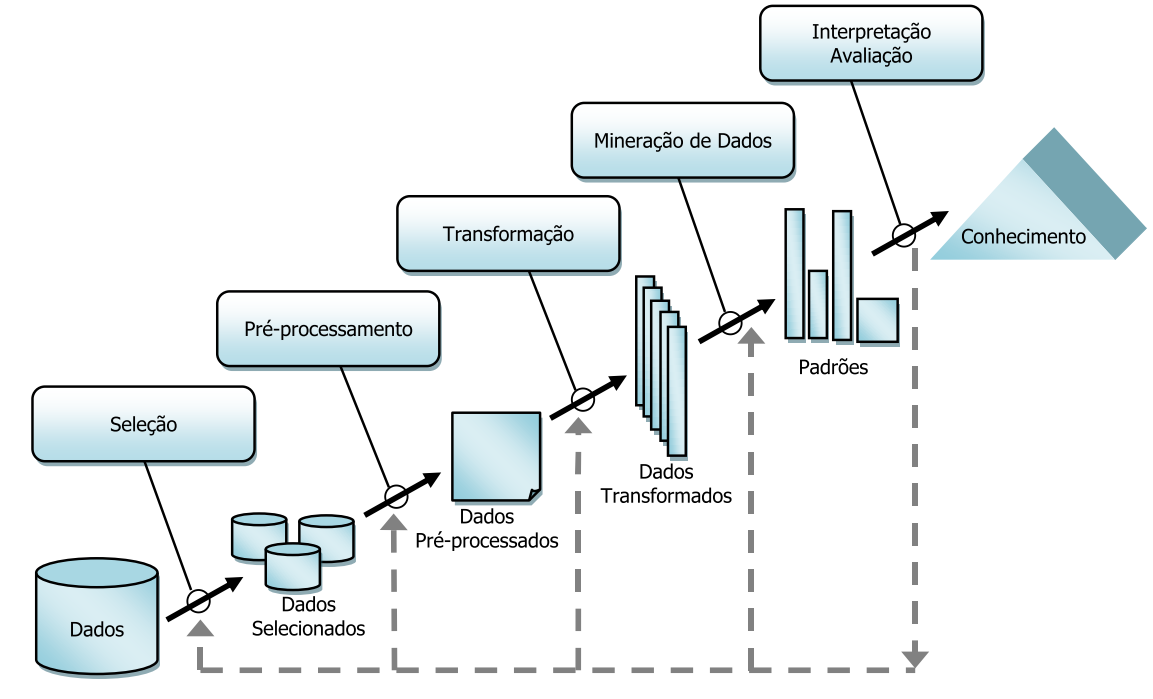
\includegraphics[scale=0.55]{Figuras/Etapas_KDD.png}
	\end{center}
    \legend{Fonte:\cite{Kampff2013}}
\end{figure}

\par
Por tanto ao termino da avaliação, o conhecimento extraído na mineração será introduzido e incorporado por outros sistemas, documentando e disponibilizando os métodos, afim  de apresentar o conhecimento obtido ao usuário ou, mais importante de servir como suporte para a tomada de decisão \cite{Kampff2013}. Resumidamente, essas cinco etapas do processo de KDD podem ser classificadas em três categorias: pré-processamento, mineração de dados e pós-processamento, como é apresentado na Figura 2 \cite{Fayyad1996}.

\begin{figure}[!htp]
	\begin{center}
    \caption{\label{fig:waveform_fig}As três partes da divisão do KDD segundo \cite{Fayyad1996}.}
	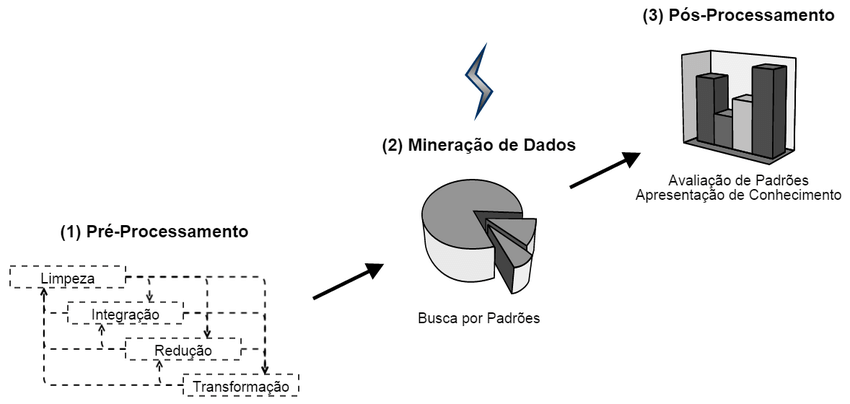
\includegraphics[scale=0.55]{Figuras/Tres_partes_KDD.png}
	\end{center}
    \legend{Fonte:\cite{Maciel}}
\end{figure}

\par
Como vimos antes, a aplicação de KDD, especificamente na etapa de mineração de dados, podemos perceber a sua enorme importância para todas as áreas que necessitem retirar informações de uma base forte e concreta de dados. Com isso, para a próxima seção, serão apresentados os conceitos relacionado a mineração de dados onde será aprofundado mais sobre essa fase explicando sua metodologia e tarefas de mineração.



%==========================
% MINERAÇÃO DE DADOS
%==========================

\section{Mineração de Dados}

O termo Mineração de dados (MD, do inglês, \textit{Data Mining}, DM), conhecido tambem como uma etapa do KDD, pertence a disciplina que tem como objetivo de encontrar novas informações através da análise de grandes volumes de dados. No caso a frase \textbf{novas informações} está se referindo ao processo de reconhecer novos conhecimentos, assim gerando mais descobertas científicas \cite{Baker2011}.

\par
Segundo \citeonline{Amaral2016}, a mineração de dados seria vários processos para explorar e analisar grandes quantidades de dados na busca de padrões, previsões, erros, associações e entre outros. Em outras palavras, as ferramentas de MD examinam os dados, descobrem oportunidades escondidas ou problemas nos relacionamentos dos dados, e então identificam o comportamento dos negócios, envolvendo a mínima interferência do usuário, fazendo com que ele só se dedique a buscar o conhecimento \cite{Jefferson}. 

\par
Comumente a mineração de dados está relacionada a aprendizagem de máquina, que na área de inteligência artificial desenvolve algoritmos capazes de fazer com o que o computador aprenda a partir do passado, isto é, ele aprende utilizando dados de eventos que já aconteceram \cite{Amaral2016}. Pode-se notar, que as ferramentas de mineração são baseados em algoritmos que formam construção de blocos de inteligência artificial, redes neurais e entre outros, que ajuda a facilitar o trabalho de empresas os auxiliando a maximizar os seus lucros \cite{Jefferson}.

\par
Antes ninguém imaginaria que as aplicações de MD seria tão difundida em diversas áreas, pois, muitas delas não possuíam um modelo de dados armazenados digitalmente \cite{Amaral2016}. Hoje existe inúmeras técnicas e tarefas de mineração de dados que vem sendo utilizados com sucesso, em áreas como \textit{marketing} por exemplo, para saber quais produtos um determinado cliente pretende comprar ou em medicina para prever qual paciente vai contrair um certa doença através do seu histórico \cite{Martinhago2005}.

\par
Além de \textit{marketing} e medicina, segundo \citeonline{Amaral2016} a mineração de dados e a aprendizagem de máquina são aplicadas em outras áreas como processamento de linguagem natural, bioinformática, reconhecimento de fala, detecção de fraude,  finanças, sistemas de recomendação, robóticas, mineração de textos, educação e entre outros. No caso, neste trabalho, a mineração de dados educacional será abordado o seu conceito e importância na seção mais a adiante.

\subsection{Tarefas de Mineração de Dados}

\par

As tarefas correspondem aos problemas que podem ser tratados pela mineração de dados. Dependendo do objetivo que se pretende alcançar a seleção da tarefa deve ser feita para se aplicar sobre a base de dados, existem inúmeras tarefas, mas as que são mais utilizadas pela mineração podem ser classificadas como descrição (não-supervisionado) ou predição (supervisionado) \cite{Garcia2013, Camilo2009}.

\par
Segundo \citeonline{Santos2015}, na predição a análise é feita na forma de encontrar padrões repetidos e generalizados, com a finalidade de achar informações que estão escondidos nos dados. Já na descrição, existe argumentos já formulados onde se tenta procurar respostas que confirmem ou neguem esses argumentos, assim, verificando a sua veracidade. As tarefas mais comuns delas, são: 


\subsubsection{Associação}

\par
Uma tarefa de descrição, consiste em determinar quais itens vão ser adquiridos diretamente em uma mesma transação, isto é, quanto um conjunto de atributos favorece para a presença de outro conjunto \cite{Garcia2013}. No caso se X existir alguma transação, há a possibilidade de Y existir também, pode ser apresentado na forma: SE \textit{atributo} X ENTÃO \textit{atributo} Y \cite{Camilo2009}. 

\par
Segundo \citeonline{Camilo2009}, a associação é uma das tarefas mais conhecidas pelo fato de terem tido ótimos resultados, principalmente na área de marketing com a análise de \textbf{Cesta de Vendas}, onde são identificados quais produtos são levados juntos pelo cliente. Pode-se perceber que tais estudos são utilizado para descobrir a relação entre os itens, para assim, criarem pacotes de venda ao consumidor \cite{Garcia2013}. 


\subsubsection{Classificação}

\par
Uma tarefa de predição, consiste em examinar uma certa característica nos dados (\textit{X}) e atribuir uma classe previamente definida (\textit{Y}), ou seja, visa identificar qual classe um determinado registro pertença, como podemos ver representada na Figura 3 \cite{Garcia2013, Kampff2013}. Exemplos disso é classificar se uma pessoa é de renda baixa, média ou alta, ou classificar se um cliente de um banco é bom ou mau pagador, assim determinando se deve conceder ou não créditos ao mesmo.

\begin{figure}[!htp]
	\begin{center}
    \caption{\label{fig:waveform_fig} Associação entre conjuntos de dados e classes.}
	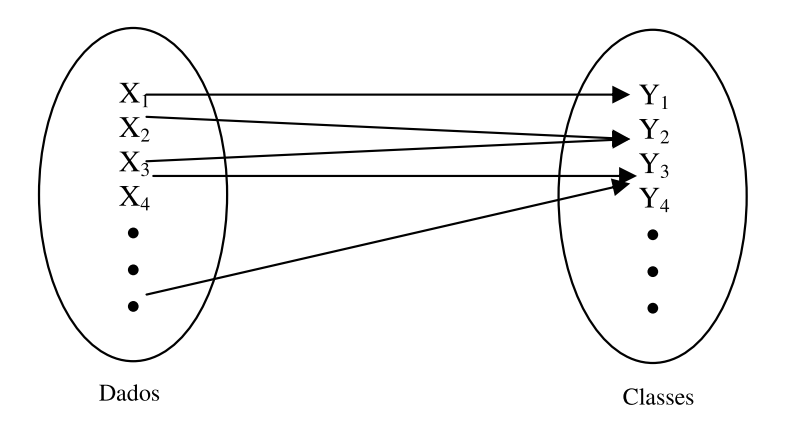
\includegraphics[scale=0.70]{Figuras/Classificacao.png}
	\end{center}
    \legend{Fonte:\cite{Rabelo2007}}
\end{figure}


\subsubsection{Regressão (Previsão ou Estimação)}

\par
Outra tarefa de predição, muito semelhante a anterior, só que com a diferença de que o atributo especial é identificado com um valor numérico e não categórico. Resume-se na estimativa do valor futuro de algum índice se baseando em dados do comportamento passado desse índice \cite{Camilo2009, LeandroSilva2014}. Exemplo, determinar se o índice da BOVESPA subirá ou descerá amanhã, prever o valor de vida de um equipamento, prever o desempenho do aluno, estimar a quantia a ser gasta por uma família de quatro pessoas durante a volta às aulas e entre outros.

\par
A técnica de regressão pode ser classificada em linear e não-linear. Segundo \citeonline{Camilo2009}, são chamados de linear quando tanto as variáveis preditivas quanto as variáveis de resposta possui um comportamento linear em sua relação, por exemplo, quando um valor Y é uma função linear de X representado na Figura 4. Já a não-linear é o oposto da linear, é quando a relação entre as variáveis de resposta e predição não segue um comportamento linear, no caso, as relações entre as variáveis podem ser representadas na forma de uma função polinomial, como demonstrado na Figura 5. 

\begin{figure}[!htp]
	\begin{center}
    \caption{\label{fig:waveform_fig} Gráfico onde o valor y (pontuação alcançada) é uma função linear de x (horas de estudos).}
	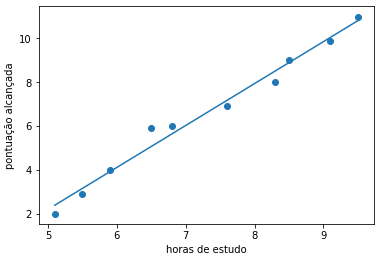
\includegraphics[scale=0.99]{Figuras/Regressao_linear.png}
	\end{center}
    \legend{Fonte:\cite{JoaoPaulo}}
\end{figure}

\begin{figure}[!htp]
	\begin{center}
    \caption{\label{fig:waveform_fig} Gráfico de uma análise de resíduos para modelo de regressão não linear.}
	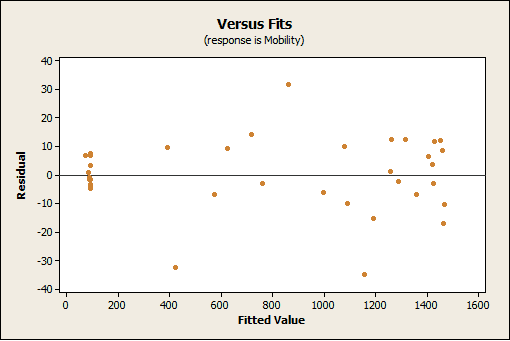
\includegraphics[scale=0.80]{Figuras/Regressao_nao_linear.png}
	\end{center}
    \legend{Fonte:\cite{Paula}}
\end{figure}

\subsubsection{Agrupamento (Clustering)}

\par
Outra tarefa de descrição, é um método de divisão de um conjunto de dados heterogêneos para um grupo homogêneo \cite{LeandroSilva2014}. Ele tende a reconhecer e aproximar os registros similares, isto é, ele junta um conjunto de registro semelhantes entre si que são diferentes de outros registros nos demais agrupamentos \cite{Camilo2009}. \textit{Clustering} difere da classificação, pois, não necessita que os dados sejam previamente classificados (aprendizado não-supervisionado).

\par
Segundo \cite{Camilo2009}, o agrupamento não tem a intenção de predizer, estimar ou classificar uma variável, ele somente reconhece os grupos de dados iguais, como é demonstrado na Figura 6. Alguns exemplos de \textit{clustering} como agrupar clientes por região do país ou com comportamento de compra similar, agrupar alunos com desempenho semelhantes, agrupar seções de usuários Web e entre outros.


\begin{figure}[!htp]
	\begin{center}
    \caption{\label{fig:waveform_fig} Registros agrupados em três \textit{clusters}.}
	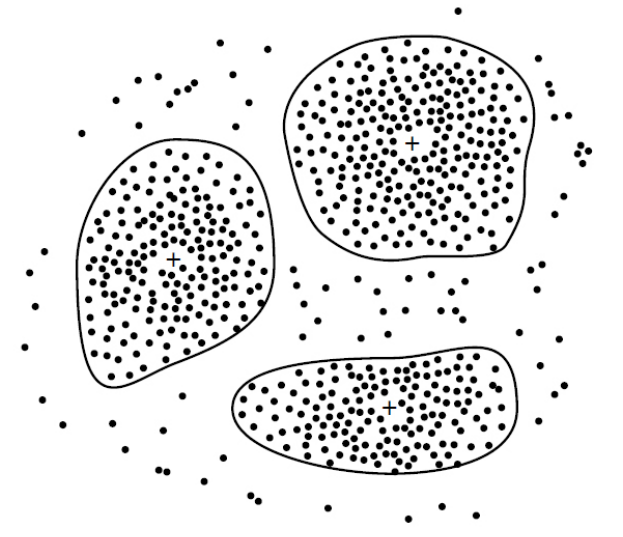
\includegraphics[scale=0.50]{Figuras/Agrupamento.png}
	\end{center}
    \legend{Fonte:\cite{Camilo2009}}
\end{figure}



\subsection{Mineração de Dados e Aprendizagem de Máquina}

\par
Como foi mencionado em tópicos anteriores, podemos perceber que a área de mineração de dados foi favorecida com diversos conceitos provenientes da área de aprendizagem de máquina, muito desses conceitos são vistos em livros voltado para essa área, tais como as técnicas de classificação, regressão, associação e agrupamento. Os dois grupos principais de mineração de dados, predição e descrição, são parecidos com a forma em que os tipos de aprendizagens são divididos: Aprendizagem supervisionada e não-supervisionada.

\par
Por tanto na próxima seção trataremos de alguns conceitos que já foram citados nesse capítulo, sendo que tais conceitos serão estudados de forma mais precisa, voltada para a área de aprendizagem de máquina.

%==========================
% APRENDIZAGEM DE MAQUINA - tecnicas(arvore de decisão, apriori...)
%==========================
\section{Aprendizagem de Máquina}

\par
Existem diversas atividades relacionadas ao conceito de aprendizagem, dificultando ainda mais a exata definição da palavra, tornando assim dependente de contexto. Porém, no contexto computacional, existe uma definição muito precisa de aprendizagem de máquina que pode ser dada \cite{Henke2011}. Segundo \citeonline{Alpaydin2009}, \textit{Machine Learning} são programas de computador que servem para melhorar um processo de um desempenho, utilizando dados de exemplo ou experiência passada.

\par
Em tese, se tem um modelo definido com alguns parâmetros, onde a aprendizagem é aplicada por um programa de computador para poder otimizar o parâmetro desse modelo utilizando dados de treinamento, sendo que, esse modelo pode ser preditivo, descritivo ou os dois \cite{Alpaydin2009}. No caso, a aprendizagem de máquina utiliza o princípio da estatística na elaboração de seus modelos, porque, a tarefa principal está fazendo a dedução a partir de uma amostra. 

\par
Segundo \citeonline{Henke2011}, os algoritmos de aprendizagem podem ser a solução para resolver diversos problemas, pois, eles podem aprender a determinar padrões das classes que estão envolvidas no problema, através de exemplos existentes obtidos do ambiente. Conforme o modelo genérico da Figura 7 sobre aprendizagem de máquina ocorre o seguinte, o ambiente concede a informação para um elemento de aprendizagem, que utiliza essa informação para melhorar a base de conhecimento para que o elemento de desempenho a use na execução de sua tarefa. 

\begin{figure}[!htp]
	\begin{center}
    \caption{\label{fig:waveform_fig} Modelo genérico de aprendizagem de máquina.}
	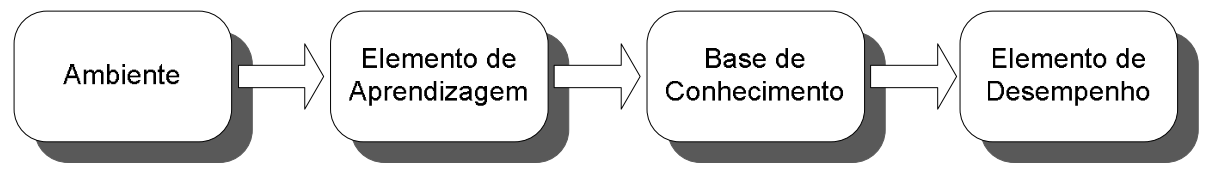
\includegraphics[scale=0.45]{Figuras/Modelo_Machine_Learning.png}
	\end{center}
    \legend{Fonte:\cite{Henke2011}}
\end{figure}

\par
Para a compreensão mais abrangente dos algoritmos de aprendizagem de máquina, é importante conhecer o conceito dos termos mais relevantes e mais usados segundo a nomenclatura abaixo de acordo com \cite{Monard2003, Souto2003, Henke2011}.

\begin{itemize}
    \item \textbf{Exemplo (padrão, instância):} É a ação ou o ato de se pegar um fato que já existe para explicar ou usar para alguma situação (por exemplo, para predição). Na maioria dos casos em aprendizagem de máquina, os exemplos são representados por vetores de características. Um exemplo uma amostra de tecido de um paciente.
    \item \textbf{Característica (atributo, variável):} É utilizado na descrição de um padrão (exemplo). Um atributo possui o seu tipo definido em um domínio, que indica os valores que ele pode apresentar (assumir). Exemplo, nível de expressão de um gene do tecido.
    \item \textbf{Vetor de características:} É quando um exemplo é descrito por uma lista de características. Um exemplo que se pode dar é um vetor m-dimensional que descreve para cada m genes, a medida do tecido de um certo paciente.
    \item \textbf{Classe:} Uma classe contém objetos parecidos, enquanto em outra classe possui objetos diferentes da dela. No caso de aprendizagem supervisionado, todo exemplo sempre possui pelo menos uma variável especial que descreve o fenômeno de interesse. Exemplo, as classes poderiam ser a presença ou a ausência de câncer no tecido.
    \item \textbf{Conjunto de exemplos (conjunto de dados):} É formado por uma quantidade de exemplos (padrões) com seus determinados valores de atributos, onde, em aprendizagem de máquina, cada exemplo é relacionado a uma classe. Geralmente, ele é dividido em dois subconjuntos separados: o conjunto de treinamento e o conjunto de teste.
    \item \textbf{Acurácia (taxa de erro):} Seria a porcentagem de erros ou acertos efetuados pelo modelo para um determinado grupo de dados. No geral, a acurácia é aplicada em testes em que em nenhum momento não foram utilizados durante o processo de aprendizagem. Existem outros meios com técnicas mais complexas na estimação da acurácia como \textit{cross-validation} e \textit{bootstrap}. 
    \item \textbf{Falso positivo:} Suponhamos que temos duas classes, A seria positivo e B negativo, o falso positivo seria a quantidade de exemplos da classe B classificados como da classe A. Já o falso negativo seria o oposto, a quantidade de exemplos A classificados como da classe B. Um exemplo bom onde ocorre isso é em matriz de confusão. 
    \item \textbf{Ruído:} Nenhum conjunto de dados é perfeito, é comum em que qualquer ambiente, acabar trabalhando com dados imperfeitos, no caso esses dados imperfeitos são conhecidos como ruído. Então, ele é definido como um conjunto de dados que aparentemente é inconsistente comparado com o restante dos dados existentes. 
    \item \textbf{\textit{Overfitting} (super-ajustamento):} É um termo que é utilizado para descrever quando um modelo se ajusta (especializa) muito bem ao conjunto de dados utilizados no seu treinamento, mas se torna ineficaz para prever novos resultados demonstrando uma taxa de acurácia baixa.
\end{itemize}

\subsection{Tipos de Aprendizagem}

\par
Segundo \citeonline{Henke2011} a aprendizagem de máquina pode ser dividido em dois tipos principais de aprendizagem: aprendizagem supervisionada e aprendizagem não-supervisionada.

\subsubsection{Aprendizagem Supervisionada}

\par
Conhecido também como aprendizagem com o professor, nele se tem a figura de um professor externo, no qual apresenta o conhecimento do ambiente através de um conjunto de exemplos de pares de entrada e saída, onde são propagados em uma sequência de regras que a máquina acompanhara para se obter o efeito desejado \cite{Lorena2007, Henke2011}.

\par
Exemplos desse tipo de aprendizagem, no caso de regressão, dado uma imagem de uma pessoa, através dos dados da imagem fornecido temos que prever a sua idade. Em classificação, dado um exemplo de tumor cancerígeno, temos que prever através da idade e do tamanho do tumor do paciente se ele é maligno ou benigno \cite{Pedro}.

\subsubsection{Aprendizagem Não-Supervisionada}

\par
Nesse não existe a presença de um professor, ou seja, não há exemplos rotulados de alguma função para ser aprendida \cite{Lorena2007, Henke2011}. Nessa aprendizagem são identificados dois tipos de subdivisão:

\begin{itemize}
    \item \textbf{Aprendizagem por reforço:} Não se sabe qual a saída correta. Ele se preocupa de como um agente deve agir em um ambiente de forma que potencialize alguma noção de recompensa a longo tempo. Como os pares de entrada e saída não são fornecidos, ele tenta encontrar uma maneira de mapeá-los através de uma interação contínua com o ambiente, para poder reduzir um índice escalar de desempenho \cite{Henke2011, Alpaydin2009}. 
    \item \textbf{Aprendizagem não-supervisionada:} Não existe padrões de saída desejada. O algoritmo aprende a agrupar ou representar as entradas submetidas de acordo com uma medida de qualidade. Esse tipo de aprendizagem é usada principalmente quando se quer encontrar padrões ou tendências que ajudem na compreensão dos dados, nela inclui estimação de densidade, formação de agrupamentos e dentre outros \cite{Henke2011, Lorena2007}.
\end{itemize}

\par
Exemplo de aprendizagem não-supervisionada, no caso de agrupamento, dado um determinado conjunto de 1000 pesquisas de uma universidade, queremos encontrar um jeito de agrupar automaticamente elas de acordo com suas semelhanças ou relações por diferentes variáveis, tais como frases, sequências das palavras, contagens de páginas e etc \cite{Pedro}. Já na aprendizagem por reforço, temos como exemplo jogos, robôs e navegação.


\subsection{Algoritmos de Aprendizagem}

\par
Existe uma extensa quantidade de algoritmos disponíveis para classificação, regressão e associação em aprendizagem de máquina, sendo que serão falados apenas alguns dos principais que são mais utilizados. Todos os algoritmos que serão mencionados abaixo, podem ser utilizados tanto para classificação quanto para regressão. %\textcolor{red}{Avore de decisão - supervisionado, KNN - supervisionado, redes neurais - supervisionado, naive bayes - supervisionado, SVM - supervisionado.}


\subsubsection{Árvore de Decisão}

\par
Árvore de decisão (\textit{Decision Trees}) é uma ferramenta de aprendizagem que pode ser utilizada para tomada de decisão e dedução de valores categóricos. A ideia é de um aprendizado indutivo: se cria uma hipótese constituída em instâncias específicas que gera conclusões gerais \cite{Marques2014}. As árvores de decisão pegam como entrada um caso representado por um conjunto de atributos que retorna a uma decisão, que é a categoria para o valor de entrada


\par
Uma árvore é composta por três elementos importantes: os nós internos representam diferentes características, os ramos entre esses nós representam a possíveis valores que essas características podem possuir, enquanto os nós folhas representam o resultados, no caso, os valores de classificação da aplicação \cite{Henke2011, Barros2012}. Segundo \citeonline{Barros2012}, para a realização da classificação, deve ter uma tupla correspondente às características dos fluxos, que percorre pela árvore do nó raiz até  todos os nós folhas.  

\par
Para o melhor entendimento do processo de classificação de uma árvore de decisão, a Figura 8 mostra um exemplo usado no treinamento de dados para a tarefa de detecção de intrusão. De início, uma base de dados é fornecida ao algoritmo, onde, ele gera uma árvore feita para separar as amostras da classe Maligna de amostras da classe Benigna. Depois da construção da árvore, os dados novos podem ser fornecidos ao classificador, ao qual concedera uma das duas classes à amostra testada \cite{Henke2011}. 

\begin{figure}[!htp]
	\begin{center}
    \caption{\label{fig:waveform_fig} Treinamento dos dados em uma Árvore de Decisão.}
	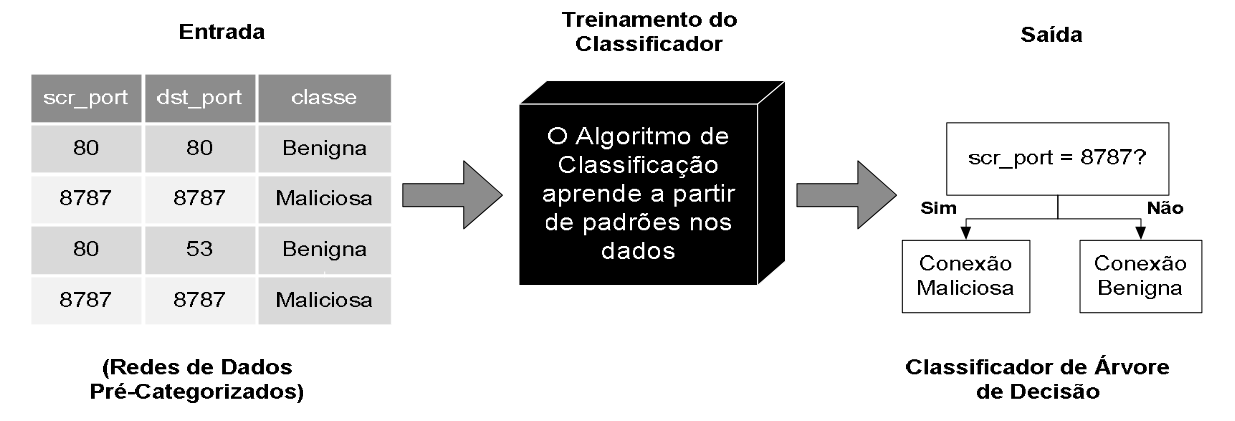
\includegraphics[scale=0.50]{Figuras/Arvore_decisao.png}
	\end{center}
    \legend{Fonte:\cite{Henke2011}}
\end{figure}

\par
Pelo que podemos perceber em um ponto de vista de decisão de negócios, uma árvore de decisão é uma quantidade mínima de perguntas sim ou não que alguém tem que perguntar, para poder avaliar a possibilidade de fazer uma decisão correta a maior parte do tempo. Como ferramenta, possibilita tratar o problema de forma estruturada e sistemática para chegar a uma conclusão lógica \cite{Sara}. 


\subsubsection{K-\textit{Nerarest Neighbor} (KNN)}

\par
O algoritmo de KNN ou K-Vizinho Mais Próximo é um potente algoritmo não-paramétrico de classificação e regressão, utilizado desde 1950 na área da estatística \cite{Carvalho2014}. Segundo \citeonline{Henke2011}, ela é uma técnica baseada em instâncias, que constitui em atribuir a classe de cada elemento novo a partir da classe dominante conseguida através de seus vizinhos mais próximos, detectado no conjunto de treinamento. A definição de vizinhança é feita segundo a uma medida de distância estimado no espaço de atributos, exemplo de medida é a Euclidiana. 

\par
Por exemplo, queremos determinar a renda de uma pessoa de uma região, pesquisando k=20 vizinhos mais próximos desse indivíduo, podemos obter a renda através de valores dos atributos bairro, moradia, profissão, escolaridade e idade. Um de alguns problemas dessa técnica é a necessidade de se ter um número de atributos bastante razoável para a determinação da vizinhança, e também, esse processo de classificação pode ser bastante cansativo para a máquina quando o conjunto de treinamento tem bastante dados \cite{Cortes2002, Henke2011}.

\subsubsection{Naive Bayes}

\par
Essa técnica de aprendizagem de máquina se baseia em fundamentações simples, mas que constantemente gera uma alta taxa de classificação em questões reais, como por exemplo, uma resposta para tal questionamento, como, qual a chance de um ataque ser de um determinado tipo, dado alguns acontecimentos do sistema observado? \cite{Henke2011}. Segundo \citeonline{Barros2012}, naive bayes analisa as categorias de aplicação para cada instância e relações dos atributos, derivando a probabilidade para cada relação delas entre seus valores.

\par
Segundo \cite{Henke2011}, uma de suas principais vantagens é a baixa complexidade na fase de treinamento, sendo que essa fase envolve somente os cálculos de frequência para que as probabilidades sejam conseguidas. Em aplicações \textit{online}, como problemas envolvendo segurança de redes, cujo, treinamento deve ocorrer online e com frequência continua, por ela ter essa característica naive bayes é muito indicada. Outra característica importante para segurança de redes, é o fato de ela poder manipular atributos nominais e numérico.

\par
O modelo de Naive Bayes é simples de construir e principalmente útil para grandes volumes de dados. Além de fácil, ele é conhecido também por ganhar de técnicas de classificação que são mais sofisticadas \cite{Sunil}. Naive Bayes utiliza o teorema de bayes que fornece uma forma de calcular a probabilidade posterior P(A|B) a partir de  P(A|B), P(A) e P(B). Observe a \autoref{eq:Bayes} abaixo:

\begin{equation}
    \label{eq:Bayes}
        {P(A|B)\quad =\frac { P(B|A)\quad *\quad P(A) }{ P(B) } }
\end{equation}

\par
Segundo \citeonline{Thiago}, precisamos dos seguintes dados utilizado na \autoref{eq:Bayes}, que são:
\begin{itemize}
    \item \textbf{P(A|B):} É a probabilidade posterior da classe (B, alvo) dada preditor (A, atributos), ou seja, a probabilidade de A acontecer dado que B ocorreu.
    \item \textbf{P(B|A):} É a probabilidade que representa a probabilidade de preditor dada a classe, ou seja, a probabilidade de B acontecer dado que A ocorreu.
    \item \textbf{P(A):} É a probabilidade original da classe, ou seja, a probabilidade de A ocorrer.
     \item \textbf{P(B):} É a probabilidade original do preditor, ou seja, a probabilidade de B ocorrer.
\end{itemize}

\subsubsection{Redes Neurais}

\par
Redes Neurais é uma técnica originado da psicologia e neurobiologia, que compõe basicamente de simulações baseada no comportamento dos neurônios \cite{Camilo2009}. Tal ideia vem da seguinte razão: o cérebro é tipo um aparelho que processa a informação com inúmeras habilidades, tais como por exemplo, o reconhecimento de voz, visão e etc. Por tanto, uma rede neural é bastante conectada por várias unidades (nó) como os neurônios, do qual a saída é uma combinação de várias entradas para outros neurônios \cite{Henke2011, Barros2012}.

\par
Segundo \cite{Carvalho2014}, na área de aprendizagem de máquina os algoritmos de redes neurais artificial são considerados poderosos, sendo que, são usados na resolução de problemas lineares e não-lineares, tendo apoio tanto no aprendizado supervisionado quanto no não supervisionado. Sua utilização mais constante é na solução de problemas não-lineares de classificação, através de uma estrutura conhecida com \textit{Multi-Layer Perceptron} (MPL) que sempre trabalha em conjunto nessa área de aprendizagem com o algoritmo mais conhecido, o algoritmo de Retropropagação (\textit{Backpropagation)}.

\par
Em bases de dados que possuam muitos ruídos, que no caso são as inconsistências encontradas no conjunto de dados de treinamento, a técnica de redes neural é bastante recomendada. Pois, eles conseguem ser relativamente quase imunes a este ruídos, diferentes de outros modelos de aprendizagem supervisionado como árvore de decisão que são severamente afetados por esses ruídos \cite{Carvalho2014}. A Figura 9 logo depois, apresenta as diversas camadas que podem ser criadas em um processamento de uma rede neural \cite{Cortes2002}.

\begin{figure}[!htp]
	\begin{center}
    \caption{\label{fig:waveform_fig} Representação de um processamento de uma rede neural.}
	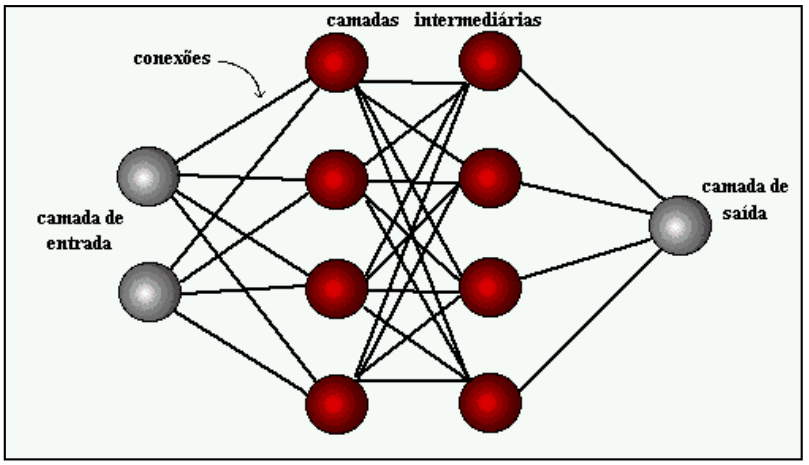
\includegraphics[scale=0.56]{Figuras/Redes_neural.png}
	\end{center}
    \legend{Fonte:\cite{Cortes2002}}
\end{figure}

\par
Segundo \citeonline{Cortes2002}, apresentado na Figura 8, todas as camadas intermediárias simbolizam os diferentes níveis de conhecimento que são obtidos no processo de seu percurso, numa tentativa de copiar o cérebro humano. Apesar de ser uma técnica poderosa, redes neurais é pouco utilizado em mineração de dados, pelo fato de seus algoritmos serem em sua maioria, incompreensíveis e também a função de aprendizado ser consideravelmente lenta, devido as várias interações que o algoritmo de retropropagação realiza para atualizar os valores da rede \cite{Carvalho2014}. 



\subsubsection{\textit{Support Vector Machines} (SVM)}

\par
Máquina de vetores de suporte é um algoritmo supervisionado que é usado para o trabalho de classificação, onde ele utiliza um hiperplano como separador de classes. Este hiperplano é encontrado através da utilização do conjunto de treinamento (vetores de suporte) e ele trabalha como uma base para o limite da decisão ao classificar \cite{Costa2012}. Segundo \citeonline{Henke2011}, ela é uma técnica de classificação bastante aplicada em problemas de segurança, como por exemplo na detecção de \textit{phishing} e detecção de intrusos.

\par
O funcionamento do SVM pode ser dito da seguinte forma: se tem duas classes e um conjunto de treinamento onde as amostras pertencem as classes, a máquina vetor de suporte cria um hiperplano (conhecido como hiperplano de separação ótima) que divide o espaço de atributos em duas regiões, potencializando a margem de separação entre as mesmas. As amostras que antes não eram conhecidas são mapeadas para esse mesmo espaço e depois atribuídas a uma das classes \cite{Henke2011}.


\par
Como exemplo na Figura 10, suponhamos que os dados de treinamento sejam referentes aos alunos de uma turma com suas informações, apresentados como pontos, como a quantidade de postagens em um fórum de discussão (variável preditora). Além que, os dados representam cada aluno conforme o seu desempenho na disciplina (variável preditiva), alunos que passaram (pontos brancos) e que reprovaram (pontos pretos). A priori, a meta do SVM é encontrar a melhor maneira de separar os dois grupos de alunos \cite{Costa2012}.


\begin{figure}[!htp]
	\begin{center}
    \caption{\label{fig:waveform_fig} Dados de treinamentos representando alunos que passaram (pontos brancos) e não passaram (pontos pretos) em uma disciplina.}
	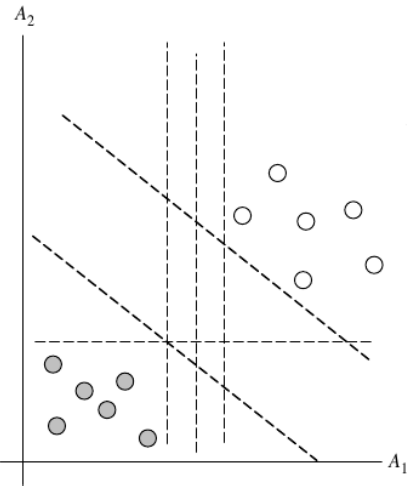
\includegraphics[scale=0.50]{Figuras/SVM.png}
	\end{center}
    \legend{Fonte:\cite{Costa2012}}
\end{figure}

\begin{figure}[!htp]
	\begin{center}
    \caption{\label{fig:waveform_fig} Representação do melhor hiperplano que separa as classe, encontrado pelo algoritmo de SVM.}
	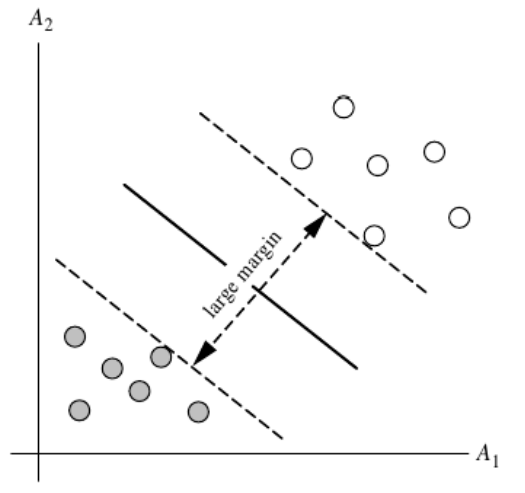
\includegraphics[scale=0.50]{Figuras/SVM_2.png}
	\end{center}
    \legend{Fonte:\cite{Costa2012}}
\end{figure}

\par
Pode-se notar que existe uma quantidade infinita de hiperplanos que são representas na Figura 10 como essas linhas tracejadas, que podem separar as classes demonstradas que no caso são os círculos brancos e círculos cinzas. Então o propósito da máquina vetor de suporte é de encontrar o melhor hiperplano que maximize a distância entre elas das classes vizinhas. Um exemplo do melhor hiperplano para os dados que foram mostrado na Figura 10 encontrado pelo SVM é apresentado na Figura 11 \cite{Costa2012}. 


\par
Embora SVM seja uma técnica recente, ela tem atraído muita atenção pelos seus resultados como: a possibilidade de modelar casos não-lineares difíceis gerando modelos de simples compreensão, consegue altos índices de assertividade, pode ser usada tanto para relações lineares quanto relações não lineares e entre outros \cite{Camilo2009}. Ultimamente um dos problemas dessa técnica é o tempo que se usa no aprendizado e muitas pesquisas estão se concentrando neste aspecto. 


\subsubsection{Apriori}

\par
O algoritmo apriori, é um dentre os algoritmos mais utilizados para mineração por regras de associação. Este algoritmo utiliza busca por profundidade e gera um conjunto de itens padrões (candidatos) de k elementos a partir de itens k-1 elementos. Os itens candidatos que não são frequentes são excluídos. Tudo da base de dados é rastreada e a partir dos conjuntos de itens candidatos, os itens frequentes são obtidos \cite{Vasconcelos2004}. Além disso, o algoritmo possui vários atributos que otimizam o seu desempenho, uma delas é antmonotonia da relação, que diz que para cada \textit{itemset} ser frequente, todos do seu subconjunto devem ser também, além de usar estrutura hash e recursos da memória principal.

\par
Segundo \citeonline{Romao1999}, o algoritmo apriori possui três processos que é a geração dos conjuntos de candidatos, a poda dos conjuntos dos candidatos e a contagem de suporte que seria no caso a extração de regras de associação. A propriedade antmonotonia do algoritmo apriori poderia ser explicado da seguinte forma, se X está contido Y e X não é um \textit{itemset} frequente, logo o Y também não será frequente. Isso evita uma grande quantidade de tempo de execução, pois, se X não é frequente, não há a necessidade de calcular o suporte de Y e o todo o banco de dados não precisará ser verificado.

%==========================
% PARAMETROS
%==========================

\section{Parâmetros Utilizados Para Classificação e Associação}

\subsection{Suporte, Confiança e Lift}

\par
\textcolor{red}{Na associação, o método para se encontrar as regras para ela pode ser dividido em duas partes. A primeira é a de descobrir todos os \textit{itemset} (conjunto de itens) que possuam um suporte com transações igual ou superior ao limite mínimo que foi especificado, onde os itens encontrados são conhecidos como o conjunto de itens frequentes, e a segunda parte é a de gerar as regras de associação a partir dos \textit{itemset} frequentes encontrados, no qual, serão selecionado apenas as regras que possuam um grau de confiança mínima especificado pelo usuário \cite{Vasconcelos2004, LeandroSilva2014}.}

\textcolor{red}{Praticamente, dado um conjunto de transações, o objetivo em minerar por regras de associação é a de encontrar todas as regras que possuam o suporte e a confiança iguais ou superiores ao valores minimo especificado pelo úsuario \cite{Vasconcelos2004}. O suporte de uma regra X $\rightarrow$ Y, onde X e Y são  \textit{itemset}, é dada pela seguinte fórmula apresentada na \autoref{eq:Suporte}:}


\begin{equation}
    \label{eq:Suporte}
        {\textit{Suporte}\quad =\frac { \textit{Frequência de X e Y} }{ \textit{Total de T}} }
\end{equation}

\par
\textcolor{red}{A fórmula pode ser interpretada da seguinte maneira, o numerador representa a quantidade de transações que ocorrem simultaneamente tanto para X quanto para Y e o denominador representa o total de transações a qual aquele conjunto pertence. Já para a confiança, é dada pela seguinte fórmula que é demonstrada na \autoref{eq:Confianca}:}

\begin{equation}
    \label{eq:Confianca}
        {\textit{Confiaça}\quad =\frac { \textit{Frequência de X e Y} }{ \textit{Frequência de X}} }
\end{equation}

\par
\textcolor{red}{Na fórmula acima, o numerador representa a quantidade de transações em que X e Y ocorrem simultaneamente e o denominador representa a quantidade de transações que o item X ocorre. No caso, o suporte (\autoref{eq:Suporte}) pode ser retratado como a probabilidade em que uma transação qualquer satisfaça tanto X quanto Y e na confiança (\autoref{eq:Confianca}) é a probabilidade que uma transação qualquer satisfaça Y, dado que ela ocorra em X.}

\begin{figure}[!htp]
	\begin{center}
    \caption{\label{fig:waveform_fig} Tabela do exemplo da base de dados de um supermercado.}
	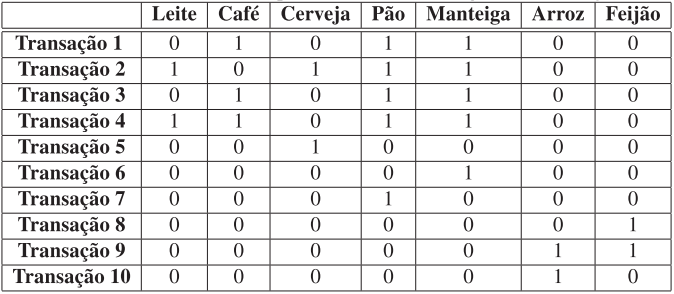
\includegraphics[scale=0.80]{Figuras/Tabela_da_base_de_supermercado.png}
	\end{center}
    \legend{Fonte:\cite{Vasconcelos2004}}
\end{figure}

\par
\textcolor{red}{Para entender melhor esse processo, vamos pegar o exemplo que \citeonline{Vasconcelos2004} demonstraram. Conforme a Figura 12 representada acima, que demonstra uma tabela referente a base de dados de um supermercado, as colunas correspondem aos itens e as linhas correspondem as transações, os valores 0 e 1 representam a presença daquele item na transação correspondente, no caso, 0 refere-se a ausência do item e 1 refere-se a presença do item. O suporte mínimo especifica para o exemplo e de 30\% (0.3) e a confiança mínima é de 80\% (0.8).} 



\textcolor{red}{Os autores \citeonline{Vasconcelos2004} consideraram X = {Café} e Y = {Pão} e calcularam o suporte e a confiança para o conjunto {Café, Pão}. Ao verificarem na tabela, eles observaram que em apenas 3 transações (transação 1, 3 e 4) os dois itens aparecem com o valor 1 simutaneamente. Desa forma, pegando a fórmula do suporte que é apresentado na \autoref{eq:Suporte}, o numerador recebe o valor 3 (que foi a quantidade das transações em que os dois itens ocorreram ao mesmo tempo) e o denominador recebe o valor 10 (que é o numero total de transações ocorridas). Logo obtiveram, Suporte = 3/10 = 0.3 (30\%).}

\par
\textcolor{red}{Para a confiança, \citeonline{Vasconcelos2004} pegaram os mesmos itens (Café, Pão) que foram comprovados que eles possuem um suporte igual ou superior que 30\%, o calculo foi feito da seguinte forma: o numerador recebeu o mesmo valor que foi obtido no numerador da equação do suporte que é 3 e o denominador recebeu a quantidade de transações que os itens de X possuem como valor 1 em relação a transação total (10 transações), logo ele recebe o valor como 3. Portanto, Confiança = 3/3 = 1 (100\%). Logo, a regra gerada Café $\rightarrow$ Pão (se o cliente compra café, então ele compra pão) ocorre com 100\% das transações (compras efetuadas).}

\par
\textcolor{red}{Uma observação que tem que ser feita, é que o cálculo do suporte é feito para todos os conjuntos de itens que ocorrem na mesma transação, desde a quantidade mínima de itens até o conjunto da quantidade máxima de itens. No caso, pegando os dados do supermercado utilizado, como é apresentado na figura da tabela mostrado anteriormente, o mínimo do conjunto de itens é de 1 e o máximo do conjunto itens é de 4 que ocorrem na mesma transação, como é o caso da transação 4 (Leite, Café, Pão, Manteiga). Em casos onde é gerado uma grande quantida de regras que possuam um valor de confiança igual ou surperior ao que foi determinado, para saber quais entre elas é a melhor regra, é recomendado que utilize a medida de interesse Lift.}

\par
\textcolor{red}{Segundo \citeonline{Gonsalves2004}, o lift é uma métrica de avaliação de regras de associação que demonstra para cada regra gerada o grau de relevância dela, podendo assim, fazer uma filtragem das mais relevantes. A fórmula do lift funciona da seguinte forma, como apresentado na \autoref{eq:Lift}:}

\begin{equation}
    \label{eq:Lift}
        {\textit{Lift (X $\rightarrow$ Y)}\quad =\frac { \textit{Confiança (X $\rightarrow$ Y)} }{ \textit{Suporte de Y}} }
\end{equation}

\par
\textcolor{red}{O numerador representa o valor de confiança da regra que foi obtida X $\rightarrow$ Y e o denominador representa o valor de suporte obtido de Y. No caso, o lift pode ser tratado como o qual mais frequente se torna Y quando X $\rightarrow$ Y ocorre \cite{Gonsalves2004}. Para esclarecer melhor, ainda com o exemplo dosupermercado, determinamos um lift maior ou igual a 2, pegando pelo menos 3 regras que passaram de 80\% de confiança: Café $\rightarrow$ Pão com 100\%, Café $\rightarrow$ Manteiga com 100\% e Pão $\rightarrow$ Manteiga com 80\%. E pegando tambem os suporte de pão e manteiga com 50\%. Logo, temos o seguinte:}

\textit{Lift (Café $\rightarrow$ Pão)} = \textit{Confiança (Café $\rightarrow$ Pão)} /  \textit{Suporte (Pão)} = 1 / 0,5 = 2
    
\textit{Lift (Café $\rightarrow$ Manteiga)} = \textit{Confiança (Café $\rightarrow$ Manteiga)} /  \textit{Suporte (Manteiga)} = 1 / 0,5 

= 2
    
\textit{Lift (Pão $\rightarrow$ Manteiga)} = \textit{Confiança (Pão $\rightarrow$ Manteiga)} /  \textit{Suporte (Manteiga)} = 0,8 / 0,5 

= 1,6


\par
\textcolor{red}{}


\subsection{Entropia e Ganho de Informação}

\par
\textcolor{red}{Na classificação, o processo da escolha dos atributos mais relevantes para a construção de uma árvore de decisão é feito por dois métodos de seleção: Entropia da informação e Ganho de informação.}

\par
\textcolor{red}{A Entropia da Informação é a medida utilizada para indicar a homogeneidade dos exemplos contidos em um conjunto de dados, ou seja, ela calcula a impureza em um determinado subconjunto \cite{Carvalho2014}. Através dessa métrica, é possível diminuir a quantidade de informação necessária para classificar um determinado registro, garantindo assim, que uma árvore simplificada seja obtida. A formula da entropia é demonstrado na \autoref{eq:Entropia}:}

\begin{equation}
    \label{eq:Entropia}
        {\textit{Entropy(S)}={\sum_{i=1}^{C} -(p_i)\log_{2}(p_i)}}
\end{equation}

\textcolor{red}{Dado um conjunto de entrada (S) que pode ter \textit{C} classes distintas (número de classes), onde $p_i$ é a proporção de dados em S que pertencem á classe i. O logaritmo de base 2 é utilizado pelo fato que a medida da entropia é em \textit{bits}.}

\par
\textcolor{red}{Já o Ganho de Informação é a medida utilizada para determinar o quanto um dado atributo irá particionar (dividir) os exemplos de aprendizado de acordo com sua função objetivo (classes), ou seja, é o ganho de informação obtido ao dividir o conjunto de dados com base no atributo calculado, determinado pela diferença entre a entropia original e a entropia calculada após a divisão (particionamento) do conjunto \cite{Carvalho2014, Steiner2004}. A formula do Ganho de informação é representada na \autoref{eq:Ganho}:}

\begin{equation}
    \label{eq:Ganho}
        {\textit{Gain(S,A)}={\textit{Entropy(S)} -  \sum_{v \in Values(A)} \frac{|S_v|}{|S|} Entropy(S_v) } }
\end{equation}

\par
\textcolor{red}{A \textit{Entropy(S)} representa a entropia original (classes da variável dependente), no caso, a entropia das classes da variavel dependente (Aprovado:Sim ou Não), \textit{Values(A)} representa os conjunto dos valores que A pode assumir, \textit{v} um elemento deste conjunto e $S_v$ o subconjunto de S formado pelos dados em que A=v. Sendo que \textit{Entropy(S)} é uma medida de homogeneidade  dos exemplos contidos em um conjunto de dados (S), \textit{Values(A)} é uma medida de homogeneidade estimada para o
conjunto S caso utilize o atributo A para fazer a próxima partição.}

\par
\textcolor{red}{A construção de uma árvore de decisão tem três objetivos, quais sejam: diminuir a entropia (a aleatoriedade da variável objetivo), ser consistente com o conjunto de dados e possuir o menor número de nós \cite{Steiner2004}. Para melhor entendimento dos cálculos acima, será utilizado o exemplo do jogar tênis para ilustrar. Como demonstrado na Tabela 1, os conjuntos de atributos tempo, temperatura, umidade e vento que auxiliam na decisão de jogar tênis (sim ou não).}

\par
\begin{table}[!htp]
	\begin{center}
    \caption{\label{fig:waveform_fig} Base de treinamento do jogo tênis.}
	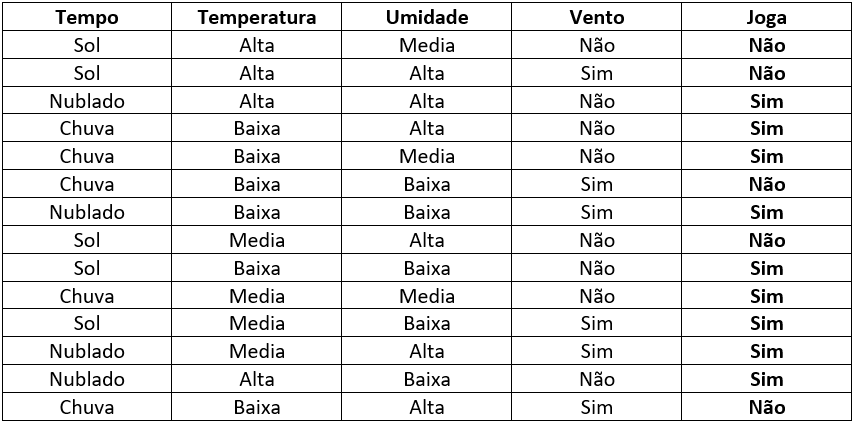
\includegraphics[scale=0.65]{Figuras/Jogar_tenis.png}
	\end{center}
\end{table}

\par
\textcolor{red}{Primeiramente calculamos a entropia original para a variável dependente Joga, em relação as suas duas classes ao total de registros da variável a que elas pertencem, no caso, a classe Sim possui 5 registros e classe Não possui 9 registros dentre os 14 registros no total, como demonstrado o cálculo abaixo:}

\textit{Entropy(Joga)}={ - ($\frac{5}{14}$)$\log_{2}$($\frac{5}{14}$) - ($\frac{9}{14}$)$\log_{2}$($\frac{9}{14}$) = 0,16 + 0,12 = 0,28.}

\par
\textcolor{red}{Em seguida, calculamos a entropia das classes pertencente a variável Joga em relação a quantidade de vezes que cada uma das classes do atributo Tempo aparecem. No caso, o valor Sol possui 5 registros contendo 2 registros com a classe Sim e 3 registros com a classe Não, o valor Nublado possui 4 registros contendo os 4 registros somente para a classe Sim e o valor Chuva possui 5 registros contendo 3 registros para a classe Sim e 2 registros para a classe Não. Como demonstrado o cálculo abaixo:}

\textit{Entropy(Joga,Sol)}={ - ($\frac{2}{5}$)$\log_{2}(\frac{2}{5})$ - ($\frac{3}{5}$)$\log_{2}(\frac{3}{5})$ = 0,16 + 0,13 = 0,29}

\textit{Entropy(Joga,Nublado)}={ - ($\frac{4}{4}$)$\log_{2}(\frac{4}{4})$ = 0}

\textit{Entropy(Joga,Chuva)}={ - ($\frac{3}{5}$)$\log_{2}$($\frac{3}{5}$) - ($\frac{2}{5}$)$\log_{2}$($\frac{2}{5}$) = 0,13 + 0,16 = 0,29} 

\par
\textcolor{red}{Depois de fazer o cálculo da entropia para cada valor da variável Tempo, aplicamos os resultados deles ao cálculo de ganho de informação, onde o valor da entropia original é subtraído pela soma da quantidade de vezes em que o valor do registro apareceu dividido pelo total de registros da sua variável pertencente sendo multiplicado pela sua respectiva entropia. No caso, a variável tempo possui 14 registro no total, contendo 5 registros para o valor Sol possuindo o valor de entropia de 0,29 em relação as classes da variável Joga, 4 registros para o valor Nublado com o valor de entropia de 0 e 5 registros para o valor Chuva com o valor de entropia de 0,29, como demonstrado logo abaixo:}

\textit{Gain(Joga,Tempo)}={ 0,28 - ($\frac{5}{14}$).0,29 - ($\frac{5}{14}$).0 - ($\frac{5}{14}$).0,29 = 0,28 - 0,1 - 0 - 0,1 = 0,08} 
\par
\textcolor{red}{Para facilitar o entendimento do que foi feito, a Figura 13 apresenta o passo a passo do que foi feito:}

\begin{figure}[!htp]
	\begin{center}
    \caption{\label{fig:waveform_fig} Demonstração do cálculo da Entropia e do Ganho de informação.}
	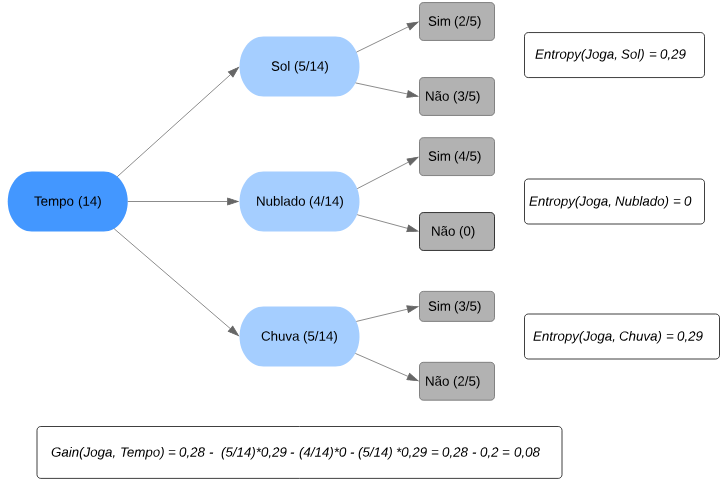
\includegraphics[scale=0.80]{Figuras/Calculo_ganho_de_informacao.png}
	\end{center}
    \legend{Fonte:Próprio autor.}
\end{figure}

\par
\textcolor{red}{Fazendo o mesmo cálculo para os outros atributos a taxa de ganho obtido foi: 0,02 para temperatura, 0,01 para umidade e 0,02 para vento. Analisando com o resultado que já foi obtido do ganho de informação do atributo Tempo (0,08), percebemos que o atributo Tempo possui a taxa de ganho mais alta, logo, se for utilizado somente o atributo Tempo, terá uma alta probabilidade de se obter uma classificação mais interessante para a árvore. Logo, o atributo Tempo vai estar na raiz da árvore de decisão.}

\par
\textcolor{red}{A partir da raiz da variável Tempo, dependendo do ramo que for percorrido o cálculo de entropia e ganho de informação é aplicado para aquele caminho e sucessivamente para todos os ramos até gerar a arvore toda. Ou seja, o valor (ramo) Sol possui 5 atributos, o cálculo do ganho de informação dos outros atributos em relação a variável dependente Joga, vai estar sendo limitado por 5 registros apenas, como demonstrado na Tabela 2:}

\par
\begin{table}[!htp]
	\begin{center}
    \caption{\label{fig:waveform_fig} Registros do valor Sol.}
	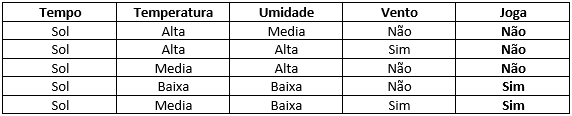
\includegraphics[scale=0.90]{Figuras/Ramo_sol.png}
	\end{center}
\end{table}

\section{Validação do Modelo}

\par
\textcolor{red}{Na implementação ou utilização de um algoritmo, é essencial verificar a sua precisão (acurácia) em um conjunto de teste. Por exemplo, em classificação, no caso da árvore de decisão que são propenso ao problema denominado como \textit{overfitting}, onde, a árvore gerada não consegue generalizar corretamente novas instâncias de testes, possuindo uma capacidade de predição muito abaixo da precisão desejada ao se utilizar o conjunto de teste de dados de treinamento \cite{Carvalho2014}. Para evitar este tipo de problema, avaliando a estimativa de erro obtida pela árvore, pode se utilizar algumas técnicas como: \textit{cross-validation} e matriz de confusão.}



\subsection{Cross-Validation}

\par
\textcolor{red}{A validação cruzada é uma técnica que avalia a eficiência de generalização de um modelo a partir de um conjunto de dados, ou seja, ela analisa se o conjunto de dados de treinamento é representado o bastante em relação à base de dados na qual se deseja predizer certas instâncias \cite{Carvalho2014, Monard2003}.}

\par
\textcolor{red}{O método mais comum de ser utilizado é o K-partições, onde, por exemplo utilizando k = 10 \textit{folds}, ele pega uma base inteira e a divide em 10 partições com a mesma quantidade de instâncias (aqueles que não são divisível pelo valor definido, o restante que sobra são distribuídas pelas partições), sendo que em 10 interações, para cada partição será o conjunto de teste enquanto as 9 restantes serão utilizadas como conjunto de caso de treinamento \cite{Carvalho2014}.}

\par
\textcolor{red}{A cada interação realizada, é calculada a estimativa de erro do modelo (que é a quantidade de vezes em que foi classificado incorretamente no conjunto de casos de teste), onde, será somada cada estimativa de erro obtida em cada interação e dividida por 10, para obter a estimativa total do erro do modelo \cite{Carvalho2014}.}

\subsection{Matriz de Confusão}

\par
\textcolor{red}{Diferentemente da validação cruzada que só avalia a quantidade de instâncias que foram classificadas incorretamente, a matriz de confusão fornece uma estimativa mais detalhada, em comparação à classificação incorreta das classes \cite{Carvalho2014}. Segundo \citeonline{Monard2003}, a matriz mostra a quantidade de classificação correta versus as classificações preditas para cada uma das classes, sobre um conjunto de exemplo. Para entender o funcionamento dessa técnica, usaremos o exemplo da  tabela utilizada por \citeonline{Carvalho2014}, como demonstrado na Figura 14:}

\par
\begin{figure}[!htp]
	\begin{center}
    \caption{\label{fig:waveform_fig} Exemplo de uma matriz de confusão para um conjunto de classificação contendo duas classes-alvo.}
	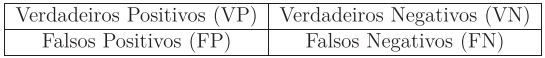
\includegraphics[scale=0.80]{Figuras/Exemplo_matriz_de_confusao.png}
	\end{center}
    \legend{Fonte:\cite{Carvalho2014}}
\end{figure}

\par
\textcolor{red}{Segundo \citeonline{Carvalho2014}, a  matriz de confusão funciona da seguinte forma, a tabela acima possui um tamanho 2x2 contendo 2 classes-alvo, onde, ela pode ter 4 valores possíveis que é: a quantidade de instâncias classificadas corretamente para a classe X (Verdadeiros Positivo), a quantidade de instancias da classe X que foram classificadas incorretamente na classe Y (Falso Positivo), a quantidade de instancias da classe Y que foram classificadas corretamente (Verdadeiro Negativo) e a quantidade de instancias da classe Y que foram classificadas incorretamente na classe X (Falso Negativo).}

\par
\textcolor{red}{Podemos notar que a matriz de confusão é uma ótima ferramenta para verificar a acurácia do algoritmo, fornecendo maiores informações da estimativa de erro obtida pela validação cruzada.}

%==========================
% MINERAÇÃO DE DADOS EDUCACIONAIS
%==========================

\section{Mineração de Dados Educacionais}

\par
Há pouco tempo, com o crescimento dos cursos a distância e também com aqueles que usam suporte computacional, muitos cientistas da área de Informática na Educação, têm demonstrado interesse em usar a mineração de dados para solucionar perguntas científica na área da educação \cite{Baker2011}. Nesse contexto, uma nova área de pesquisa surgiu denominada como Mineração de Dados Educacionais (MDE).

\par
A área de MDE (do inglês, \textit{Educational Data Mining}, EDM), é uma área que tem como proposito de desenvolver ou adaptar técnicas e algoritmos de mineração de dados existentes na literatura, de tal modo que sirvam a entender melhor os dados educacionais, gerados principalmente por professores e estudantes, tais como AVAs (Ambiente Virtual de Aprendizagem), STIs (Sistemas de Tutores Inteligentes), entre outros \cite{Costa2012, Marques2014}.

\par
Segundo \citeonline{Coutinho2016}, a MDE tem como apoio de disponibilizar a descoberta de conhecimentos que sejam importantes, único e útil, tais como: identificar padrões entre alunos, analisar o desempenho através de predição e a identificar perfis de forma que auxilie a gestão qualitativa do ensino a distância (EAD). Os trabalhos nessa área, estão bastante concentrados em situações relacionados a um tipo específico de instituição, no caso, as Instituições de Ensino Superior (IES).

\par



% ----------------------------------------------------------
% Revisão de Literatura
% ----------------------------------------------------------
\chapter{TRABALHOS CORRELATOS}
\label{chapter:correlatos}

\par
Neste capítulo serão apresentados alguns trabalhos relacionados com este, que envolvem mineração de dados aplicado na área educacional, com o objetivo de extrair informações contida no banco de dados dos candidatos que prestaram a prova do ENEM ou a prova do vestibular de alguma universidade.

\section{Mineração de Dados Educacionais nos Resultados do ENEM de 2015}

\par
O trabalho de \citeonline{Simon2017} tem como objetivo em gerar um modelo preditivo da base de desempenho médio na área de ciências da natureza e suas tecnologias dos alunos de escolas do ensino médio, baseado nos dados públicos obtidos do Exame Nacional do Ensino Médio (ENEM) de 2015. Tal motivação foi pelo fato do cenário preocupante do baixo desempenho dos alunos do ensino básico no Brasil, conforme os dados de 2015 do PISA (\textit{Programme for International Students Assessment}).

\par
Segundo \citeonline{Simon2017} foi feito o pré-processamento dos dados do ENEM fornecidos pelo INEP, sendo que para cada área avaliada apresentavam-se 25 colunas que representavam uma informação ou variável, onde cada uma delas eram divididas em três categorias: características da escola, indicadores e desempenho. Das 25 variáveis, apenas 9 foram selecionadas como importante para a mineração de dados conforme o indicador da coluna Id representado na Figura 16. 

\begin{figure}[!htp]
	\begin{center}
    \caption{\label{fig:waveform_fig} Variáveis disponibilizadas pelo ENEM por escola.}
	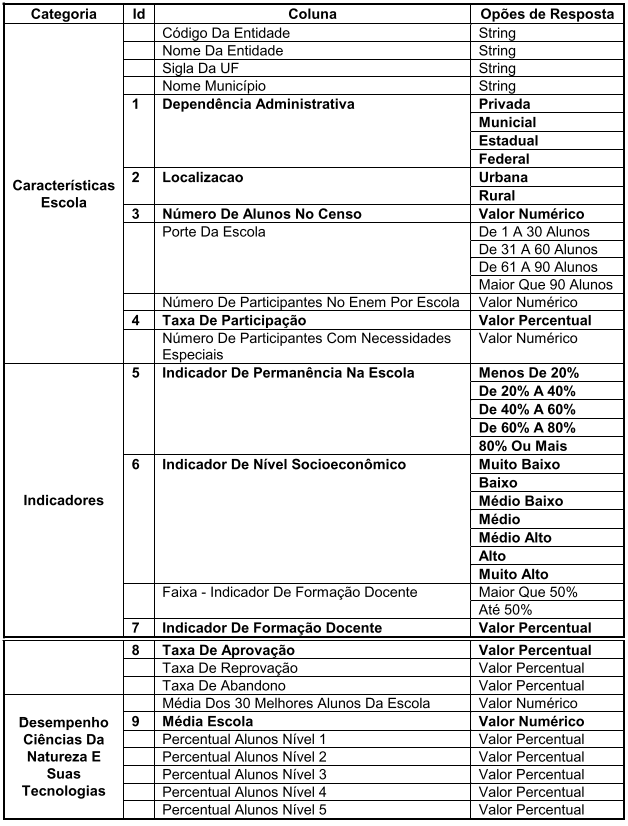
\includegraphics[scale=0.99]{Figuras/Tabela_ENEM.png}
	\end{center}
    \legend{Fonte:\cite{Simon2017}}
\end{figure}

\par
\citeonline{Simon2017} destacaram que a variável Média Escola indicava o desempenho médio dos alunos da escola na área de ciências da natureza e suas tecnologias, onde esses dados eram fornecidos como valor numérico pelo INEP, então para facilitar a mineração dos dados, ele teve que converte-lo para uma categoria mais limitada que foi dividida em quatro valores possíveis, segundo a escala prevista pelo INEP conforme a Figura 17. Os dados fornecidos pelo INEP, vinham em uma planilha no formato .xlsx e teve que ser convertido para .csv, pois, o formato não era suportado pelo software WEKA.


\begin{figure}[!htp]
	\begin{center}
    \caption{\label{fig:waveform_fig} Categoria para os valores Média Escola.}
	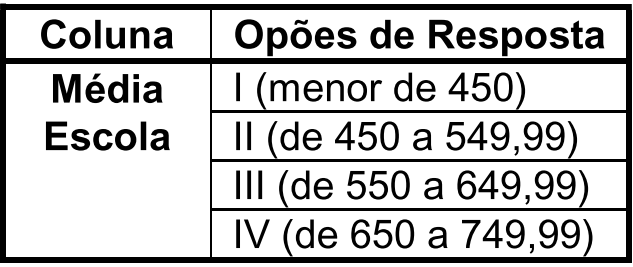
\includegraphics[scale=0.50]{Figuras/Tabela_ENEM_2.png}
	\end{center}
    \legend{Fonte:\cite{Simon2017}}
\end{figure}

\par
Relacionando os fatores socioeconômicos e o índice de desempenho médio em ciências da natureza e suas tecnologias dos alunos, \citeonline{Simon2017} construiu um modelo preditivo utilizando a técnica de mineração de árvore de decisão. Tal técnica, usou o algoritmo j48 através do software WEKA, que foi executado utilizando a opção de \textit{cross-validation}, onde o valor para \textit{fold} era igual a 10 e com a variável dependente Média Escola. Com a árvore obtida, demonstrou como variável independente mais relevante foi a variável Tipo Escola, que se divide entre quatro valores: privada, federal, estadual e municipal.

%Variavel dependete seria o resultado e a variavel independente seria o caminho que ele iria percorre até o resultado. Exemplo: variavel dependete (aluno passou | aluno não passou), variavél independente(entregou os trabalhos, participou das aulas, tirou nota boa na prova, numeros de faltas e etc).

\par
Depois da variável Tipo Escola, a variável hierarquicamente seguinte é a Nível socioeconômico e a partir dela as variáveis seguintes se alternam de posição conforme as funções dos valores dos níveis superiores. Como resultado, sobre o desempenho médio dos alunos na área de ciências da natureza e suas tecnologias, as categorias que mais se destacaram foram a III e IV, acima de 550 pontos, que ocorreram nas escolas: privadas e estaduais com o nível socioeconômico muito alto, federais com o nível médio alto e muito alto e municipal com o nível médio alto.

\par
Em comparação com o trabalho proposto neste TCC,  a base de dados dos fatores socioeconômico e outras informações fornecidos do ENEM pelo INEP, que está relacionado na parte de pré-processamento, é semelhante aos dados fornecidos pela Comissão Permanente do Vestibular (CPV) da UFRR, como base pretende-se adotar as mesmas variáveis que foram escolhidas no trabalho de \citeonline{Simon2017} para agilizar o processo de minerar os dados mais importante para solucionar o problema que é apresentado neste trabalho.

\par
Outro ponto importante é o modelo preditivo que foi abordado, que é a técnica de mineração de Árvore de Decisão que utiliza o algoritmo J48 do software WEKA, já que neste trabalho será utilizado um conceito parecido, contudo será usado um modelo de classificação, outro ponto, seria de utilizar a opção de \textit{cross-validation}, no caso o K-\textit{folds}, que foi usado no trabalho de \citeonline{Simon2017} para os treinos e testes dos dados para a validação do modelo.



\section{Prática de Mineração de Dados no Exame Nacional do Ensino Médio}

\par
O trabalho de \citeonline{Silva2014}, apresenta um estudo de mineração de dados educacionais, mais especificamente, utilizando a tarefa de Associação de Dados de MD no intuito de encontrar padrões de regras nos dados dos questionários socioeconômicos e resultados das provas do Exame Nacional de Ensino Médio (ENEM), fornecidos pelo INEP. O objetivo é de executar as etapas do KDD para o processamento dos dados do ENEM, de modo que por consequência, se utilize a técnica de associação para se encontrar regras proposicionais que relacionam os fatores socioeconômicos do candidato com o seu desempenho na prova.

\par
Para o trabalho de \citeonline{Silva2014}, foi utilizado o banco de dados com os questionários socioeconômico e os desempenhos da prova do ENEM de 2010, fornecido pelo INEP, onde, para acessar os dados do banco dele, foi usado os softwares Oracle Express Edition 11g e PL/SQL Developer que permitem a extração dos dados que foram determinado para o foco da pesquisa. Os dados utilizados para fazer a mineração de dados, foi da região Sudeste das suas capitais: Vitória, Belo Horizonte, São Paulo e Rio de Janeiro.

\par
Na parte de pré-processamento, foi selecionado somente os dados das capitais do Sudeste que resultaram em 452.710 alunos, que entretanto, foram eliminados 310.000 alunos das quatros capitais, pois, eles não compareceram no dia da prova. As questões selecionadas para a pesquisa  foram de quantas pessoas moravam com o candidato, a renda familiar mensal, o nível de escolaridade da mãe e o tipo de escola que cursou no ensino médio. Sendo que essas questões foram analisadas para saber se contribuía, interferia ou afetava a nota e o desempenho do candidato na prova.

\par
Baseado nas respostas das questões analisadas, a nota da prova objetiva foi classificada conforme o conceito mostrada na Figura 18. %Para a preparação da regra de associação, \citeonline{Silva2014} fez uma limpeza e integração nos dados, alterando as colunas principais para binominais, quer dizer, em 0 e 1, sendo 1 a opção que foi respondida no questionário e 0 para o restante das opções que não foi escolhida no mesmo questionário, isso aplica também a categoria da prova, como podemos ver representado na Figura 14, onde o aluno não foi inserido sendo três de quatro delas. 


\begin{figure}[!htp]
	\begin{center}
    \caption{\label{fig:waveform_fig} Relação de tranformação da nota em conceito.}
	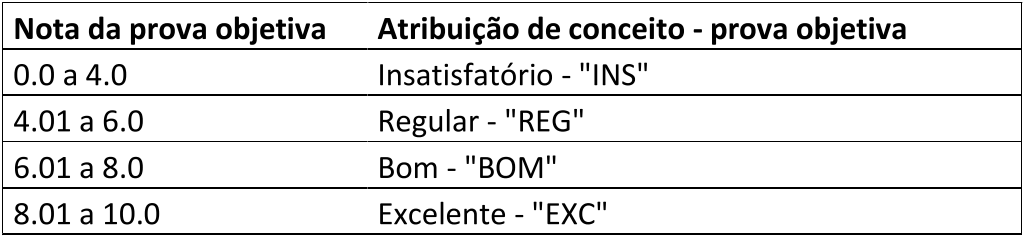
\includegraphics[scale=0.50]{Figuras/Prova_objetiva.png}
	\end{center}
    \legend{Fonte:\cite{Silva2014}}
\end{figure}

%\begin{figure}[!htp]
%	\begin{center}
%    \caption{\label{fig:waveform_fig} Amostragem de alguns dos dados limpos e integrados.}
%	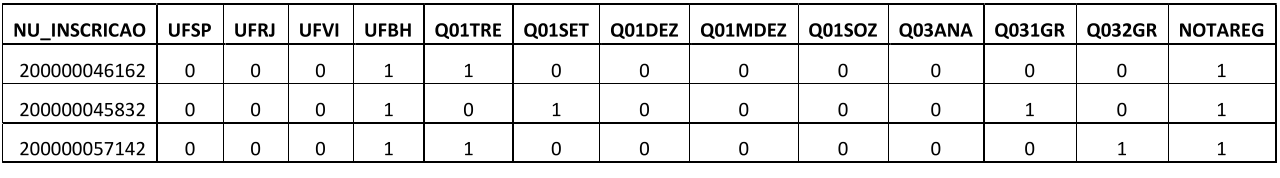
\includegraphics[scale=0.49]{Figuras/Dados_limpos_integrados.png}
%	\end{center}
%    \legend{Fonte:\cite{Silva2014}}
%\end{figure}

%\par
%Observando a segunda linha da Figura 14, percebemos que o candidato é da cidade de Belo Horizonte, mora no total de sete pessoas contando com ele, a mãe dele possui o 1º grau de nível de escolaridade e que a classificação da nota da prova objetiva dele é regular. Para o melhor entendimento, \citeonline{Silva2014} especifica os critérios das colunas, que são:

%\begin{itemize}
%    \item \textbf{NU\_INSCRICAO:} O número de identificação do candidato. 
%    \item \textbf{UFXX:} A sigla da cidade onde o candidato mora.
%    \item \textbf{QXXABC:} Sendo XX a questão escolhida de acordo com o questionário socioeconômico, ABC representa alternativa escolhida da questão de forma abreviada.
%    \item \textbf{NOTAXXX:} Sendo XXX a classificação da nota da prova que o candidato conseguiu. 
%\end{itemize}

\par
Para os experimentos que foram feitos, \citeonline{Silva2014} utilizou o software RapidMiner 5.1 que usa o código aberto Java, e para a tarefa de associação de dados, é usado o algoritmo apriori que na etapa de verificação de itens conjuntos ele faz um processo interativo para a combinação de itens. Este algoritmo realiza busca por largura e é definido em três características: suporte mínimo, confiança mínima e K-itemset.

\par
Dentre as 4 simulações, a regra com maior confiança obtida em cada uma delas, se analisou o seguinte: na simulação 1, se aluno tirou nota regular na prova então ele é de escola pública (80\% de confiança, ocorre 53\% dos alunos), na simulação 2 se os pais tivessem escolaridade de até o primeiro grau então ele era de escola pública (89\% de confiança, ocorre 36\% dos alunos), na simulação 3 se o candidato é de escola pública e possui pais com escolaridade de até o 1º grau, então sua nota da prova é regular (90\% de confiança, ocorre 28\% dos alunos) e na simulação 4 se a nota do candidato é regular, possuir a renda familiar de três salários mínimos e a escolaridade dos pais for de até o 1º, então ele é de escola pública (92\% de confiança, ocorre com 19\% dos alunos).  

\par
Fazendo todos os testes, \citeonline{Silva2014} observou que a medida que o suporte e a confiança diminuía, o número de regras aumentava, como é representado conforme a Figura 19.
 
\begin{figure}[!htp]
	\begin{center}
    \caption{\label{fig:waveform_fig} Simulação de Suporte e Confiança.}
	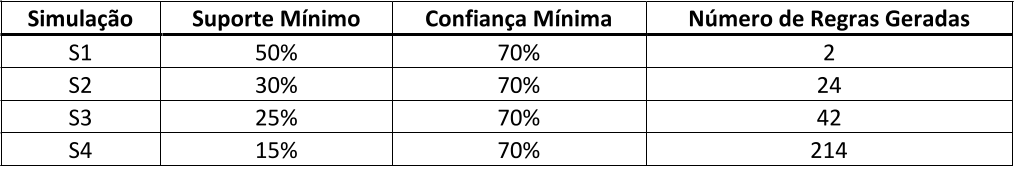
\includegraphics[scale=0.49]{Figuras/Simulacao_suporte_confianca.png}
	\end{center}
    \legend{Fonte:\cite{Silva2014}}
\end{figure}

%\par
%Das quatros simulações, em cada uma se analisou o seguinte: na simulação 1, a regra aplicada era se o aluno era de escola publica então a sua nota prova seria regular (76\% de confiança, ocorre 53\% dos alunos) e a outra regra se o aluno tirou nota regular na prova então ele é de escola pública (80\% de confiança, ocorre 53\% dos alunos). Na simulação 2 a primeira regra com confiança mais baixa gerada era se o candidato morasse com quatro e sete pessoas então ele era de escola pública (74\% de confiança, ocorre 31\% dos alunos) e a última regra com maior confiança era se os pais tivessem escolaridade de até o primeiro grau então ele era de escola pública (89\% de confiança, ocorre 36\% dos alunos).

%\par
%Na simulação 3, a primeira regra gerada de menor confiança é se os pais tivessem escolaridade de até o 1º grau então o candidato é de escola pública e a nota da prova é regular (71\% de confiança, ocorre 28\% dos alunos), e a última regra com maior confiança e se o candidato é de escola pública e possui pais com escolaridade de até o 1º grau, então sua nota da prova é regular (90\% de confiança, ocorre 19\% dos alunos). Na simulação 4, \citeonline{Silva2014} observou que alguns atributos como escolaridade dos pais (2GR) e a renda familiar levava (TRE) o candidato a obter uma nota regular (REG) ou vim de uma escola pública (PUB), como podemos perceber na última regra com maior confiança na Figura 16.

% Podemos evidenciar na penúltima regra que, se o aluno tirou nota regular na prova, os pais tiveram escolaridade até o primeiro grau e a renda da família for de um a três salários mínimos então o aluno estudou em escola pública com 92% de confiança, ocorrendo em 19% dos alunos

%\begin{figure}[!htp]
%	\begin{center}
%    \caption{\label{fig:waveform_fig} Simulação 4, Suporte Mínimo 25\% e Confiança Mínima 70\%.}
%	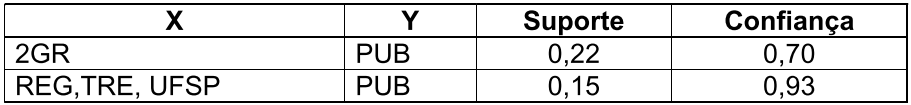
\includegraphics[scale=0.49]{Figuras/Simulacao_quatro.png}
%	\end{center}
%    \legend{Fonte:\cite{Silva2014}}
%\end{figure}

\par
Como representado na Figura 19, \citeonline{Silva2014} verificou que ao diminuir o valor do suporte mínimo, há um acréscimo em casos encontrados na base de dados que utiliza associação de dados, em que se tem regras mais verdadeiras, chegando pelo menos a 90\% de confiança, que são geradas na simulação correspondentes. Para a demonstração, \citeonline{Silva2014} criou faixas de confianças que começava a partir de 70\%, onde, cada faixa era verificada entre as simulações com a quantidade de regras que eram geradas, como por exemplo, na simulação 1, dentre as duas regras, se tinha de 76\% e 81\% de confiança, então ele se enquadra na faixa de 70\% até 80\%, totalizando 50\%.

\begin{figure}[!htp]
	\begin{center}
    \caption{\label{fig:waveform_fig} Sintetização das simulações.}
	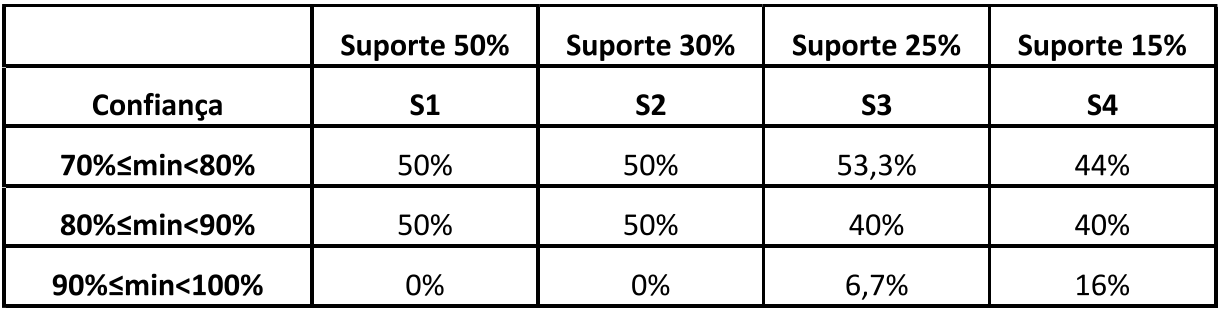
\includegraphics[scale=0.49]{Figuras/Sintetizacao_simulacoes.png}
	\end{center}
    \legend{Fonte:\cite{Silva2014}}
\end{figure}

\par
Contudo, nas regras de maior confiança obtidos com base nas duas últimas simulações, \citeonline{Silva2014} verificou que candidatos de São Paulo que moram com quatro a sete pessoas, com renda familiar de até três salários mínimos, com pais de escolaridade de até 1º grau e com a nota regular obtida no ENEM, então ele é de escola pública, o que reforça que a educação das escolas públicas das capitais da região sudeste está em um nível baixo. Então \citeonline{Silva2014} conclui que com o conhecimento obtido a partir dos resultados, como alta quantidade de pessoas que moram com o candidato, baixa renda familiar e pais com escolaridade de nível primário, são atributos que afetam o baixo desempenho do candidato. 

No trabalho de \citeonline{Silva2014}, demonstra casos semelhantes que pode ocorrer no trabalho proposto, como por exemplo, utilizar dados obtidos do questionário socioeconômico pelo INEP (que neste caso será pelo CPV), para poder relacionar qual destas questões é um dos motivos que afetam o desempenho do candidato na prova, outro ponto, é a eliminação de ruído de dados na parte de pré-processamento, já que nem todos os candidatos inscritos para o vestibular, por algum motivo, não comparecerão para fazer a prova, então será necessário tirar os candidatos que não participaram.

\par
O algoritmo que \citeonline{Silva2014} utilizou para a mineração de dados foi o apriori, que faz uma verificação dos dados através de um processo interativo para combina-los, para então se obter um resultado. Como observado, poderia utilizar como exemplo as técnicas, algoritmo e as questões escolhidas do questionário socioeconômico abordados pelo \citeonline{Silva2014} em conjunto com as outras técnicas e outros conceitos apresentado neste trabalho, para poder assim, obter mais exatidão e aprimoramento nos resultados obtidos.

\par
Um possível problema que encontraria, caso fosse se basear nos exemplos de \citeonline{Silva2014}, é que as questões do questionário socioeconômico fornecidas pelo INEP vem com alternativas de escolha para os candidatos responderem, o que é diferente das questões fornecido pelo CPV, apenas algumas delas vem com alternativa as outras questões vem com resposta direta, um exemplo de uma das questões do questionário socioecômomico do ENEM, é a questão sobre a quantidade de pessoas que moram com o candidatos, onde se tem as seguintes alternativas: (a) três pessoas, (b) quatro pessoas, (c) sete pessoas e (d) mais de sete pessoas.

\section{Descoberta de Conhecimento Sobre o Processo Seletivo da UFPR}

\par
O trabalho de \citeonline{Martinhago2005}, tem como objetivo geral de traçar o perfil dos candidatos ao processo de seleção para a admissão no ensino superior da Universidade Federal do Paraná (UFPR) do campus de Curitiba, utilizando a técnica de mineração de dados Árvore de Decisão através dos algoritmos de classificação J48.J48 e J48.PART, implementados pelo software WEKA. \citeonline{Martinhago2005} utilizou a base de dados dos questionários sócio educacional realizado durante a inscrição do vestibular feito em 2003, os dados do cadastro geral e os dados das notas obtidas na prova e redação, em conjunto com a nota, média das notas e os status (resultado do vestibular) do candidato pelo ENEM. 

\par
Na fase de Pré-processamento, na parte de seleção de dados, \citeonline{Martinhago2005} juntou os 31 itens do questionário sócio educacional com os 24 itens do cadastro geral, para formar uma planilha com base de dados de 55 itens (atributos), para servir como base referencial para aplicação das técnicas de mineração. Ao analisar a base de dados, foi detectado inúmeros itens de dados em branco, valores absurdos ou erro de digitação, logo, \citeonline{Martinhago2005} teve que preencher esses dados com a letra N (NULL), pois, a ferramenta WEKA que foi utilizado, necessita que todos os registros estejam preenchidos. Também foi eliminado atributos que eram repetidos por causa da junção das duas planilha e dados que eram irrelevantes para a pesquisa, tais como protocolo, bairro, CEP e etc.

\par
Na fase de Mineração de Dados, \citeonline{Martinhago2005} utilizou a ténica de classificação de mineração, a Árvore de decisão, utilizando o algoritmo J48 através do software WEKA, para a criação do modelo preditivo aplicado na base de dados obtidos de 46.532 candidatos. No momento, foram realizados testes onde foi selecionado alguns atributos, tais como, idade, sexo, notas e etc., nos testes seguinte, foi utilizado os mesmos atributos dos testes anteriores em conjunto com alguns atributos culturais e sócio educacional, tais como, o turno cursado (se fez cursinho ou não), o tipo de escola e etc. Sucessivamente, foram realizados outros testes com outros atributos.

\par
Utilizando o algoritmo J48, em cada execução, várias regras foram geradas e o resultados obtidos para cada base de dados analisados foi o seguinte: para a base de dados dos candidatos ao 11 cursos mais concorridos, \citeonline{Martinhago2005} observou que o conjuntos de notas categorizados com valores acima da faixa de 5 pontos, influenciam na aprovação do candidato, principalmente as notas de redação e língua portuguesa e outras em geral, outra regra relevante, foi de candidatos com notas na faixa de 6 pontos (4,208 a 8,969 pontos) ou acima no ENEM, alcançaram sucesso do vestibular, um exemplo, candidatos para o curso de Direito que obtém nota em Química, Biologia e Matemática acima da faixa de 5 pontos (4,91 a 9,80), segundo \citeonline{Martinhago2005} geralmente tem chance de ser classificado após a análise da redação.

\par
Para o curso mais concorrido, que no caso foi Medicina, segundo \citeonline{Martinhago2005} as notas obtidas nas provas do vestibular e o do ENEM, foi o principal fator que influenciou na aprovação do candidato ao contrário dos fatores sócioeconômico e culturais, que não foram considerados relevantes nos testes realizados, sendo que nas pesquisas do INEP, fatores como renda familiar, escolaridade dos pais, ter feito cursos de pré-vestibular e ter estudado em escola particular ou pública, seriam determinantes para influenciar a aprovação do candidato no vestibular para o curso de Medicina, porém, mesmo não sendo os principais fatores que influenciam, ainda sim as condições sócioeconômicas interferem na aprovação desse curso. 

\par
Para a base de dados dos candidatos aos onze cursos menos concorridos, através das regras geradas nos testes, segundo \citeonline{Martinhago2005} a notas que influenciaram na aprovação dos candidatos foi em Geografia, Redação, Língua Estrangeira e História e as notas que não foram importantes para aprovação eram Matemática, Química e Física. \citeonline{Martinhago2005} percebeu que uma das regras mais importante como a escolaridade dos pais, influenciavam na aprovação. Alguns dos fatores interessantes que foram extraídos é de que nos cursos menos concorridos os candidatos que foram aprovados, tinham concluído o Ensino Médio a mais de 5 anos e que vinham de escolas públicas ao contrário dos cursos mais concorridos onde essa relação não era frequente, outro fator, é de o candidato ter ou não feito cursinho, não influenciava no resultado.

\par
Para a base de dados contendo os dados de todos os candidatos ao vestibular, \citeonline{Martinhago2005} notou que para as regras geradas, a maioria dos candidatos moram com os pais, não trabalham e que estão em uma faixa de 17 a 20 anos. Observou também, que as pontuações obtidas pelos candidatos para um curso onde na área dele a nota de algumas disciplinas são essenciais para o vestibular, não tem tanta influência no resultado como a pontuação obtida em outras disciplinas de outras áreas, por exemplo na área de exatas, como o curso de Estatística onde as notas de Geografia, Língua estrangeira e História influenciam na aprovação do candidato, ao contrário da área de humanas como Ciências Sociais, onde notas como Matemática, Física e Química, influenciam nos resultados de aprovação. 

\par
Assim como os trabalhos anteriores que são semelhantes a este TCC proposto, o trabalho de \citeonline{Martinhago2005} usa como base de dados para o seus experimentos os dados dos questionários socioeconômico e os dados do cadastro geral dos candidatos do vestibular da UFPR para o seus testes de mineração, a diferença é que \citeonline{Martinhago2005} fez junção com alguns dados fornecidos pelo ENEM para produzir mais regras e ter um melhor resultado na sua classificação. Outro fator semelhante é que é utilizado a técnica de mineração a Árvore de Decisão usando o algoritmo J48 pela ferramenta WEKA para a geração de regras para se obter os resultados. Assim como \citeonline{Martinhago2005} encontrou alguns dados em branco e atributos repetidos e teve que adaptar para o software WEKA, presumo que neste trabalho os mesmos problemas durante a seleção e pré-processamento de dados serão encontrados.

%==========================================================
% REVISÃO SISTEMÁTICA
%==========================================================
\section{Síntese dos Trabalhos Correlatos}

\par
Foram analisados na literatura, trabalhos que discorrem sobre a utilização de mineração de dados em uma base de dados de um vestibular, para a criação de um modelo de classificação ou predição através de regras criadas, a fim de gerar perfis dos candidatos que são aprovados ou saber quais foram os fatores que afetaram ou contribuíram no desempenho do candidato na sua nota da prova.

\par
Em \citeonline{Simon2017}, motivados pelos problemas de infraestrutura apresentados pelo Censo Escolar da Educação Básica de 2016, criaram um modelo preditivo que relacionava o perfil socioeconômico dos candidatos fornecidos pelo INEP com a infraestrutura das escolas apresentados pelo PISA para associar ao desempenho dos alunos em exames, no caso, a prova do ENEM.

\par
\citeonline{Silva2014}, em suas pesquisas identificaram fatores que diminuem o desempenho dos candidatos, através da técnica de mineração baseada em regras de associação que utilizavam diferentes parametrizações do algoritmo apriori. Dados esses utilizados dos questionários socioeconômicos preenchidos pelos candidatos na edição de 2010 do ENEM da região Sudeste. Essas informações, especificamente as respostas de quatro perguntas, são relacionadas com o resultado de desempenho desses alunos.

\par
Por fim, \citeonline{Martinhago2005} investigou a base de dados sobre os vestibulandos da UFPR de 2003, como os dados dos questionários socioeconômico preenchidos pelos candidatos durante as inscrições, os dados do cadastro geral que contém as notas obtidas da prova e redação e o resultado do vestibular em conjunto com as notas e média das notas obtidas pelo ENEM, para poder traçar o perfil dos vestibulandos, utilizando a técnica de mineração árvore de decisão.

\par
A Tabela 3 visa prestar uma breve comparação entre as características chaves dos trabalhos relacionados e as propostas deste trabalho.

\begin{table}[h!]
\caption{Comparação entre os trabalhos correlacionados e a proposta deste trabalho.}
\centering
\begin{tabular}{c c c c c c c}
\hline \vspace{0.1cm}
      & PAB & EF & WE & TC & CT & TA \\ \hline 
    \vspace{0.1cm} \citeonline{Simon2017} & X & X & X &  &  & X \\ 
    \vspace{0.1cm} \citeonline{Silva2014} & X & X &   & X &  & X \\
    \vspace{0.1cm} \citeonline{Martinhago2005} & X &   & X & X &  &  \\
    \vspace{0.1cm} Este Trabalho & X & X & X & X & X & X \\ \hline 
\end{tabular}
\end{table}


\begin{itemize}
%\item \textbf{Q1:} Quais são os métodos para verificação de circuitos lógicos descritos na linguagem de programação VHDL?
	%\begin{itemize}
	\item \textbf{PAB:} Pré-processamento e análise do banco de dados.
	\item \textbf{EF:} Extração das \textit{features}.
	\item \textbf{WE:} Utilização da ferramenta WEKA para a extração de dados.
	\item \textbf{TC:} Utilização de técnicas de mineração de dados para gerar um modelo de classificação.
	\item \textbf{CT:} Comparativo entre as técnicas de mineração para saber qual foi a mais eficiente.
	\item \textbf{TA:} Utilização de técnicas para avaliar os resultados obtidos.
	%\end{itemize}
\end{itemize}






%1.Pré-processamento e analise da base de dados dos candidatos.
%2.Adotar um algoritmo de aprendizagem de máquina para identificar os fatores que influên-ciam o desempenho dos candidatos.
%3.Definir e aplicar uma técnica de associação de dados, para consolidar os dados dos fatoresde desempenho dos candidatos.
%4.  Definir métodos e técnicas para validar os resultados obtidos.




% ----------------------------------------------------------
% Detalhes de Desenvolvimento do Projeto
% ----------------------------------------------------------
\chapter{MÉTODO PROPOSTO}
\label{chapter:metodo}

\par
Com a grande quantidade de dados que são armazenados pelas universidades de seus candidatos ao vestibular, muitas delas não sabem em como utilizar esses dados para benefício próprio. Com base nesses dados armazenados, especificamente os dados dos candidatos que prestaram o vestibular, se pretende aplicar a mineração de dados educacional, com o objetivo de extrair o conhecimento dessa base para saber quais fatores que afetam o desempenho desse candidato em sua nota do vestibular. Neste contexto o trabalho proposto segue as seguintes etapas para se alcançar esse objetivo conforme a Figura 21.

\par
\begin{figure}[!htp]
	\begin{center}
    \caption{\label{fig:waveform_fig} Diagrama do método proposto.}
	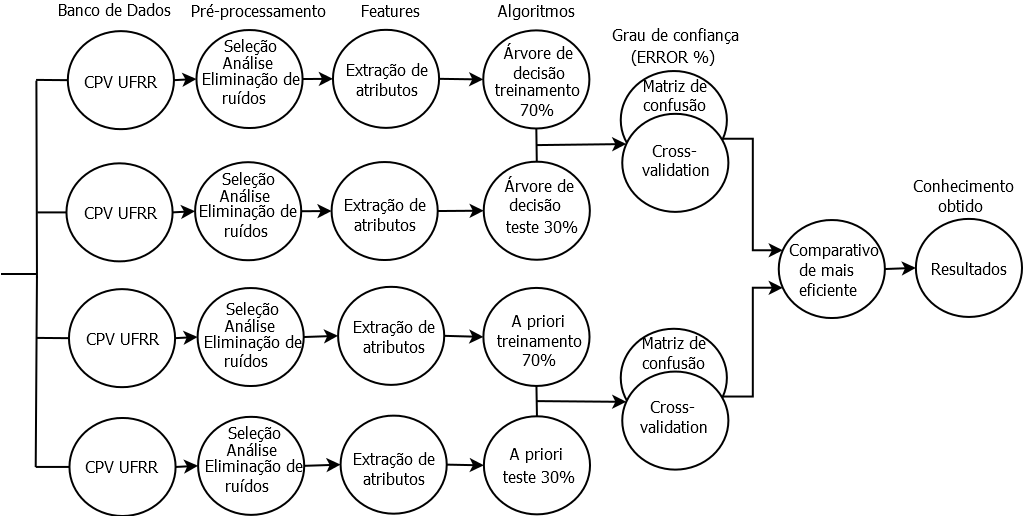
\includegraphics[scale=0.45]{Figuras/Caso_de_uso_metodo_TCC1.png}
	\end{center}
    \legend{Fonte: Próprio autor.}
\end{figure}

\par
Para a fase de pré-processamento (uma das etapas do KDD demonstrado em conceitos de definições), será analisado o banco de dados do vestibular da Universidade Federal de Roraima (UFRR) do ano de 2017 fornecido pela Comissão Permanente de Vestibular (CPV), que está encarregada de gerenciar os dados geral dos candidatos inscritos. Para formar a base de dados onde será aplicado a mineração, estará sendo feita a junção dos dados dos questionários socioeconômico que contém no total de 37 questões e os dados de cadastro geral que são realizados pelos candidatos durante a etapa de inscrição.


\par
Como em todo banco de dados é normal encontrar inconsistência de dados, como ruídos, itens de dados em branco, valores absurdos e erros de digitação, para garantir a qualidade dos dados, serão necessário corrigir esses problemas para que na hora da mineração não ocorra nenhum erro ou que tenha algum resultado incoerente. Tambám será necessário ser feito a eliminação de atributos repetidos assim como dados irrelevantes para a pesquisa e dos dados de candidatos que não compareceram para prestar o vestibular.

\par
Na extração das \textit{features}, pode se ter como base os mesmos atributos que foram selecionados no trabalho de \citeonline{Simon2017}, onde, dentre os 25 atributos apresentados em sua base de dados, depois de alguns testes, apenas 9 delas foram consideradas como relevante para o seu trabalho. Com esses atributos selecionados por \citeonline{Simon2017} será feito um comparativo com as \textit{features} selecionadas pelos algoritmos de seleção de atributos da ferramenta WEKA, para escolher entre elas os atributos mais relevantes que servirão para a mineração e associação de dados deste trabalho.


\par
Depois de selecionar e transformar a base de dados em um formato apropriado, será aplicado a técnica de mineração de árvore de decisão para a análise de dados dos candidatos, a escolha desse método foi pelo seguinte motivo, que segundo \citeonline{Simon2017}, esta técnica serve como um sistema de suporte a decisão, que é utilizado para aprender funções de classificação que mostra o valor de uma variável dependente por meio de dados de variáveis independentes fornecidos. Para alguns autores a técnica de árvore de decisão é considerada uma das abordagens mais poderosas em mineração de dados e descoberta do conhecimento. Contudo, durante o desenvolvimento deste trabalho também serão avaliados outros algoritmos de aprendizagem de máquina, visando assim encontrar uma melhor acurácia do modelo gerado.

\par
Dentre os algoritmos de árvore de decisão, foi optado em utilizar o algoritmo J48, pois, segundo \citeonline{Simon2017} e \citeonline{Martinhago2005} que utilizaram o mesmo algoritmo, o algoritmo J48 gera a árvore de decisão e a transforma em regras de classificação, além de que na literatura é bastante utilizado em aplicações educacionais. O software utilizado para a tarefa de classificação e mineração dos dados é o WEKA que já tem o algoritmo J48 disponível nele, que segundo \citeonline{Simon2017} o WEKA é utilizado a muito tempo em pesquisas que envolvem mineração de dados, sendo aceito amplamente tanto em empresas como academias tendo uma comunidade muito grande que ainda esta ativa.

\par
A ferramenta WEKA foi escolhida pelo motivo de possuir todos os classificadores implementados, além de fornecer outras funcionalidades para pré-processamento, classificação, regressão, agrupamentos, regras de associação, visualização e entre outros \cite{Camilo2009}. Segundo \citeonline{Amaral2016} algumas vantagens de se utilizar o software WEKA é que ela é uma ferramenta gratuita, madura que está disponível desde os anos 90 com inúmeros algoritmos que executam diversas tarefas de aprendizagem de máquina e possui uma interface gráfica interativa, fácil de manusear sem a necessidade de se digitar códigos. 

\par
Para saber a eficiência do algoritmo de árvore de decisão na base de dados proposto, será aplicado a técnica de associação de dados utilizando o algoritmo apriori na mesma base de dados, para saber a eficiência entre as duas através de uma comparação dos seus resultados. Segundo \citeonline{Librelotto2014}, esse algoritmo pode executar várias passagens pelo banco além de trabalhar com um número grande de atributos, tendo como resultado várias alternativas combinadas entre eles através das buscas sucessivas em toda a base de dados. O motivo de se ter essas buscas sucessivas é que ele usa o mesmo raciocínio de dividir para conquistar, com intuito de encontrar regras de associação para todos os atributos possíveis, executando um processo de indução de regras para todas as combinações possíveis de atributos. As regras de associação obtidas são apenas aquelas que o algoritmo classifica como relevante, ou seja, os itens que atendam o suporte mínimo estabelecido. 


\par
Para avaliar os resultados obtidos depois de todos os testes, será utilizado a métrica de avaliação de modelo matriz de confusão e resultados da aplicação \textit{crossvalidation} para determinar se o resultado previsto corresponde ao resultado real. Segundo os trabalhos \citeonline{Simon2017} e \citeonline{Silva2014} que possui base semelhante que será utilizado nesse TCC, nota-se que acurácia resultante para o modelo é aproximadamente a partir de 70\%, ou seja, estaremos utilizando esta porcentagem de acurácia para avaliar os resultados que serão obtidos. Ao final dessas etapas, a partir dos resultados e conhecimento extraído, se espera gerar um perfil para poder encontrar os principais fatores que influencia o bom ou o mau desempenho das notas dos candidatos para o vestibular.

\par 
Através da mineração de dados, com as regras geradas se pode ter como conhecimento relevante para futuras ações da UFRR, referente ao perfil dos candidatos que prestaram seletivo para o vestibular. Como este trabalho tem como intuito uma análise mais profunda dos fatores que afetam o desempenho dos vestibulandos, para poder observar os padrões que tem mais em comum entre eles, pode-se considerar que esta análise está voltada para o desenvolvimento social dos candidatos. Com isso, com os resultados obtidos, pode servir como contribuição para o MEC avaliar em como está indo a sua estratégia do plano de ensino para as escolar públicas, federais e privadas e para o Ministério de Desenvolvimento Social (MDS) para tentar amenizar os possíveis problemas socioeconômico encontrados.



% ----------------------------------------------------------
% Cronograma
% ----------------------------------------------------------
\chapter{PRÉ-PROCESSAMENTO DA BASE DE DADOS}
\label{chapter:projeto}

\par
\textcolor{red}{Nesta sessão será apresentado o processo de modelagem da base de dados que vai ser utilizada para esse projeto, no caso, o pré-processamento dessa base. Será demonstrado o passo a passo da seleção dos dados que são relevantes foram feitos para esta pesquisa, a transformação da base de dados para o formato apropriado para que os algoritmos do software WEKA utilizados, possam usa-las sem que seus resultados obtidos apresentem algum tipo de incoerência.}

\par
\textcolor{red}{Foi mandando um requerimento para a Comissão Permanente de Vestibular (CPV), para que fosse fornecido a base de dados do cadastro e do questionário feitos pelos candidatos que fizeram a prova do vestibular de 2017 para ingressar na universidade no anos de 2018, contudo, a requisição foi negada, pelo fato de que eles não queria expor dados pessoais dos candidatos. Para entrar em om consenso, contornando essa situação, foi fornecido somente os dados do questionário, com a condição de que os Ids dos candidatos fossem trocados por Ids aleatórios, para que as questões não tivessem nenhuma ligação associado aos candidatos.}

\par
\textcolor{red}{No fim, foi obtido através da CPV, somente a base de dados do questionário, contendo uma quantidade de 8.571 registros dos candidatos que o fizeram, durante a inscrição do vestibular da Universidade Federal de Roraima. Com a base de dados obtida, estava pronta para ser feito o pré-processamento dela.}

\section{Pré-processamento}

\par
\textcolor{red}{Com os dados mencionados anteriormente, foram fornecidos no formato de arquivo .xlsx do Excel com uma tabela contendo três colunas de informações com o ID do candidato, a resposta do questionario e o número do questionario atribuido a resposta, como demonstrado na Figura 19. De 37 questões, somente 33 poderam ser fornecidas, pois, quatro delas tinham como respostas dissertativas (que são armazenadas com as outras também, mas como não possuiam um padrão por serem campos abertos, consequentemente, entrava bastante "lixo") e apenas as 33 tinham como resposta opções já fornecidas pelo próprio sitema que eram armazenadas no banco de dados e que davam de ser disponibilizado.}

\par
\textcolor{red}{Para poder começar com a utilização desses dados, foi necessário transformar toda a tabela para um formato apropriado a fim de que os aplicativos do software WEKA os suporte. De início foi feito colunas para cada número do questionário através das funções de filtro e concatenação fornecida pelo Excel, e as linhas abaixo delas seriam as respostas de cada candidato para aquela coluna especifica, como demonstrado na Figura 20. A coluna de ID foi removida já que não era necessário para a mineração, entretanto, ela foi necessária na geração de uma coluna nova rotulada de Aprovado que foi obtida através de duas tabelas contendo informações dos candidatos geral e dos candidatos aprovados.}


\par
\begin{figure}[!htp]
	\begin{center}
    \caption{\label{fig:waveform_fig} Dados fornecidos pela CPV.}
	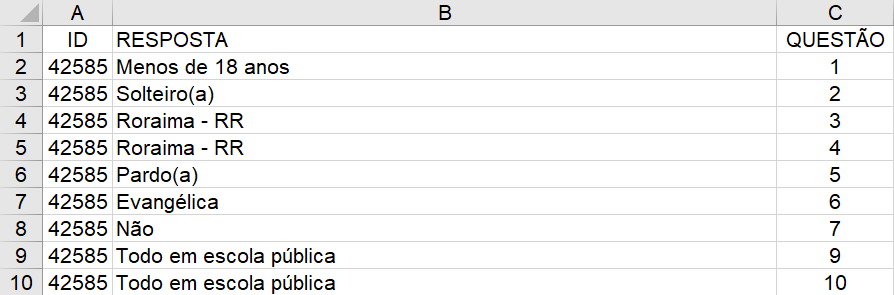
\includegraphics[scale=0.65]{Figuras/Formato_errado.png}
	\end{center}
    \legend{Fonte: Próprio autor.}
\end{figure}

\par
\begin{figure}[!htp]
	\begin{center}
    \caption{\label{fig:waveform_fig} Tabela depois de formatada.}
	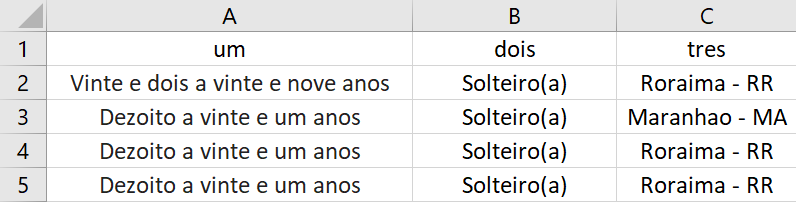
\includegraphics[scale=0.65]{Figuras/Formato_certo.png}
	\end{center}
    \legend{Fonte: Próprio autor.}
\end{figure}

\par
\textcolor{red}{O motivo dessa formatação demonstrado na Figura 20 é que o WEKA identifica a primeira linha como os atributos e as linhas subsequentes os dados relacionados a esses atributos. Como o software trabalha com formato de arquivo próprio denominado \textit{Atribute-Relation File Format} (arff), foi preciso salvar o arquivo que estava no formato xlsx para o formato csv (que separa colunas por ponto e vírgula), pois, o próprio WEKA converte esse tipo de arquivo para o tipo de arquivo que ele trabalha, o arff.}

\par
\textcolor{red}{Também foi necessário se fazer algumas alterações nas informações de dentro da tabela para que depois da conversão não viesse a ocorrer algum erro nos dados. Alterações essas como a remoção de acentos identificados nas informações da tabela, pois, os arquivos no WEKA segundo \citeonline{Amaral2016}, se encontram no formato ASCII que não suportam caracteres acentuados, outra alteração foi a de transformar números para textos, pois, o tipo de dado em cada coluna só pode ser \textit{numeric nominal}, \textit{string} ou \textit{date}, e por fim, a última alteração foi a da remoção de virgulas encontradas nos dados, pois, para converter um arquivo csv no formato arff, o WEKA identifica as virgulas como as colunas que separam os dados.}

\par
\textcolor{red}{A última alteração que precisou ser feita foi da transformação dos ponto e vírgula para somente virgula, pois, o Excel ao transformar um arquivo em xlsx para csv, ele faz com a separação da coluna seja feita por ponto e vírgula o que acaba ocasionando erros e inconsistência nos dados quando o arquivo é convertido do csv para o arff, pois, o WEKA considera o caractere virgula como a representação das colunas que separam os dados. Após ter feito todos esses processos que foram mencionados anteriormente, a conversão do arquivo foi um sucesso, não tendo sido encontrado nenhum problema e inconsistência nos dados que possam ocasionar erro durante o processo de mineração.}


\subsection{Arquivo ARFF}

\par
\textcolor{red}{Após todo o processo de conversão, internamente, o arquivo arff possui duas seções principais: um cabeçalho e uma área de dados. Segundo \citeonline{Amaral2016}, um cabeçalho deve possuir o nome do conjunto de dados através do atributo relação, no caso, o nome do conjunto deve ser acompanhado pela marca @relation seguido com os atributos que compõem a relação com a marca @attribute. Como podemos ver representado na Figura 21 o arquivo utilizado para a mineração de dados, onde a marca @relation traz o nome do conjunto: Vestibulando de 2017. Se tem no total 34 atributos marcados por @relation, sendo todos os atributos do tipo categórico.} 

\par
\begin{figure}[!htp]
	\begin{center}
    \caption{\label{fig:waveform_fig} Cabeçalho do arquivo arff.}
	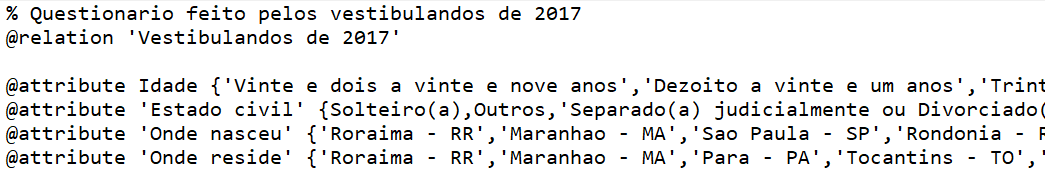
\includegraphics[scale=0.57]{Figuras/arquivo_arff.png}
	\end{center}
    \legend{Fonte: Próprio autor.}
\end{figure}

\par
\textcolor{red}{A seção de área de dados tem o seu início definido pela marca @data, onde os dados dessa área são posicionados em linhas, separados por vírgulas, na mesma ordem em que foram colocados os atributos que teve como um total de 8.571 linhas (que é a quantidade de inscritos que responderam o questionário ), como representado na Figura 22.}

\par
\begin{figure}[!htp]
	\begin{center}
    \caption{\label{fig:waveform_fig} Área de Dados do arquivo arff.}
	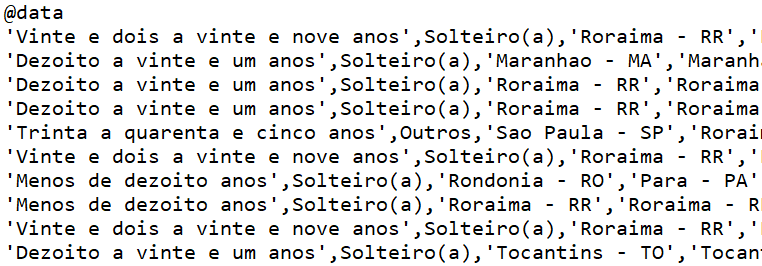
\includegraphics[scale=0.60]{Figuras/arquivo_arff_2.png}
	\end{center}
    \legend{Fonte: Próprio autor.}
\end{figure}


\subsection{Selecionando os Atributos}

\par
\textcolor{red}{Para muitos classificadores, quando recebem uma grande quantidade de atributos, acaba ocasionando um efeito de superajustes nos modelos que os tona ineficiente, segundo \citeonline{Amaral2016}, esse efeito é conhecido como maldição da dimensionalidade. Esse mesmo tipo de problema ocorre com os atributos dos dados socioeconômicos fornecidos para esse trabalho, no caso, para o algoritmo de classificação J48 que é utilizado. Para contornar esse problema foi utilizado a técnica de seleção de atributos que o Explorer do software WEKA disponibiliza, no qual descobre quais atributos são mais relevantes para a melhor generalização do modelo.}

\par
\textcolor{red}{Para a execução da seleção de atributo no WEKA, é preciso selecionar o avaliador de atributo (\textit{Attribute Evaluator}) e o método de busca (\textit{Search Method}). Como demonstrado na Figura 23, o método de avaliação escolhido foi a opção \textit{CfsSubetEval}, onde ele considera a capacidade preditiva individual de cada recurso, diretamente com o grau de redundância entre eles e para o método de busca foi escolhido a opção \textit{GreedyStepwise} que faz uma busca avançada tanto pra frente quanto pra trás através do espaço de subconjuntos de atributos e também pode criar uma lista classificada de atributos, fazendo que sejam registrados na o ordem em que elas foram selecionadas \cite{WEKA}. Além do que, segundo \citeonline{Amaral2016}, esse método de busca é compatível com o algoritmo de avaliação de atributo escolhido. }

\par
\begin{figure}[!htp]
	\begin{center}
    \caption{\label{fig:waveform_fig} Representação do avaliador de atributo e método de busca.}
	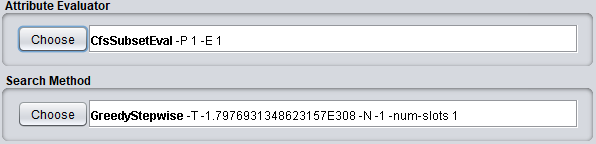
\includegraphics[scale=0.90]{Figuras/Avaliador_de_atributo.png}
	\end{center}
    \legend{Fonte: Próprio autor.}
\end{figure}

\par
\textcolor{red}{Nos primeiros testes de seleção, foi optado de usar tanto a opção de treino para todo o conjunto quanto a opção de \textit{cross-validation} com um número 10 de fold, nos 33 atributos relacionado ao atributo Aprovado, para os dois casos, o atributo mais relevante para a classificação era o estado onde o vestibulando residia como demonstrado na Figura 24. Então, para resolver esse problema, teve que ser feita a remoção de alguns atributos que eram desnecessários para esta pesquisa como o melhor horário para cursar a universidade, o que esperar do curso, como soube do processo seletivo e entre outros, depois de ter feito a remoção, de 33 atributos sobraram somente 22 para serem aplicados no algoritmo de seleção do WEKA.}

\par
\begin{figure}[!htp]
	\begin{center}
    \caption{\label{fig:waveform_fig} Resultado da seleção de atributos utilizando o método cross-validation para o treino.}
	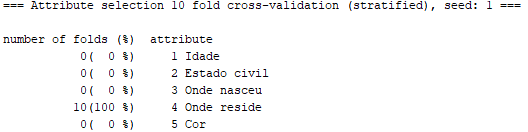
\includegraphics[scale=0.99]{Figuras/33_atributos.png}
	\end{center}
    \legend{Fonte: Próprio autor.}
\end{figure}

\par
\textcolor{red}{}

\par
\textcolor{red}{}



\par
\textcolor{red}{Mas antes de ser aplicado a técnica de seleção, foi feito os seguintes testes, primeiro foi utilizado os atributos para o teste de seleção que os autores dos trabalhos correlatos que teve como base para este projeto. Foi utilizado os 4 atributos mais importantes para a pesquisa que os autores \citeonline{LeandroSilva2014} selecionaram, mais os 9 atributos de 25 que \citeonline{Simon2017} selecionaram, entretanto, apena 2 de 9 atributos foi utilizado para o teste, por que, os outros 7 eram dados de escolas que o INEP fornecia, diferente dos dados que a CPV forneceu. Tambem foram selecionados 12 atributos (que tinham em comum com este trabalho) dos 33 atributos que \citeonline{Martinhago2005} obteve como mais relevante para a pesquisa dele}


\par
\textcolor{red}{Juntando os atributos que os três trabalhos selecionaram, teve no total de 13 atributos como base: a escola que cursou o ensino médio, escolaridade da mãe, renda mensal familiar, quantidade de pessoas que moram com a pessoa, idade do candidato, estado civil, com quem reside, escolaridade do pai, ocupação do pai, ocupação da mãe, idade que começou a trabalhar, frequentou algum cursinho e cor de pele. Aplicando o algoritmo de seleção nesses 13 atributos mais o atributo Aprovados, teve como resultado, que apenas 5 deles relacionado ao atributo Aprovado, estavam acima do 70\%  (mais relevantes para a classificação), como demonstrado na Figura 25.}

\par
\begin{figure}[!htp]
	\begin{center}
    \caption{\label{fig:waveform_fig} Resultado da seleção de atributos dos 13 atributos utilizados relacionado ao atributo Aprovado.}
	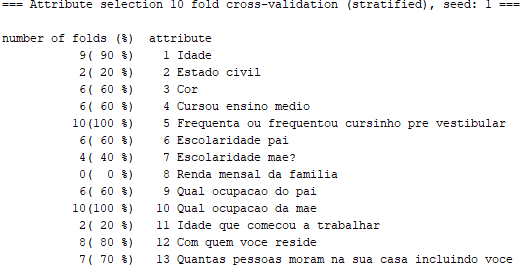
\includegraphics[scale=0.99]{Figuras/13_atributos.png}
	\end{center}
    \legend{Fonte: Próprio autor.}
\end{figure}

\par
\textcolor{red}{Depois do teste que foi feito com os atributos base, foi acrescentado mais um atributo ao teste, para poder mais uma vez executar a seleção de atributos e depois analisar os resultados, isso foi feito sucessivamente até chegar aos 22 atributos. Depois de todo o processo de teste, no final, teve como resultado que os atributos mais relevantes (que ultrapassavam de 70\%) que foram obtidos nos dados fornecidos eram praticamente diferentes dos dados selecionados para o teste base, como demonstrado na Figura 26. O motivo disso é que  como os dados desse projeto possui algumas diferenças com os dados que foram utilizados nos trabalhos correlatos, os atributos que foram selecionados por eles é mais relevantes nos trabalhos dos mesmos do que para esse projeto.}

\par
\begin{figure}[!htp]
	\begin{center}
    \caption{\label{fig:waveform_fig} Resultado dos testes de seleção com o maximo de atributos.}
	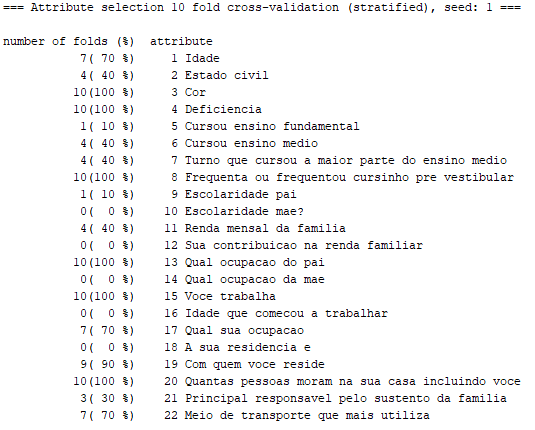
\includegraphics[scale=0.90]{Figuras/22_atributos.png}
	\end{center}
    \legend{Fonte: Próprio autor.}
\end{figure}

\par
\textcolor{red}{}

\par
\textcolor{red}{}

\par
\textcolor{red}{Observando a Figura 26,  os atributos mais relevantes foram: idade do candidato, a cor de pele, se possui alguma deficiência, se frequentou algum cursinho pré-vestibular, ocupação do pai, se o candidato trabalhava, a ocupação do candidato, com quem ele residia, quantidades de pessoas que moram com ele e por último o meio de transporte que ele utiliza. Para ter certeza que os atributos selecionados continuariam com a taxa de relevância acima dos 70\%, foi aplicada a seleção de atributos mais uma vez e o resultados obtidos foi que apenas 8 dos 10 atributos selecionados anteriormente, mantiveram acima dos 70\%, como apresentado na Figura 27.}

\par
\begin{figure}[!htp]
	\begin{center}
    \caption{\label{fig:waveform_fig} Resultado final dos testes de seleção.}
	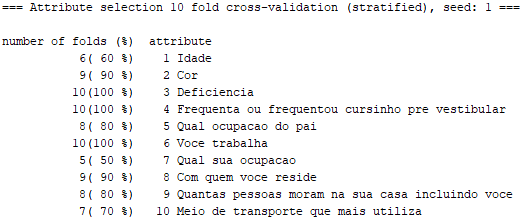
\includegraphics[scale=0.99]{Figuras/10_atributos.png}
	\end{center}
    \legend{Fonte: Próprio autor.}
\end{figure}

\par
\textcolor{red}{Então, os dados que foram obtidos como mais relevantes pela seleção de atributos do Explore do WEKA, que serão utilizados para a classificação, foram: a cor de pele, se possui alguma deficiência, se frequentou algum cursinho pré-vestibular, ocupação do pai, se o candidato trabalhava, com quem ele residia, quantidades de pessoas que moram com ele e por último o meio de transporte que ele utiliza.}

\subsection{Problemas de Classe Rara}

\par
\textcolor{red}{É normal em alguns casos de quando se vai minerar algum dado ocorra o problema de classe rara, que segundo \citeonline{Amaral2016}, explica que quando uma instancia de uma classe é predominante do que outra instancia de outra classe, a consequência é de que o modelo aprenderá somente as características da classe dominante, enquanto ele falhará em classificar novas instancias da outra classe, pelo motivo de ela ser uma classe rara. É o que acontece nos dados desse trabalho, especificamente no atributo de Aprovado que tem no total de 8571 instancias, possuindo a classe Sim com 7784 instancias (81\%) e a Classe Nao com 787 instancias (9\%) como demonstrado na Figura 28.}

\par
\begin{figure}[!htp]
	\begin{center}
    \caption{\label{fig:waveform_fig} Representação do atributo Aprovado com as suas duas classes Sim e Nao.}
	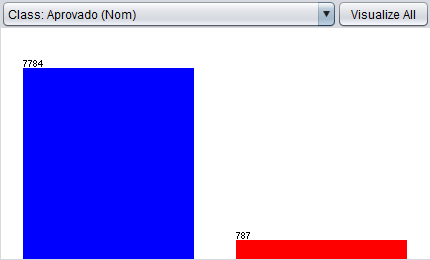
\includegraphics[scale=0.90]{Figuras/Atributo_aprovado.png}
	\end{center}
    \legend{Fonte: Próprio autor.}
\end{figure}

\par
\textcolor{red}{}


\par
\textcolor{red}{Segundo \citeonline{Amaral2016}, a solução mais comum para esse tipo de problema é de utilizar as técnicas de estratificação. No software WEKA, para métodos supervisionado, possui 4 técnicas de estratificação para instancias, no caso, a que foi utilizada para resolver esse tipo de problema foi a técnica SpreadSubsample, pois, segundo o site do software \citeonline{WEKA} esse tipo de filtro gera uma subamostra aleatória de um conjunto de dados, permitindo especificar o \textit{spread} máximo entre a classe mais rara e a classe mais comum, ou seja, balanceado o conjunto de dados dessas duas classe.}

\par
\textcolor{red}{No filtro SpreadSubsample a opção escolhida para a distributionSpread (\textit{spread} máximo distribuição de classe) foi de 1 que representa a opção de distribuição uniforme que é demonstrada na Figura 29. Depois de ser aplicado esse filtro na classe de Aprovado, tem como resultado um conjunto de dados balanceado tanto para a classe mais comum (Sim) como a classe mais rara (Nao), como representada na Figura 30.}

\par
\begin{figure}[!htp]
	\begin{center}
    \caption{\label{fig:waveform_fig} Representação da configuração  do filtro SpreadSubsample.}
	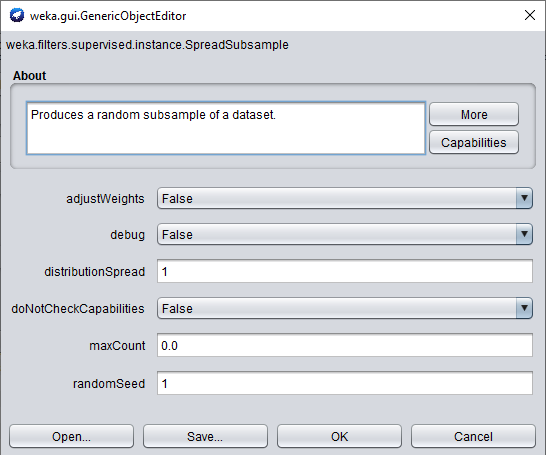
\includegraphics[scale=0.80]{Figuras/SpreadSubsample.png}
	\end{center}
    \legend{Fonte: Próprio autor.}
\end{figure}

\par
\begin{figure}[!htp]
	\begin{center}
    \caption{\label{fig:waveform_fig} Resultado do balanceamento do atributo Aprovado.}
	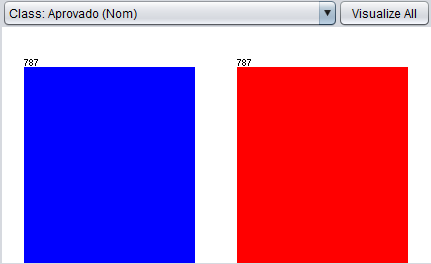
\includegraphics[scale=0.80]{Figuras/Atributo_aprovado_balanceado.png}
	\end{center}
    \legend{Fonte: Próprio autor.}
\end{figure}



% ----------------------------------------------------------
% Cronograma
% ----------------------------------------------------------
\chapter{AVALIAÇÃO EXPERIMENTAL E ANÁLISE}
\label{chapter:Avaliacao}


\section{Testes}

\par
\textcolor{red}{oi.}

\subsection{Árvore de Decisão}

\subsection{Apriori}

\section{Resultados}


% ----------------------------------------------------------

% Cronograma
% ----------------------------------------------------------
\chapter{Resultados}
\label{chapter:Resultados}

\par
\textcolor{red}{Nesta seção serão apresentados os resultados obtidos após as avaliações do modelo, que foi feito com os algoritmos de classificação e associação. Será demonstrado quais variáveis foram classificadas com maior relevância, as ramificações geradas com maior quantidade de registros que percorrem elas, além das regras obtidas para base através do algoritmo de associação.}

\section{Classificação}

\par
\textcolor{red}{Os resultados obtidos com o algoritmo de classificação apresentam um valor mediano de acurácia para o modelo utilizado. A técnica de classificação que foi utilizada, classificou corretamente em torno de 53\% das instâncias que pertence ao conjunto de teste, em relação à classe do resultado que foi obtido. Com base do modelo de árvore de decisão deduzido pelo algoritmo J48, foi possível analisar o grau de interação e a relação das variáveis de acordo com o caminho de interações percorrido pelas respostas do questionário feitas pelos candidatos.}

\par
\textcolor{red}{A árvore obtida apresentou como variável independente principal para a classificação o atributo Deficiencia, que se divide em 5 valores: Nao, Sim visual, Sim outro tipo, Sim fisica e Sim auditiva. As próximas variáveis com maior relevância mudavam de acordo com o valor que era obtido, sendo que, quando a resposta do candidato era de que ele não possuía alguma deficiência ou que ele possuía uma deficiência visual, a variável com maior importância para onde os valores eram direcionados era se ele frequentava ou frequenta cursinho particular, enquanto, para aqueles que possuíam deficiência física ou auditiva eram direcionados para a variável Cor (cor de pele), como apresentada na Figura 39.}

\par
\begin{figure}[!htp]
	\begin{center}
    \caption{\label{fig:waveform_fig} Representação das principais variáveis da árvore de decisão.}
	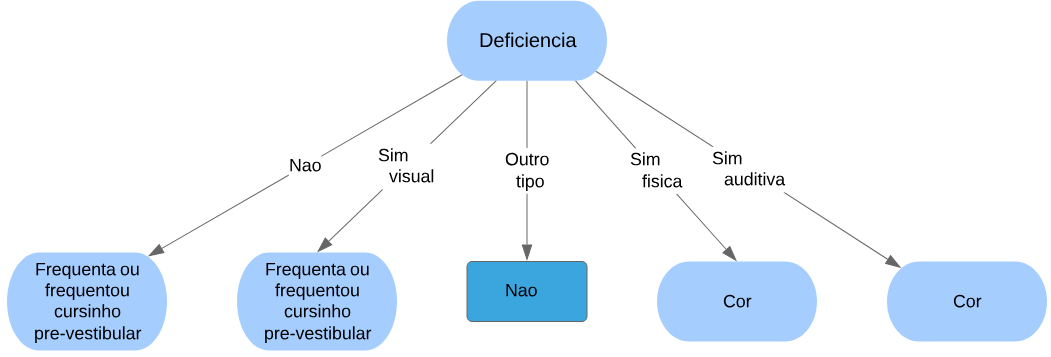
\includegraphics[scale=0.57]{Figuras/Arvore_gerada_grau2.png}
	\end{center}
    \legend{Fonte: Próprio autor.}
\end{figure}


\par
\textcolor{red}{É possível observar na Figura 37, que para os candidatos que responderam que possuíam outro tipo de deficiência, o valor da resposta era direcionado para um nó folha da classe Nao pertencente a variável dependente Aprovado, isto é, os candidatos que possuíam outro tipo de deficiência que não foram mencionados como opção de resposta da questão, não foram capazes de passar no vestibular (um total de 9 candidatos). A partir do terceiro nível de profundidade, para os candidatos que não possuíam nenhum tipo de deficiência a ramificação da árvore se expandia (tracejado pela linha vermelha), enquanto, diferentemente para os candidatos que possuíam algum tipo de deficiência, eles eram direcionados para os nós folhas da variável Aprovado (tracejado pela linha verde), como apresentado na Figura 40.}

\par
\begin{figure}[!htp]
	\begin{center}
    \caption{\label{fig:waveform_fig} Árvore completa.}
	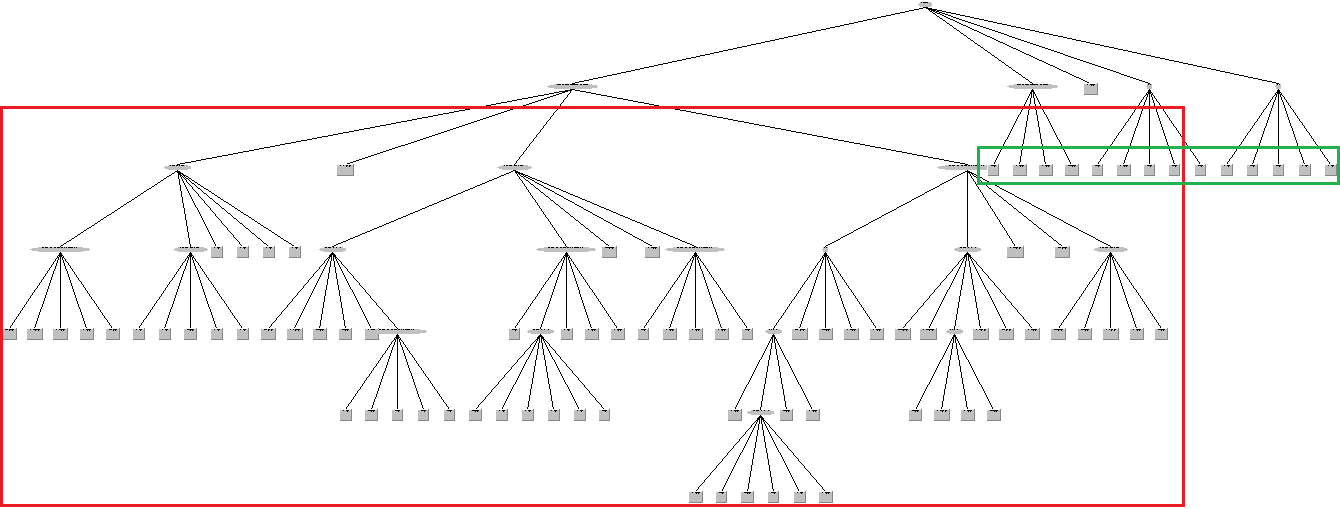
\includegraphics[scale=0.45]{Figuras/Arvore_completa.png}
	\end{center}
    \legend{Fonte: Próprio autor.}
\end{figure}


\subsection{Resultados Obtidos Para os Candidatos que não Possuiam Nenhum Tipo de Deficiência}


\par
\textcolor{red}{Avaliando a árvore que foi gerada, através da maior quantidade de registros que se encaixam pelo caminho percorrido das ramificações até as folhas, foi obtido os seguintes resultados, começando pela ramificação maior que era a dos candidatos que não possuiam nenhum tipo de deficiencia, a variavel com maior relevancia que foi classificada após o variavel independente principal era se o candidato frequentava um cursinho pré-vestibular. Foi classificado que todos aqueles que frequentaram por mais de um ano algum cursinho, não foram aprovados no vestibular.}

\par
\textcolor{red}{Para aqueles que frequentaram o cursinho por um ano, o atributo correspondente seguinte era a quantidade de pessoas que moravam com ele, sendo que, a maior taxa de candidatos aprovados para essa variavel era quando possuia 3 pessoas morando com ele e para reprovados era quando possuia de 4 a 5 pessoas. Já para os candidatos que ficavam por um semestre fazendo o cursinho, a variavel correspondente seguinte era o meio de transporte que ele utilizava, a maior taxa de aprovados era pra aqueles que usavam o transporte coletivo e para os reprovados eram os outros tipos de transportes não eram mencionados como opção de resposta.}

\par
\textcolor{red}{Para aqueles que não frequentavam algum cursinho pré-vestibular, a variável classificada com maior relevância, seguinte, era a quantidade de pessoas que moravam com o candidato, e dependendo dos valores que eram respondidos para essa variável, os atributos em sequência variavam entre cor de pele, ocupação do pai e meio de transporte utilizado. Foi notado que as maiores taxas de aprovados eram para os candidatos pardos, que moravam de 3 a 5 pessoas e que o pai era servidor público, já para aqueles que não foram aprovados, as maiores taxas eram quando o candidato possuía de quatro ou mais pessoas morando com ele, o pai possuía outro tipo de ocupação e o meio de transporte utilizado era o coletivo.}


\subsection{Resultados Obtidos Para os Candidatos que Possuem Algum Tipo de Deficiência}


\par
\textcolor{red}{Diferente dos valores classificados para os candidatos que não possuíam algum tipo de deficiência, para aqueles que possuíam, o nível de profundidade que a ramificação delas alcançou não foi tão grande quanto a outra. Os resultados obtidos foram, primeiro, para os candidatos que eram deficientes visuais, a taxa de maior aprovação na prova era para aqueles que não frequentaram cursinho pré-vestibular, enquanto para aqueles que frequentaram cursinho por mais de um ano a taxa de reprovação era maior.}

\par
\textcolor{red}{Foi possível observar que tanto para os candidatos com deficiência física quanto para auditiva, a variável que mais influenciava para que eles fossem aprovados ou não era cor de pele. Sendo que para os candidatos com deficiência física, aqueles que eram brancos a chance de ser aprovado era maior, diferente para aqueles que eram pardos tendo sua taxa de reprovação muito alta comparada a outros tons de pele.}

\par
\textcolor{red}{Para os candidatos que possuíam deficiência auditiva, aqueles que tinham um tom de pele pardo obtiveram as maiores taxas de aprovação, ao contrário daqueles que possuíam uma cor de pele branca, a taxa de reprovação era alta. Como já foi mencionado anteriormente na parte de avaliação do trabalho, os candidatos que possuíam qualquer outro tipo de deficiência, foram classificados, que nenhum deles tiveram êxito de serem aprovados no vestibular.}


\section{Associação}

\textcolor{red}{Através dos resultados obtidos com o algoritmo de associação, observou que a medida que o suporte mínimo decrescia, a quantidade de regras que eram geradas aumentava. Os resultados das regras geradas foram divididos em duas partes, para os candidatos aprovados e para os candidatos não aprovados.}

%\textcolor{red}{787 registros aprovados, 7784 registros não aprovados, 8571.}


\subsection{Regras Geradas Para os Candidatos Aprovados}

\par
\textcolor{red}{Analisando as regras geradas em cada teste, na Tabela 5 que apresenta a tabela das regras gerada utilizando 22 atributos com 50\% de suporte, são interpretados da seguinte maneira. Para regra com menor transição de itens, diz que se o candidato possui outro tipo de trabalho não mencionado e a sua residência é própria então ele terá chance de ser aprovado com 100\% de confiança. Já para a maior regra gerada, diz que se o candidato não possui alguma deficiência, seu ensino médio é todo em escola pública e possui outro tipo de trabalho não mencionado, então a chance de ele passar é de 100\% de confiança. Para ambas as regras, acontece com 5\% dos candidatos (394 instancias).}


\par
\begin{table}[!htp]
	\begin{center}
    \caption{\label{fig:waveform_fig} Suporte Mínimo 50\% e Confiança Mínima 70\%.}
	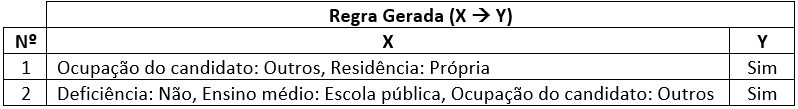
\includegraphics[scale=0.75]{Figuras/Suporte_50_atributos_22.png}
	\end{center}
\end{table}

\par
\textcolor{red}{Para os outros testes com 4 e 9 atributos, com a taxa de 50\% de suporte, nenhuma regra foi gerada para elas. Assim como os resultados do teste de 50\% de suporte, para os testes de 30\% das transições feitas com a quantidade de 4 e 9 atributos, nenhuma regra foi gerada também, já para a base com 22 atributos, foram geradas pelo menos 11 regras no geral, associadas com a variável Aprovados. Sendo que a primeira regra gerada possui 5 itens em sua transição e a última regra gerada chega a possuir 7 itens em sua transição. As regras foram geradas para 236 instancias (3\% dos candidatos), como apresentado na Tabela 6, onde é demonstrado a primeira e a ultima regra gerada.}

\par
\begin{table}[!htp]
	\begin{center}
    \caption{\label{fig:waveform_fig} Suporte Mínimo 30\% e Confiança Mínima 70\%.}
	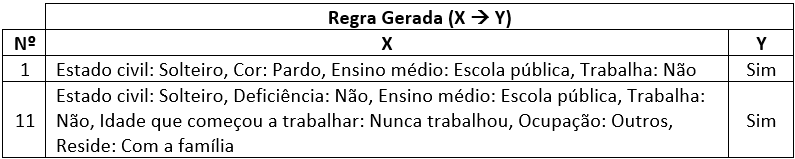
\includegraphics[scale=0.75]{Figuras/Suporte_30_atributos_22.png}
	\end{center}
\end{table}


\par
\textcolor{red}{Avaliando os testes com 25\% de suporte mínimo, foram geradas regras para as bases com 9 e 22 atributos e para a base com 4 atributos nenhuma regra foi obtida. Analisando a única regra que foi gerada para a base com 9 atributos, diz que 2\% dos candidatos que eram aprovados (197 instancias), eles não trabalhavam, não possuíam algum tipo de deficiência e o meio de transporte utilizado era o coletivo, representado na Tabela 7. Já para a primeira regra gerada para a base com 22 atributos, 2\% dos candidatos que foram aprovados (197 instancias) eram solteiros, sustentados pela família e utilizava o transporte coletivo, como representado na Tabela 8.}

\par
\begin{table}[!htp]
	\begin{center}
    \caption{\label{fig:waveform_fig} Suporte Mínimo 25\% e Confiança Mínima 70\% para a base com 9 atributos.}
	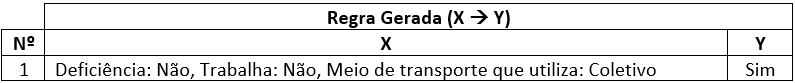
\includegraphics[scale=0.75]{Figuras/Suporte_25_atributos_9.png}
	\end{center}
\end{table}

\par
\begin{table}[!htp]
	\begin{center}
    \caption{\label{fig:waveform_fig} Suporte Mínimo 25\% e Confiança Mínima 70\% para a base com 22 atributos.}
	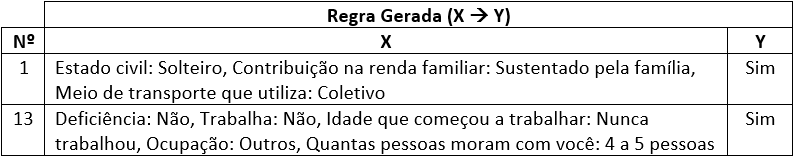
\includegraphics[scale=0.75]{Figuras/Suporte_25_atributos_22.png}
	\end{center}
\end{table}

\par
\textcolor{red}{Com o suporte mínimo de 15\%, as bases de dados com 4 e 9 atributos obtiveram somente uma regra gerada, enquanto, para a base de dados com 22 atributos, foi obtido 67 regras geradas, sendo que é considerada a maior quantidade de regras que já foi gerada para todos os suportes mínimos testados. Começando com a regra gerada para a base com 4 atributos, como demonstrado na Tabela 9, indica que os candidatos que tem uma mãe com ensino médio completo e possui de 4 a 5 pessoas morando com eles, influenciam para que eles sejam aprovados.}

\par
\begin{table}[!htp]
	\begin{center}
    \caption{\label{fig:waveform_fig} Suporte Mínimo 15\% e Confiança Mínima 70\% para a base com 4 atributos.}
	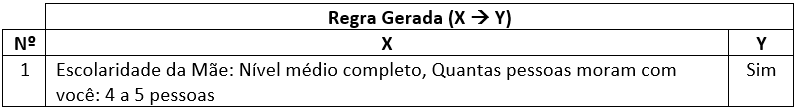
\includegraphics[scale=0.75]{Figuras/Suporte_15_atributos_4.png}
	\end{center}
\end{table}

\par
\textcolor{red}{Já para a base com 9 atributos, a regra gerada indica que os candidatos que possuem um pai que é servidor público, mora com a família e possui de 4 a 5 pessoas morando com eles, são aprovados no vestibular, como apresentado na Tabela 10.}

\par
\begin{table}[!htp]
	\begin{center}
    \caption{\label{fig:waveform_fig} Suporte Mínimo 15\% e Confiança Mínima 70\% para a base com 9 atributos.}
	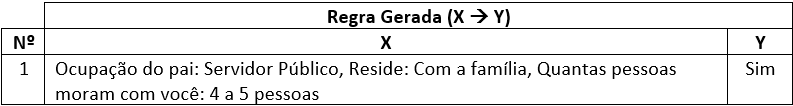
\includegraphics[scale=0.75]{Figuras/Suporte_15_atributos_9.png}
	\end{center}
\end{table}

\par
\textcolor{red}{Para a base de dados com 22 atributos com um suporte mínimo de 15\%, conforme é demonstrado da Tabela 11, na primeira regra gerada, a idade de 18 a 21 anos e a mãe como principal responsável, influenciavam para que o candidato fosse aprovado, enquanto para a última regra gerada, os candidatos que eram pardos, que não frequentavam cursinho pré-vestibular, nunca trabalharam e moravam com a família, eles eram aprovados. As regras geradas paras as bases com 4, 9 e 22 atributos, com um suporte de 15\%, influenciavam 1,4\% dos candidatos (118 instancias).}

\par
\begin{table}[!htp]
	\begin{center}
    \caption{\label{fig:waveform_fig} Suporte Mínimo 15\% e Confiança Mínima 70\% para a base com 22 atributos.}
	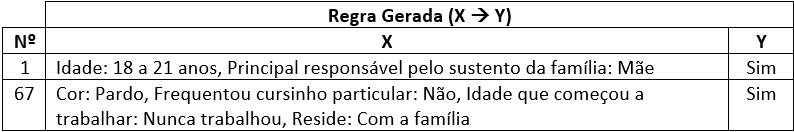
\includegraphics[scale=0.75]{Figuras/Suporte_15_atributos_22.png}
	\end{center}
\end{table}



\subsection{Regras Geradas Para os Candidatos que não Foram Aprovados}


\par
\textcolor{red}{Para os testes com a base de dados dos candidatos que não foram aprovados, dos 4 suportes mínimos utilizados, apenas 3 geraram regras para as bases de dados, que foram os suportes de 30\%, 25\% e 15\%, sendo que para os suportes testados, geraram regras somente para a base com 22 atributos. Começando com o suporte mínimo de 30\%, como podemos ver na Tabela 12, foi gerado apenas uma regra associada a variável de Aprovados, indicando que que 27\% dos candidatos (2.335 instancias) que não foram aprovados eles eram solteiros, com o tom de pele pardo, não trabalhavam e possuíam residência própria.}


\par
\begin{table}[!htp]
	\begin{center}
    \caption{\label{fig:waveform_fig} Suporte Mínimo 30\% e Confiança Mínima 70\% para a base com 22 atributos.}
	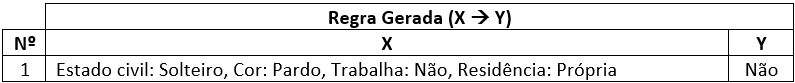
\includegraphics[scale=0.75]{Figuras/Suporte_30_Nao_atributos_22.png}
	\end{center}
\end{table}

\par
\textcolor{red}{Semelhante ao anterior, o suporte mínimo de 25\% gerou uma única regra, somente para a base de 22 atributos, como demonstrado na Tabela 13, a regra gerada indica que 22\% dos candidatos que não foram aprovados (1.946 instancias), eram solteiros, possuem uma renda mensal familiar de 2 a 4 salários mínimos, a residência deles é própria e moram com a família.}

\par
\begin{table}[!htp]
	\begin{center}
    \caption{\label{fig:waveform_fig} Suporte Mínimo 25\% e Confiança Mínima 70\% para a base com 22 atributos.}
	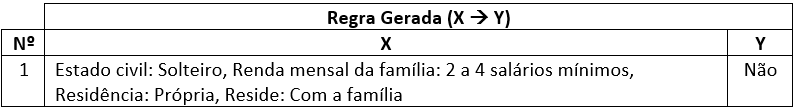
\includegraphics[scale=0.75]{Figuras/Suporte_25_Nao_atributos_22.png}
	\end{center}
\end{table}

\par
\textcolor{red}{Com um suporte mínimo de 15\%, foi obtido regras apenas para a base de dados com 22 atributos, tendo um total de 23 regras geradas. Para a primeira regra, os candidatos que não era deficiente, o ensino médio foi em escola particular e possuía outro tipo de trabalho que não foi mencionado nas opções dadas, eles não eram aprovados. Já para a última regra, para os candidatos com a idade entre 18 a 21 anos, solteiro, não possuía algum tipo de deficiência, o ensino médio foi em escola pública, era sustentado pela família, não trabalhava, possuía uma residência própria e morava com a família, todos esses fatores influenciavam para que eles não fossem aprovados, que era no total de 14\% dos candidatos (1.168 instancias), conforme o que é demonstrado na Tabela 14.}

\par
\begin{table}[!htp]
	\begin{center}
    \caption{\label{fig:waveform_fig} Suporte Mínimo 15\% e Confiança Mínima 70\% para a base com 22 atributos.}
	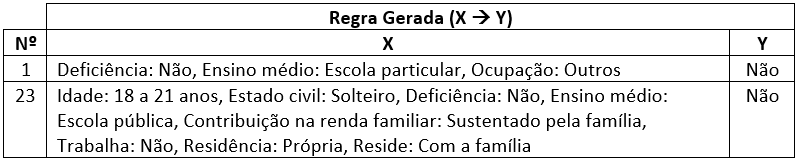
\includegraphics[scale=0.75]{Figuras/Suporte_15_Nao_atributos_22.png}
	\end{center}
\end{table}


\subsection{Observações nas Taxas de Confiança e Lift Para os Resultados Obtidos}

\par
\textcolor{red}{Nos resultado obtidos com o algoritmo de associação, para todos os casos que foram gerados as regras, a porcentagem de confiança de todas essas regras eram de 100\%, o motivo de todas elas possuírem essa taxa, foi pelo fato de que a base teve que ser dividida em duas partes (candidatos aprovados e não aprovados), para poder retirar a tendência  do algoritmo de gerar regras somente para os candidatos que não foram aprovados, que no caso, eram os que possuíam mais registros. Como o algoritmo foi aplicado em uma base onde a variável Aprovado possuía somente uma classe (Sim ou Nao), as regras geradas associadas para essa variável obtiveram resultados com 100\% de confiança, ou seja, a frequência na qual os atributos aparecem em transações que contenham a classe da variável Aprovado é sempre de 100\%, a para as duas bases. }

\par
\textcolor{red}{Comparando com trabalho de \citeonline{LeandroSilva2014} que serviu como base paras os testes deste trabalho, as regras que foram geradas para a sua base, possuíam taxas que variavam de 70\% a 100\% de confiança. O fator principal que influenciava essas porcentagens, foi porque, a variável principal deles a Nota da prova, continha 4 classes que possuíam quantidades de registros que não variavam muito entre elas, não possuíam uma classe que era mais predominante, ao contrario deste trabalho, que uma das classe possuía 10 vezes mais a quantidade de registro do que a outra classe. Para o caso do parâmetro Lift, que é uma métrica que classifica as melhores regras, o algoritmo classificou para todas as regras geradas, associada a variável Aprovado, o valor 1 de importância, ou seja, todas as regras obtidas possuem o mesmo grau de importância.}

\par
\textcolor{red}{Lembrando que outras regras foram geradas para os mesmos casos testados, onde elas possuíam confiança de 80\% a 90\% e lift abaixo e acima do valor 1, contudo, eles não foram mencionados neste trabalho, pelo fato de não serem associados a variável que é importante para esta pesquisa, no caso, a variável Aprovado.}

% ----------------------------------------------------------



% ----------------------------------------------------------
% Resultados -- Pode vir junto com discussão
% ----------------------------------------------------------
%\chapter{RESULTADOS EXPERIMENTAIS}
%\label{chapter:Resultados}

\par
\textcolor{red}{Nesta seção serão apresentados os resultados obtidos após as avaliações do modelo, que foi feito com os algoritmos de classificação e associação. Será demonstrado quais variáveis foram classificadas com maior relevância, as ramificações geradas com maior quantidade de registros que percorrem elas, além das regras obtidas para base através do algoritmo de associação.}

\section{Classificação}

\par
\textcolor{red}{Os resultados obtidos com o algoritmo de classificação apresentam um valor mediano de acurácia para o modelo utilizado. A técnica de classificação que foi utilizada, classificou corretamente em torno de 53\% das instâncias que pertence ao conjunto de teste, em relação à classe do resultado que foi obtido. Com base do modelo de árvore de decisão deduzido pelo algoritmo J48, foi possível analisar o grau de interação e a relação das variáveis de acordo com o caminho de interações percorrido pelas respostas do questionário feitas pelos candidatos.}

\par
\textcolor{red}{A árvore obtida apresentou como variável independente principal para a classificação o atributo Deficiencia, que se divide em 5 valores: Nao, Sim visual, Sim outro tipo, Sim fisica e Sim auditiva. As próximas variáveis com maior relevância mudavam de acordo com o valor que era obtido, sendo que, quando a resposta do candidato era de que ele não possuía alguma deficiência ou que ele possuía uma deficiência visual, a variável com maior importância para onde os valores eram direcionados era se ele frequentava ou frequenta cursinho particular, enquanto, para aqueles que possuíam deficiência física ou auditiva eram direcionados para a variável Cor (cor de pele), como apresentada na Figura 39.}

\par
\begin{figure}[!htp]
	\begin{center}
    \caption{\label{fig:waveform_fig} Representação das principais variáveis da árvore de decisão.}
	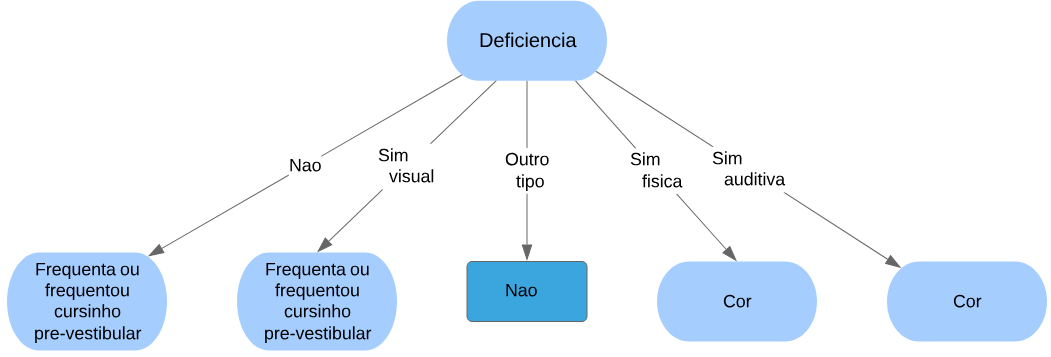
\includegraphics[scale=0.57]{Figuras/Arvore_gerada_grau2.png}
	\end{center}
    \legend{Fonte: Próprio autor.}
\end{figure}


\par
\textcolor{red}{É possível observar na Figura 37, que para os candidatos que responderam que possuíam outro tipo de deficiência, o valor da resposta era direcionado para um nó folha da classe Nao pertencente a variável dependente Aprovado, isto é, os candidatos que possuíam outro tipo de deficiência que não foram mencionados como opção de resposta da questão, não foram capazes de passar no vestibular (um total de 9 candidatos). A partir do terceiro nível de profundidade, para os candidatos que não possuíam nenhum tipo de deficiência a ramificação da árvore se expandia (tracejado pela linha vermelha), enquanto, diferentemente para os candidatos que possuíam algum tipo de deficiência, eles eram direcionados para os nós folhas da variável Aprovado (tracejado pela linha verde), como apresentado na Figura 40.}

\par
\begin{figure}[!htp]
	\begin{center}
    \caption{\label{fig:waveform_fig} Árvore completa.}
	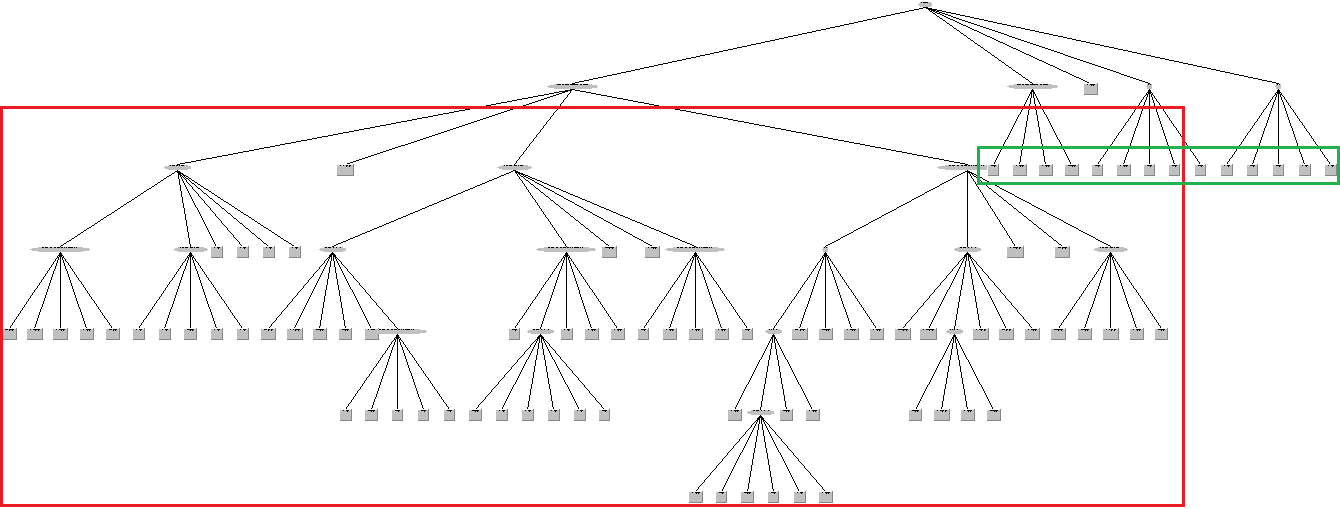
\includegraphics[scale=0.45]{Figuras/Arvore_completa.png}
	\end{center}
    \legend{Fonte: Próprio autor.}
\end{figure}


\subsection{Resultados Obtidos Para os Candidatos que não Possuiam Nenhum Tipo de Deficiência}


\par
\textcolor{red}{Avaliando a árvore que foi gerada, através da maior quantidade de registros que se encaixam pelo caminho percorrido das ramificações até as folhas, foi obtido os seguintes resultados, começando pela ramificação maior que era a dos candidatos que não possuiam nenhum tipo de deficiencia, a variavel com maior relevancia que foi classificada após o variavel independente principal era se o candidato frequentava um cursinho pré-vestibular. Foi classificado que todos aqueles que frequentaram por mais de um ano algum cursinho, não foram aprovados no vestibular.}

\par
\textcolor{red}{Para aqueles que frequentaram o cursinho por um ano, o atributo correspondente seguinte era a quantidade de pessoas que moravam com ele, sendo que, a maior taxa de candidatos aprovados para essa variavel era quando possuia 3 pessoas morando com ele e para reprovados era quando possuia de 4 a 5 pessoas. Já para os candidatos que ficavam por um semestre fazendo o cursinho, a variavel correspondente seguinte era o meio de transporte que ele utilizava, a maior taxa de aprovados era pra aqueles que usavam o transporte coletivo e para os reprovados eram os outros tipos de transportes não eram mencionados como opção de resposta.}

\par
\textcolor{red}{Para aqueles que não frequentavam algum cursinho pré-vestibular, a variável classificada com maior relevância, seguinte, era a quantidade de pessoas que moravam com o candidato, e dependendo dos valores que eram respondidos para essa variável, os atributos em sequência variavam entre cor de pele, ocupação do pai e meio de transporte utilizado. Foi notado que as maiores taxas de aprovados eram para os candidatos pardos, que moravam de 3 a 5 pessoas e que o pai era servidor público, já para aqueles que não foram aprovados, as maiores taxas eram quando o candidato possuía de quatro ou mais pessoas morando com ele, o pai possuía outro tipo de ocupação e o meio de transporte utilizado era o coletivo.}


\subsection{Resultados Obtidos Para os Candidatos que Possuem Algum Tipo de Deficiência}


\par
\textcolor{red}{Diferente dos valores classificados para os candidatos que não possuíam algum tipo de deficiência, para aqueles que possuíam, o nível de profundidade que a ramificação delas alcançou não foi tão grande quanto a outra. Os resultados obtidos foram, primeiro, para os candidatos que eram deficientes visuais, a taxa de maior aprovação na prova era para aqueles que não frequentaram cursinho pré-vestibular, enquanto para aqueles que frequentaram cursinho por mais de um ano a taxa de reprovação era maior.}

\par
\textcolor{red}{Foi possível observar que tanto para os candidatos com deficiência física quanto para auditiva, a variável que mais influenciava para que eles fossem aprovados ou não era cor de pele. Sendo que para os candidatos com deficiência física, aqueles que eram brancos a chance de ser aprovado era maior, diferente para aqueles que eram pardos tendo sua taxa de reprovação muito alta comparada a outros tons de pele.}

\par
\textcolor{red}{Para os candidatos que possuíam deficiência auditiva, aqueles que tinham um tom de pele pardo obtiveram as maiores taxas de aprovação, ao contrário daqueles que possuíam uma cor de pele branca, a taxa de reprovação era alta. Como já foi mencionado anteriormente na parte de avaliação do trabalho, os candidatos que possuíam qualquer outro tipo de deficiência, foram classificados, que nenhum deles tiveram êxito de serem aprovados no vestibular.}


\section{Associação}

\textcolor{red}{Através dos resultados obtidos com o algoritmo de associação, observou que a medida que o suporte mínimo decrescia, a quantidade de regras que eram geradas aumentava. Os resultados das regras geradas foram divididos em duas partes, para os candidatos aprovados e para os candidatos não aprovados.}

%\textcolor{red}{787 registros aprovados, 7784 registros não aprovados, 8571.}


\subsection{Regras Geradas Para os Candidatos Aprovados}

\par
\textcolor{red}{Analisando as regras geradas em cada teste, na Tabela 5 que apresenta a tabela das regras gerada utilizando 22 atributos com 50\% de suporte, são interpretados da seguinte maneira. Para regra com menor transição de itens, diz que se o candidato possui outro tipo de trabalho não mencionado e a sua residência é própria então ele terá chance de ser aprovado com 100\% de confiança. Já para a maior regra gerada, diz que se o candidato não possui alguma deficiência, seu ensino médio é todo em escola pública e possui outro tipo de trabalho não mencionado, então a chance de ele passar é de 100\% de confiança. Para ambas as regras, acontece com 5\% dos candidatos (394 instancias).}


\par
\begin{table}[!htp]
	\begin{center}
    \caption{\label{fig:waveform_fig} Suporte Mínimo 50\% e Confiança Mínima 70\%.}
	\includegraphics[scale=0.75]{Figuras/Suporte_50_atributos_22.png}
	\end{center}
\end{table}

\par
\textcolor{red}{Para os outros testes com 4 e 9 atributos, com a taxa de 50\% de suporte, nenhuma regra foi gerada para elas. Assim como os resultados do teste de 50\% de suporte, para os testes de 30\% das transições feitas com a quantidade de 4 e 9 atributos, nenhuma regra foi gerada também, já para a base com 22 atributos, foram geradas pelo menos 11 regras no geral, associadas com a variável Aprovados. Sendo que a primeira regra gerada possui 5 itens em sua transição e a última regra gerada chega a possuir 7 itens em sua transição. As regras foram geradas para 236 instancias (3\% dos candidatos), como apresentado na Tabela 6, onde é demonstrado a primeira e a ultima regra gerada.}

\par
\begin{table}[!htp]
	\begin{center}
    \caption{\label{fig:waveform_fig} Suporte Mínimo 30\% e Confiança Mínima 70\%.}
	\includegraphics[scale=0.75]{Figuras/Suporte_30_atributos_22.png}
	\end{center}
\end{table}


\par
\textcolor{red}{Avaliando os testes com 25\% de suporte mínimo, foram geradas regras para as bases com 9 e 22 atributos e para a base com 4 atributos nenhuma regra foi obtida. Analisando a única regra que foi gerada para a base com 9 atributos, diz que 2\% dos candidatos que eram aprovados (197 instancias), eles não trabalhavam, não possuíam algum tipo de deficiência e o meio de transporte utilizado era o coletivo, representado na Tabela 7. Já para a primeira regra gerada para a base com 22 atributos, 2\% dos candidatos que foram aprovados (197 instancias) eram solteiros, sustentados pela família e utilizava o transporte coletivo, como representado na Tabela 8.}

\par
\begin{table}[!htp]
	\begin{center}
    \caption{\label{fig:waveform_fig} Suporte Mínimo 25\% e Confiança Mínima 70\% para a base com 9 atributos.}
	\includegraphics[scale=0.75]{Figuras/Suporte_25_atributos_9.png}
	\end{center}
\end{table}

\par
\begin{table}[!htp]
	\begin{center}
    \caption{\label{fig:waveform_fig} Suporte Mínimo 25\% e Confiança Mínima 70\% para a base com 22 atributos.}
	\includegraphics[scale=0.75]{Figuras/Suporte_25_atributos_22.png}
	\end{center}
\end{table}

\par
\textcolor{red}{Com o suporte mínimo de 15\%, as bases de dados com 4 e 9 atributos obtiveram somente uma regra gerada, enquanto, para a base de dados com 22 atributos, foi obtido 67 regras geradas, sendo que é considerada a maior quantidade de regras que já foi gerada para todos os suportes mínimos testados. Começando com a regra gerada para a base com 4 atributos, como demonstrado na Tabela 9, indica que os candidatos que tem uma mãe com ensino médio completo e possui de 4 a 5 pessoas morando com eles, influenciam para que eles sejam aprovados.}

\par
\begin{table}[!htp]
	\begin{center}
    \caption{\label{fig:waveform_fig} Suporte Mínimo 15\% e Confiança Mínima 70\% para a base com 4 atributos.}
	\includegraphics[scale=0.75]{Figuras/Suporte_15_atributos_4.png}
	\end{center}
\end{table}

\par
\textcolor{red}{Já para a base com 9 atributos, a regra gerada indica que os candidatos que possuem um pai que é servidor público, mora com a família e possui de 4 a 5 pessoas morando com eles, são aprovados no vestibular, como apresentado na Tabela 10.}

\par
\begin{table}[!htp]
	\begin{center}
    \caption{\label{fig:waveform_fig} Suporte Mínimo 15\% e Confiança Mínima 70\% para a base com 9 atributos.}
	\includegraphics[scale=0.75]{Figuras/Suporte_15_atributos_9.png}
	\end{center}
\end{table}

\par
\textcolor{red}{Para a base de dados com 22 atributos com um suporte mínimo de 15\%, conforme é demonstrado da Tabela 11, na primeira regra gerada, a idade de 18 a 21 anos e a mãe como principal responsável, influenciavam para que o candidato fosse aprovado, enquanto para a última regra gerada, os candidatos que eram pardos, que não frequentavam cursinho pré-vestibular, nunca trabalharam e moravam com a família, eles eram aprovados. As regras geradas paras as bases com 4, 9 e 22 atributos, com um suporte de 15\%, influenciavam 1,4\% dos candidatos (118 instancias).}

\par
\begin{table}[!htp]
	\begin{center}
    \caption{\label{fig:waveform_fig} Suporte Mínimo 15\% e Confiança Mínima 70\% para a base com 22 atributos.}
	\includegraphics[scale=0.75]{Figuras/Suporte_15_atributos_22.png}
	\end{center}
\end{table}



\subsection{Regras Geradas Para os Candidatos que não Foram Aprovados}


\par
\textcolor{red}{Para os testes com a base de dados dos candidatos que não foram aprovados, dos 4 suportes mínimos utilizados, apenas 3 geraram regras para as bases de dados, que foram os suportes de 30\%, 25\% e 15\%, sendo que para os suportes testados, geraram regras somente para a base com 22 atributos. Começando com o suporte mínimo de 30\%, como podemos ver na Tabela 12, foi gerado apenas uma regra associada a variável de Aprovados, indicando que que 27\% dos candidatos (2.335 instancias) que não foram aprovados eles eram solteiros, com o tom de pele pardo, não trabalhavam e possuíam residência própria.}


\par
\begin{table}[!htp]
	\begin{center}
    \caption{\label{fig:waveform_fig} Suporte Mínimo 30\% e Confiança Mínima 70\% para a base com 22 atributos.}
	\includegraphics[scale=0.75]{Figuras/Suporte_30_Nao_atributos_22.png}
	\end{center}
\end{table}

\par
\textcolor{red}{Semelhante ao anterior, o suporte mínimo de 25\% gerou uma única regra, somente para a base de 22 atributos, como demonstrado na Tabela 13, a regra gerada indica que 22\% dos candidatos que não foram aprovados (1.946 instancias), eram solteiros, possuem uma renda mensal familiar de 2 a 4 salários mínimos, a residência deles é própria e moram com a família.}

\par
\begin{table}[!htp]
	\begin{center}
    \caption{\label{fig:waveform_fig} Suporte Mínimo 25\% e Confiança Mínima 70\% para a base com 22 atributos.}
	\includegraphics[scale=0.75]{Figuras/Suporte_25_Nao_atributos_22.png}
	\end{center}
\end{table}

\par
\textcolor{red}{Com um suporte mínimo de 15\%, foi obtido regras apenas para a base de dados com 22 atributos, tendo um total de 23 regras geradas. Para a primeira regra, os candidatos que não era deficiente, o ensino médio foi em escola particular e possuía outro tipo de trabalho que não foi mencionado nas opções dadas, eles não eram aprovados. Já para a última regra, para os candidatos com a idade entre 18 a 21 anos, solteiro, não possuía algum tipo de deficiência, o ensino médio foi em escola pública, era sustentado pela família, não trabalhava, possuía uma residência própria e morava com a família, todos esses fatores influenciavam para que eles não fossem aprovados, que era no total de 14\% dos candidatos (1.168 instancias), conforme o que é demonstrado na Tabela 14.}

\par
\begin{table}[!htp]
	\begin{center}
    \caption{\label{fig:waveform_fig} Suporte Mínimo 15\% e Confiança Mínima 70\% para a base com 22 atributos.}
	\includegraphics[scale=0.75]{Figuras/Suporte_15_Nao_atributos_22.png}
	\end{center}
\end{table}


\subsection{Observações nas Taxas de Confiança e Lift Para os Resultados Obtidos}

\par
\textcolor{red}{Nos resultado obtidos com o algoritmo de associação, para todos os casos que foram gerados as regras, a porcentagem de confiança de todas essas regras eram de 100\%, o motivo de todas elas possuírem essa taxa, foi pelo fato de que a base teve que ser dividida em duas partes (candidatos aprovados e não aprovados), para poder retirar a tendência  do algoritmo de gerar regras somente para os candidatos que não foram aprovados, que no caso, eram os que possuíam mais registros. Como o algoritmo foi aplicado em uma base onde a variável Aprovado possuía somente uma classe (Sim ou Nao), as regras geradas associadas para essa variável obtiveram resultados com 100\% de confiança, ou seja, a frequência na qual os atributos aparecem em transações que contenham a classe da variável Aprovado é sempre de 100\%, a para as duas bases. }

\par
\textcolor{red}{Comparando com trabalho de \citeonline{LeandroSilva2014} que serviu como base paras os testes deste trabalho, as regras que foram geradas para a sua base, possuíam taxas que variavam de 70\% a 100\% de confiança. O fator principal que influenciava essas porcentagens, foi porque, a variável principal deles a Nota da prova, continha 4 classes que possuíam quantidades de registros que não variavam muito entre elas, não possuíam uma classe que era mais predominante, ao contrario deste trabalho, que uma das classe possuía 10 vezes mais a quantidade de registro do que a outra classe. Para o caso do parâmetro Lift, que é uma métrica que classifica as melhores regras, o algoritmo classificou para todas as regras geradas, associada a variável Aprovado, o valor 1 de importância, ou seja, todas as regras obtidas possuem o mesmo grau de importância.}

\par
\textcolor{red}{Lembrando que outras regras foram geradas para os mesmos casos testados, onde elas possuíam confiança de 80\% a 90\% e lift abaixo e acima do valor 1, contudo, eles não foram mencionados neste trabalho, pelo fato de não serem associados a variável que é importante para esta pesquisa, no caso, a variável Aprovado.}
%\chapter{DISCUSSÃO}

% ----------------------------------------------------------
% Conclusão
% ----------------------------------------------------------
\chapter{Conclusão}
\label{chapter:consideracoes}

\subsection{Considerações Finais}

\par 
A mineração de dados se tornou uma ferramenta de suporte com papel essencial no gerenciamento da informação dentro das organizações. O manuseamento dos dados e a análise das informações que eram feitas de maneira convencional, se tornou impossível devido a imensa quantidade de dados que é coletado e armazenado em sua base diariamente. Encontrar padrões escondidos e relacionamentos em arquivos que possuem um grande volume de informações de forma manual, deixou de ser uma escolha. As técnicas de mineração passaram a ser utilizadas e começaram a estar presentes no nosso cotidiano.

\par
Com uma grande quantidade de dados que estão sendo armazenados pelas universidades e com recente surgimento de várias tecnologias e técnicas de extração de dados, uma boa parte dessas instituições estão tentando de alguma forma utilizar esses dados que são extraídos  na intenção de compreende-los e utiliza-los para benefício próprio. Como podemos observar nos trabalhos apresentado neste TCC, que através dos dados armazenado de candidatos que vão prestar o vestibular, foi gerado um perfil dos mesmos na intenção de descobrir os motivos que influenciam os seus desempenhos em sua aprovação.

\par
Desta forma, assim como os trabalhos apresentados, que tinham como objetivo de obter os perfis dos candidatos para identificar os fatores que influenciavam na sua aprovação, este trabalho, seguiu com o mesmo intuito tendo como base o software, os algoritmos e os métodos utilizados pelos mesmos. Os resultados obtidos através desses métodos utilizados, se mostraram bastante interessante em relação com a base de dados testada, apresentando perfis com algumas características semelhantes aos trabalhos mencionados. Entretanto, os atributos presentes na base dados em comparação aos trabalhos que foram usados como base, possuem um grau de relevância diferente, assim, como a taxa de precisão da performance dos algoritmos.

\par
O software WEKA durante o uso, demonstrou ser bastante robusto em termos de recursos em relação ao modelo que foi utilizado, o KDD. Sendo que ele apresentou várias utilidades em cada etapa do processo do modelo, desde a etapa do pré-processamento com a modelagem da base de dados até a etapa de pós-processamento, com apresentação dos resultados que foram obtidos através das técnicas e algoritmos implementados a essa API (como gráficos, tabelas, etc). As partes de configuração dos parâmetros dos algoritmos apresentado pelo software, se mostraram bastante intuitivos, facilitando com a manuseamento na parte do processo de mineração dos dados.

\par
Alguns problemas foram encontrados durante o processo de mineração, como o caso de um dos algoritmos utilizados que não conseguiu classificar os registros da base de dados.  Isso aconteceu, pelo fato do atributo principal que indicava quais candidatos foram aprovados, possuírem classes com o seus registros bastante desbalanceados. O problema teve que ser resolvido com o balanceamento dos valores das classes deste atributo, entretanto, teve como consequência uma diminuição da quantidade de registros da base de dados, fazendo com que o algoritmo perdesse um pouco da sua performasse.

\par
Dentre os dois algoritmos testados, o Apriori foi o que demonstrou maior desempenho com a base de dados utilizada, onde ele gerou regras bastante precisas que possuíam confiança acima da taxa que foi determinada de 70\%, chegando a 100\% de confiança. Enquanto o algoritmo J48 obteve uma taxa abaixo do que era desejado, com 53\% de precisão. Para as regras mais confiáveis, os atributos como: o tipo de deficiência do candidato, o estado civil que ele possui, a escola que passou o ensino médio e se ele trabalhava, eram fatores que influenciavam no resultado do desempenho deles na prova, no caso, se eles eram aprovados ou não.  

\par
De acordo com a análise e os parâmetros utilizados neste trabalho, através das regras obtidos pelos algoritmos de classificação e associação, conseguiu ser extraídos informações interessantes através dos perfis gerados pelas regras, tendo como uma taxa de precisão até que boa, em comparação à média entre os dois algoritmos. Dentre essas informações obtidas, analisando os atributos que formavam as regras, foi observado que o atributo que indicava o tipo de deficiência do candidato, teve como maior relevância para as regras obtidas nos dois algoritmos, sendo que em ambos os modelos, foi o atributo que apareceu com mais frequência. Analisando esse atributo mais afundo em relação aos candidatos que foram aprovados, foi observado que uma quantidade bem pequena desses candidatos apareciam nessa classificação, o que demonstra que esse fator pode indicar a falta de acessibilidade no sistema de educação que possuímos hoje.


%\par
%Em resumo, podemos perceber que a mineração de dados vem  cada vez mais sendo utilizada dentro da área educacional como em universidades, pois, com a imensa quantidade de dados que é armazenado, onde muitas vezes é repleta de informações importantes escondidas, se necessita dessas técnicas de mineração para se extrair esses dados com a intenção de usa-las, podendo assim relacionar informações contidas para predeterminar possíveis ações futuras na sua gestão com tutores, alunos e entre outros. Não resta dúvida de que a mineração de dados na área educacional está sendo extremamente promissora e que, apesar dos resultados já alcançados, ainda ela tem muito para o que oferecer.

\subsection{Trabalhos Futuros}

\par
Neste trabalho, foram tratados apenas o desempenho dos candidatos em relação a sua aprovação no vestibular, a partir dos dados socioeconômicos obtidos, contudo, pode ser feita a analise de outros tipos de desempenhos, como é o caso das escolas. Através do histórico escolar de ensino médio dos candidatos que é armazenado pela universidade, pode-se pegar as notas que se encontram nesse histórico, e fazer uma média com elas, para poder verificar o desempenho das escolas em relação ao resultado do desempenho dos alunos no vestibular. 

\par
Outro tipo de analise que pode ser feita, é a chance do candidato de concluir o curso em que ele foi aprovado. Onde, a partir dos perfis que foram gerados, será analisado a probabilidade do candidato em concluir o curso que ele escolheu, através da utilização de um algoritmo treinado com base nos perfis dos acadêmicos que se formaram nos anos anteriores.

\par
Podemos sugerir também, uma análise temporal do desempenho dos candidatos, onde, pegaria a base de dados dos vestibulares anteriores em relação ao ano da base de dados em que está sendo utilizada e identificaria através da mineração, os fatores que mais ocorrem entre esses anos. Analisando assim, o progresso de influência de um determinado fator na aprovação dos candidatos, o período em que mais ocorreu e quais candidatos foram afetados por esses tipos de fatores.

%\newpage
% ----------------------------------------------------------
% Referências bibliográficas
% ----------------------------------------------------------
\bibliography{main}

%---------------------------------------------------------------------
% INDICE REMISSIVO
%---------------------------------------------------------------------
%\phantompart
%\printindex
%---------------------------------------------------------------------

\end{document}

